
% ════════════════════════════════════════════
% 模型的建立与求解（一级章节）写作规则 —— 模板内嵌，AI 先读本文件再写
% ════════════════════════════════════════════
% 【结构】本文件是一级标题「模型的建立与求解」的包装：\section{模型的建立与求解}，内部由下方「__SUBS__ 占位」注入
%   其「子块（二级标题）」的 \input 列表，子块来自 subs/ 下（如 5.1问题1的建立求解、5.2问题2的建立求解…）。
% 【生成】按题目小问数 N 选择 subs/ 下的子块并在组成里排序：N 问就 \input 5.1~5.N；N>4 新建，N<4 删除多余。
% 【每问骨架】每个 5.X.问题X的建立求解 用 \subsection{问题X的模型的建立和求解}，内部再 \input 四个三级子块，顺序固定为：
%   ① 具体分析（问题类型+方法+步骤+流程图）→ ② 模型准备（数据预处理+算法选择）→ ③ 模型建立（分题型建模）→ ④ 模型求解（结果表/图）。组合题型按题目主要类型选择，不必全部选。
% 【图片来源】论文用 求解/问题X/图片/xxx.png 引用；数据用 求解/问题X/结果/ 的 CSV。
% ════════════════════════════════════════════
\section{模型的建立与求解}

\subsection{问题一的模型的建立和求解}

\subsubsection{具体分析}

针对问题一，本问属于\textbf{综合评价与回归建模}类问题，需要完成三项递进任务：一是对 22 个质量指标进行预处理并建立综合评价模型，给出样本级、语料级与领域级质量评分 $Q$；二是定义并消解不同质量指标之间的冲突；三是建立 17 域配比 $\bm p$ 与交叉熵损失之间的定量关系并验证。本问综合采用指标方向统一、极差归一化与熵权法进行质量评价，采用成对标准化得分差与 Kendall 协同系数进行冲突检验与消解，采用岭正则线性混合回归（Ridge Mixture Regression）刻画配比—损失关系\cite{xie2023doremi}。

首先对质量信号数据进行清洗，将 22 个质量指标（含 8 个多维列表型指标）统一为“越高越好”的方向并压缩为标量，建立综合评价模型得到质量评分 $Q$；接着定义“冲突”为两指标标准化得分之差超过阈值的情形，用 Kendall 协同系数检验指标一致性并给出消解规则；然后利用训练配方表与损失表建立配比 $p_k$ 到各域损失 $L_d$ 的线性混合回归模型，并以岭正则处理成分数据的闭合效应与未测量域；最后在 1M、60M、1B 三套检验集上验证，并利用 10B、70B 外推表讨论跨尺度外推的稳健性。

\subsubsection{模型准备}

\textbf{1.数据预处理}

附件 A 的配方表（A4）以 17 个 The Pile 子领域的训练配比 $p_k$（分量非负且和为 1）为特征\cite{gao2020pile}，损失表（A5）以 13 个验证域的交叉熵损失为响应，二者通过 index 列一一对应。17 个训练域中 nih\_exporter、enron\_emails、europarl、philpapers 仅有配比列而无对应损失列，本文保留其配比分量但在系数解释时标注为“间接影响域”。质量信号数据（A1--A3）含 22 个质量指标，其方向并不统一，须先逐指标统一为“越高越好”。设第 $j$ 个指标的原始取值为 $x_j$，对正向指标直接做极差归一化，对负向指标先取补再归一化，对“长度型”指标（过长过短均不佳）转为中心接近度：
\begin{equation}
    x'_j = \begin{cases}
        \dfrac{x_j-\min x_j}{\max x_j-\min x_j}, & \text{正向指标}\\[6pt]
        \dfrac{\max x_j-x_j}{\max x_j-\min x_j}, & \text{负向指标}\\[6pt]
        \exp\!\left(-\dfrac{|\ln(1+x_j)-m_j|}{2.5\,\text{MAD}_j}\right), & \text{长度型指标}
    \end{cases}
\end{equation}
其中 $m_j$ 与 $\text{MAD}_j$ 为对数尺度的中位数与中位绝对偏差；$x'_j\in[0,1]$ 且统一为“越高越好”。22 个指标的方向判定与语义说明见表\ref{tab:p1_dir}，其中 8 个多维列表型指标（原始为有序类别 logits）先按 softmax 概率取归一化期望级别压缩为标量，再参与归一化。

\begin{longtable}{>{\raggedright\arraybackslash}p{0.30\textwidth}>{\centering\arraybackslash}p{0.12\textwidth}>{\raggedright\arraybackslash}p{0.20\textwidth}>{\centering\arraybackslash}p{0.10\textwidth}>{\centering\arraybackslash}p{0.12\textwidth}}
  \caption{22 个质量指标的方向判定与熵权}
  \label{tab:p1_dir} \\
  \toprule
  指标 & 类型 & 语义（方向依据） & 方向 & 熵权 $w_j$ \\
  \midrule
  \endfirsthead
  \caption{22 个质量指标的方向判定与熵权（续）} \\
  \toprule
  指标 & 类型 & 语义（方向依据） & 方向 & 熵权 $w_j$ \\
  \midrule
  \endhead
  \bottomrule
  \endfoot
  fineweb\_edu & 列表(1) & 教育价值 & 正向 & 0.0437 \\
  fluency\_en & 列表(2) & 英语流畅度（第 1 类=流畅，已核验） & 正向 & 0.0682 \\
  modernbert\_cleanliness & 列表(6) & 文本洁净度 & 正向 & 0.1434 \\
  modernbert\_readability & 列表(6) & 可读性 & 正向 & 0.0567 \\
  modernbert\_reasoning & 列表(6) & 推理性 & 正向 & \textbf{0.1517} \\
  modernbert\_professionalism & 列表(6) & 专业性 & 正向 & 0.0396 \\
  dsir\_books & 标量 & 书籍域重要性权重 & 正向 & 0.0081 \\
  dsir\_wiki & 标量 & 维基域重要性权重 & 正向 & 0.0081 \\
  dsir\_math & 标量 & 数学域重要性权重 & 正向 & 0.0086 \\
  qurater & 列表(4) & 教育质量评级（4 项取均值） & 正向 & 0.0492 \\
  ad\_en & 列表(2) & 广告含量（\textbf{第 1 类=“无广告”，正向}；依据：原文抽查） & 正向 & 0.0072 \\
  rps\_doc\_word\_count & 标量 & 文档词数 & 长度型 & 0.0516 \\
  rps\_doc\_num\_sentences & 标量 & 文档句数 & 长度型 & 0.0523 \\
  rps\_doc\_unigram\_entropy & 标量 & 一元词熵（多样性） & 正向 & 0.0347 \\
  rps\_doc\_frac\_unique\_words & 标量 & 唯一词占比 & 正向 & 0.0538 \\
  rps\_doc\_frac\_no\_alph\_words & 标量 & 非字母字符占比 & 负向 & 0.0287 \\
  rps\_doc\_frac\_chars\_top\_2gram & 标量 & 字符 2-gram 重复度 & 负向 & 0.0130 \\
  rps\_doc\_frac\_chars\_top\_3gram & 标量 & 字符 3-gram 重复度 & 负向 & 0.0119 \\
  rps\_lines\_uppercase\_letter\_fraction & 标量 & 大写字母行占比 & 负向 & 0.0316 \\
  rps\_lines\_ending\_with\_terminal\_punctution\_mark & 标量 & 终止标点结尾行占比 & 正向 & 0.0880 \\
  rps\_lines\_numerical\_chars\_fraction & 标量 & 含数字行占比 & 负向 & 0.0125 \\
  rps\_doc\_mean\_word\_length & 标量 & 平均词长 & 长度型 & 0.0373 \\
\end{longtable}

样本级质量评分由各指标加权求和得到，领域级质量 $Q_d$ 为该领域内样本评分的均值：
\begin{equation}
    Q_i = \sum_{j=1}^{22} w_j\, x'_{ij},\qquad Q_d=\frac{1}{n_d}\sum_{i\in\mathcal D_d}Q_i,\qquad \sum_j w_j=1
\end{equation}
其中权重 $w_j$ 由熵权法确定。由表\ref{tab:p1_dir}可见，权重最大的两项是 modernbert\_reasoning（$0.152$）与 modernbert\_cleanliness（$0.143$），即“推理性”与“洁净度”两个信号提供的信息量最多；需要说明的是，熵权法对取值分布的形态较敏感（极端左偏的指标会获得更大权重），因此本文在误差分析中对赋权方案作了敏感性检验（见第\ref{sec:check}节）。

质量信号存在少量字段级缺失，本文流式读取时逐字段审计，结果见表\ref{tab:p1_missing}，并按该指标中位数填充，不把缺失当作高质量或低质量。

\begin{longtable}{>{\raggedright\arraybackslash}p{0.44\textwidth}>{\centering\arraybackslash}p{0.16\textwidth}>{\raggedright\arraybackslash}p{0.36\textwidth}}
  \caption{质量信号的字段级缺失审计（A1--A3 全量 272{,}505 条）}
  \label{tab:p1_missing} \\
  \toprule
  指标 & 缺失记录数 & 形态 \\
  \midrule
  \endfirsthead
  \caption{质量信号的字段级缺失审计（续）} \\
  \toprule
  指标 & 缺失记录数 & 形态 \\
  \midrule
  \endhead
  \bottomrule
  \endfoot
  modernbert\_reasoning & 13 & 整行 6 维取值均为 NaN \\
  modernbert\_professionalism & 6 & 整行 6 维取值均为 NaN \\
  其余 20 个指标 & 0 & 无缺失 \\
\end{longtable}

\textbf{2.算法选择}

本问涉及质量评价（指标聚合）、冲突分析（一致性检验）与配比建模（回归）三类任务，需在候选算法中择优。质量聚合比较熵权法、主成分分析（PCA）第一主成分与等权平均；冲突分析以成对标准化得分差为主、Kendall 协同系数为辅；配比建模比较普通最小二乘、岭回归与随机森林。质量聚合的三种方案对比如表\ref{tab:algo1}所示。

\begin{longtable}{>{\centering\arraybackslash}p{0.20\textwidth}>{\centering\arraybackslash}p{0.16\textwidth}>{\centering\arraybackslash}p{0.20\textwidth}>{\raggedright\arraybackslash}p{0.36\textwidth}}
  \caption{问题一赋权方案对比（样本级相关性与域级排序一致性）}
  \label{tab:algo1} \\
  \toprule
  方案 & 得分均值 & 与熵权法相关性 & 域级 Spearman 排序一致性（对熵权法） \\
  \midrule
  \endfirsthead
  \caption{问题一赋权方案对比（续）} \\
  \toprule
  方案 & 得分均值 & 与熵权法相关性 & 域级 Spearman 排序一致性（对熵权法） \\
  \midrule
  \endhead
  \bottomrule
  \endfoot
  熵权法 & 0.495 & 1.000 & 1.000 \\
  等权平均 & 0.639 & 0.854 & 0.679 \\
  PCA 第一主成分 & 0.520 & 0.881 & 0.679 \\
\end{longtable}

如表\ref{tab:algo1}所示，熵权法能依据指标自身信息量客观赋权、避免主观打分；与等权方案相比，样本级得分相关系数为 $0.854$、域级排序一致性为 $0.679$，说明主体格局稳定但并非完全一致——改用等权后领域排序会发生变化，故本文在误差分析中把赋权方案列入灵敏度检验。PCA 方案虽降维去相关，但主成分含义难以解释，受篇幅限制不作备选。配比建模中 17 域配比满足单纯形约束（和为 1）而天然存在共线性，岭回归通过 $L_2$ 正则化能稳定估计且外推可解释，故采用岭正则线性混合回归。冲突分析方面，Kendall 协同系数刻画的是“指标作为评价者”的整体一致性，而问题要求的是“对同一文本给出显著不一致评价”的样本级冲突，二者互补，故同时报告。

\subsubsection{模型建立}

\textbf{步骤1：质量评价模型}

设 $m$ 条质量信号样本、22 个指标经方向统一与归一化后构成矩阵 $\bm X=(x'_{ij})$。第 $j$ 个指标的信息熵与熵权为：
\begin{equation}
    e_j = -\frac{1}{\ln m}\sum_{i=1}^{m} f_{ij}\ln f_{ij},\qquad f_{ij}=\frac{x'_{ij}+\varepsilon}{\sum_i (x'_{ij}+\varepsilon)},\qquad
    w_j = \frac{1-e_j}{\sum_{j=1}^{22}(1-e_j)}
\end{equation}
为与附件 B 的损失数据耦合，本问同时给出“结果导向”的领域质量代理指标：以各验证域在平均配方下的观测损失表征领域内在难度并映射为质量：
\begin{equation}
    Q_d^{(\text{loss})}=1-\frac{\bar L_d-\min_d \bar L_d}{\max_d \bar L_d-\min_d \bar L_d}
\end{equation}
其中 $\bar L_d$ 为领域 $d$ 的平均交叉熵损失。该代理指标仅在 13 个可测损失域上有定义，与 A1--A3 的 7 个质量域并非同一分类体系，二者的关联由 A16 映射表建立、并在模型求解中作一致性检验。

\textbf{步骤2：质量冲突消解模型}

当两个质量指标对同一文本给出显著不一致的评价时即产生冲突。以方向统一后的标准化得分为基础，定义第 $i$ 样本在指标 $j$ 与 $k$ 上的冲突指示：
\begin{equation}
    \delta_i(j,k) = \left| z_{ij} - z_{ik} \right|,\qquad z_{ij}=\frac{x'_{ij}-\mu_j}{\sigma_j},\qquad
    \mathbf 1\{\delta_i(j,k)>\tau\}
\end{equation}
取阈值 $\tau=1.5$；全样本冲突率为
\begin{equation}
    \rho_c = \frac{1}{m\binom{22}{2}}\sum_{i=1}^{m}\sum_{j<k}\mathbf 1\{\delta_i(j,k)>\tau\}
\end{equation}
为给出参照系，本文同时计算“指标独立”基准 $\rho_0=2\Phi(-\tau/\sqrt2)$：若 $\rho_c/\rho_0<1$，说明指标间存在正相关、并非互相矛盾。指标间整体一致性用 Kendall 协同系数检验（22 个指标为评价者、$m$ 条文本为评价对象）：
\begin{equation}
    W = \frac{12\sum_i (R_i-\bar R)^2}{22^2\,(m^3-m)},\qquad R_i=\sum_{j=1}^{22} r_{ij},\qquad
    \chi^2 = 22(m-1)W
\end{equation}
其中 $r_{ij}$ 为第 $i$ 样本在第 $j$ 指标上的秩。消解规则为：若某样本被判为冲突，则以其上“多数指标”的方向（即加权得分 $Q_i$ 相对该样本所在域中位数的偏离方向）作为该样本的最终质量裁决，并在报告中保留冲突标记以供下游剔除或降权。

\textbf{步骤3：领域配比建模（线性混合回归）}

设训练配方矩阵 $\bm P\in[0,1]^{n\times 17}$（行和为 1），损失矩阵 $\bm L\in\mathbb R^{n\times 13}$。建立各验证域损失对配比的线性混合模型：
\begin{equation}
    L_{d}(\bm p) = \sum_{k=1}^{17} a_{dk}\, p_k + b_d,\qquad d=1,\dots,13
    \qquad\Longleftrightarrow\qquad
    \hat{\bm L} = \bm P \bm A + \bm 1 \bm b^{\top}
\end{equation}
由于 $\bm P$ 各行和为 1，回归存在闭合不可辨识性，采用岭正则估计系数矩阵 $\bm A\in\mathbb R^{17\times 13}$ 与截距 $\bm b$：
\begin{equation}
    \min_{\bm A,\bm b}\ \left\|\bm L-\bm P\bm A-\bm 1\bm b^{\top}\right\|_F^2 + \lambda\left\|\bm A\right\|_F^2,
    \qquad
    \begin{bmatrix}\bm A\\ \bm b^{\top}\end{bmatrix}
    = \left(\tilde{\bm P}^{\top}\tilde{\bm P}+\lambda \bm D\right)^{-1}\tilde{\bm P}^{\top}\bm L
\end{equation}
其中 $\tilde{\bm P}=[\bm P,\ \bm 1]$，$\bm D=\mathrm{diag}(1,\dots,1,0)$（不惩罚截距），$\lambda=10^{-3}$。

\textbf{步骤4：质量信息的引入方式与检验}

问题一要求论证“是否以及如何引入质量评分 $Q$”。本文构造混合质量指数 $\bar Q(\bm p)=\sum_k p_k Q_k$（$Q_k$ 由 A16 映射得到：direct/near\_direct 域直接取用 A1--A3 域级质量，inferred 域取全局均值），并做增量回归检验：
\begin{equation}
    \hat{\bm L} = \bm P \bm A + \bm 1 \bm b^{\top} + \bm 1\, c^{\top}\bar Q(\bm p)
\end{equation}
若质量项带来的 $R^2$ 增量可忽略，则说明线性配比已吸收质量信息，此时不宜重复引入以免共线；质量评分转而作为独立资源交由问题二、三使用。

\textbf{步骤5：最优配比与稳健推荐}

在系数矩阵 $\bm A$ 基础上，固定未测量域配比于参考值，优化 13 个可测域的配比使加权平均损失最小：
\begin{equation}
    \min_{\bm p\in\Delta_{17}}\ \sum_{d\in\mathcal M} w_d\left(\sum_k a_{dk}p_k+b_d\right),
    \qquad \Delta_{17}=\left\{\bm p:\ p_k\ge0,\ \textstyle\sum_k p_k=1\right\}
\end{equation}
为给出可落地的稳健方案，进一步限制各域配比不超过参考配比的 2.5 倍，得到有界推荐配比。

\subsubsection{模型求解}

基于上述模型，利用附件 A 的质量信号（A1--A3）与配方/损失数据（A4--A15）进行求解，共处理全量质量记录 $272{,}505$ 条（A1 抽样集 $51{,}230$ 条、A2+A3 扩展集 $221{,}275$ 条）。

\textbf{1.质量评分与冲突分析}

质量域的领域级评分如图\ref{fig:p1_quality_full}所示，A1 抽样集与扩展集的对照结果如表\ref{tab:p1_qa}所示。

\begin{figure}[ht]
  \centering
  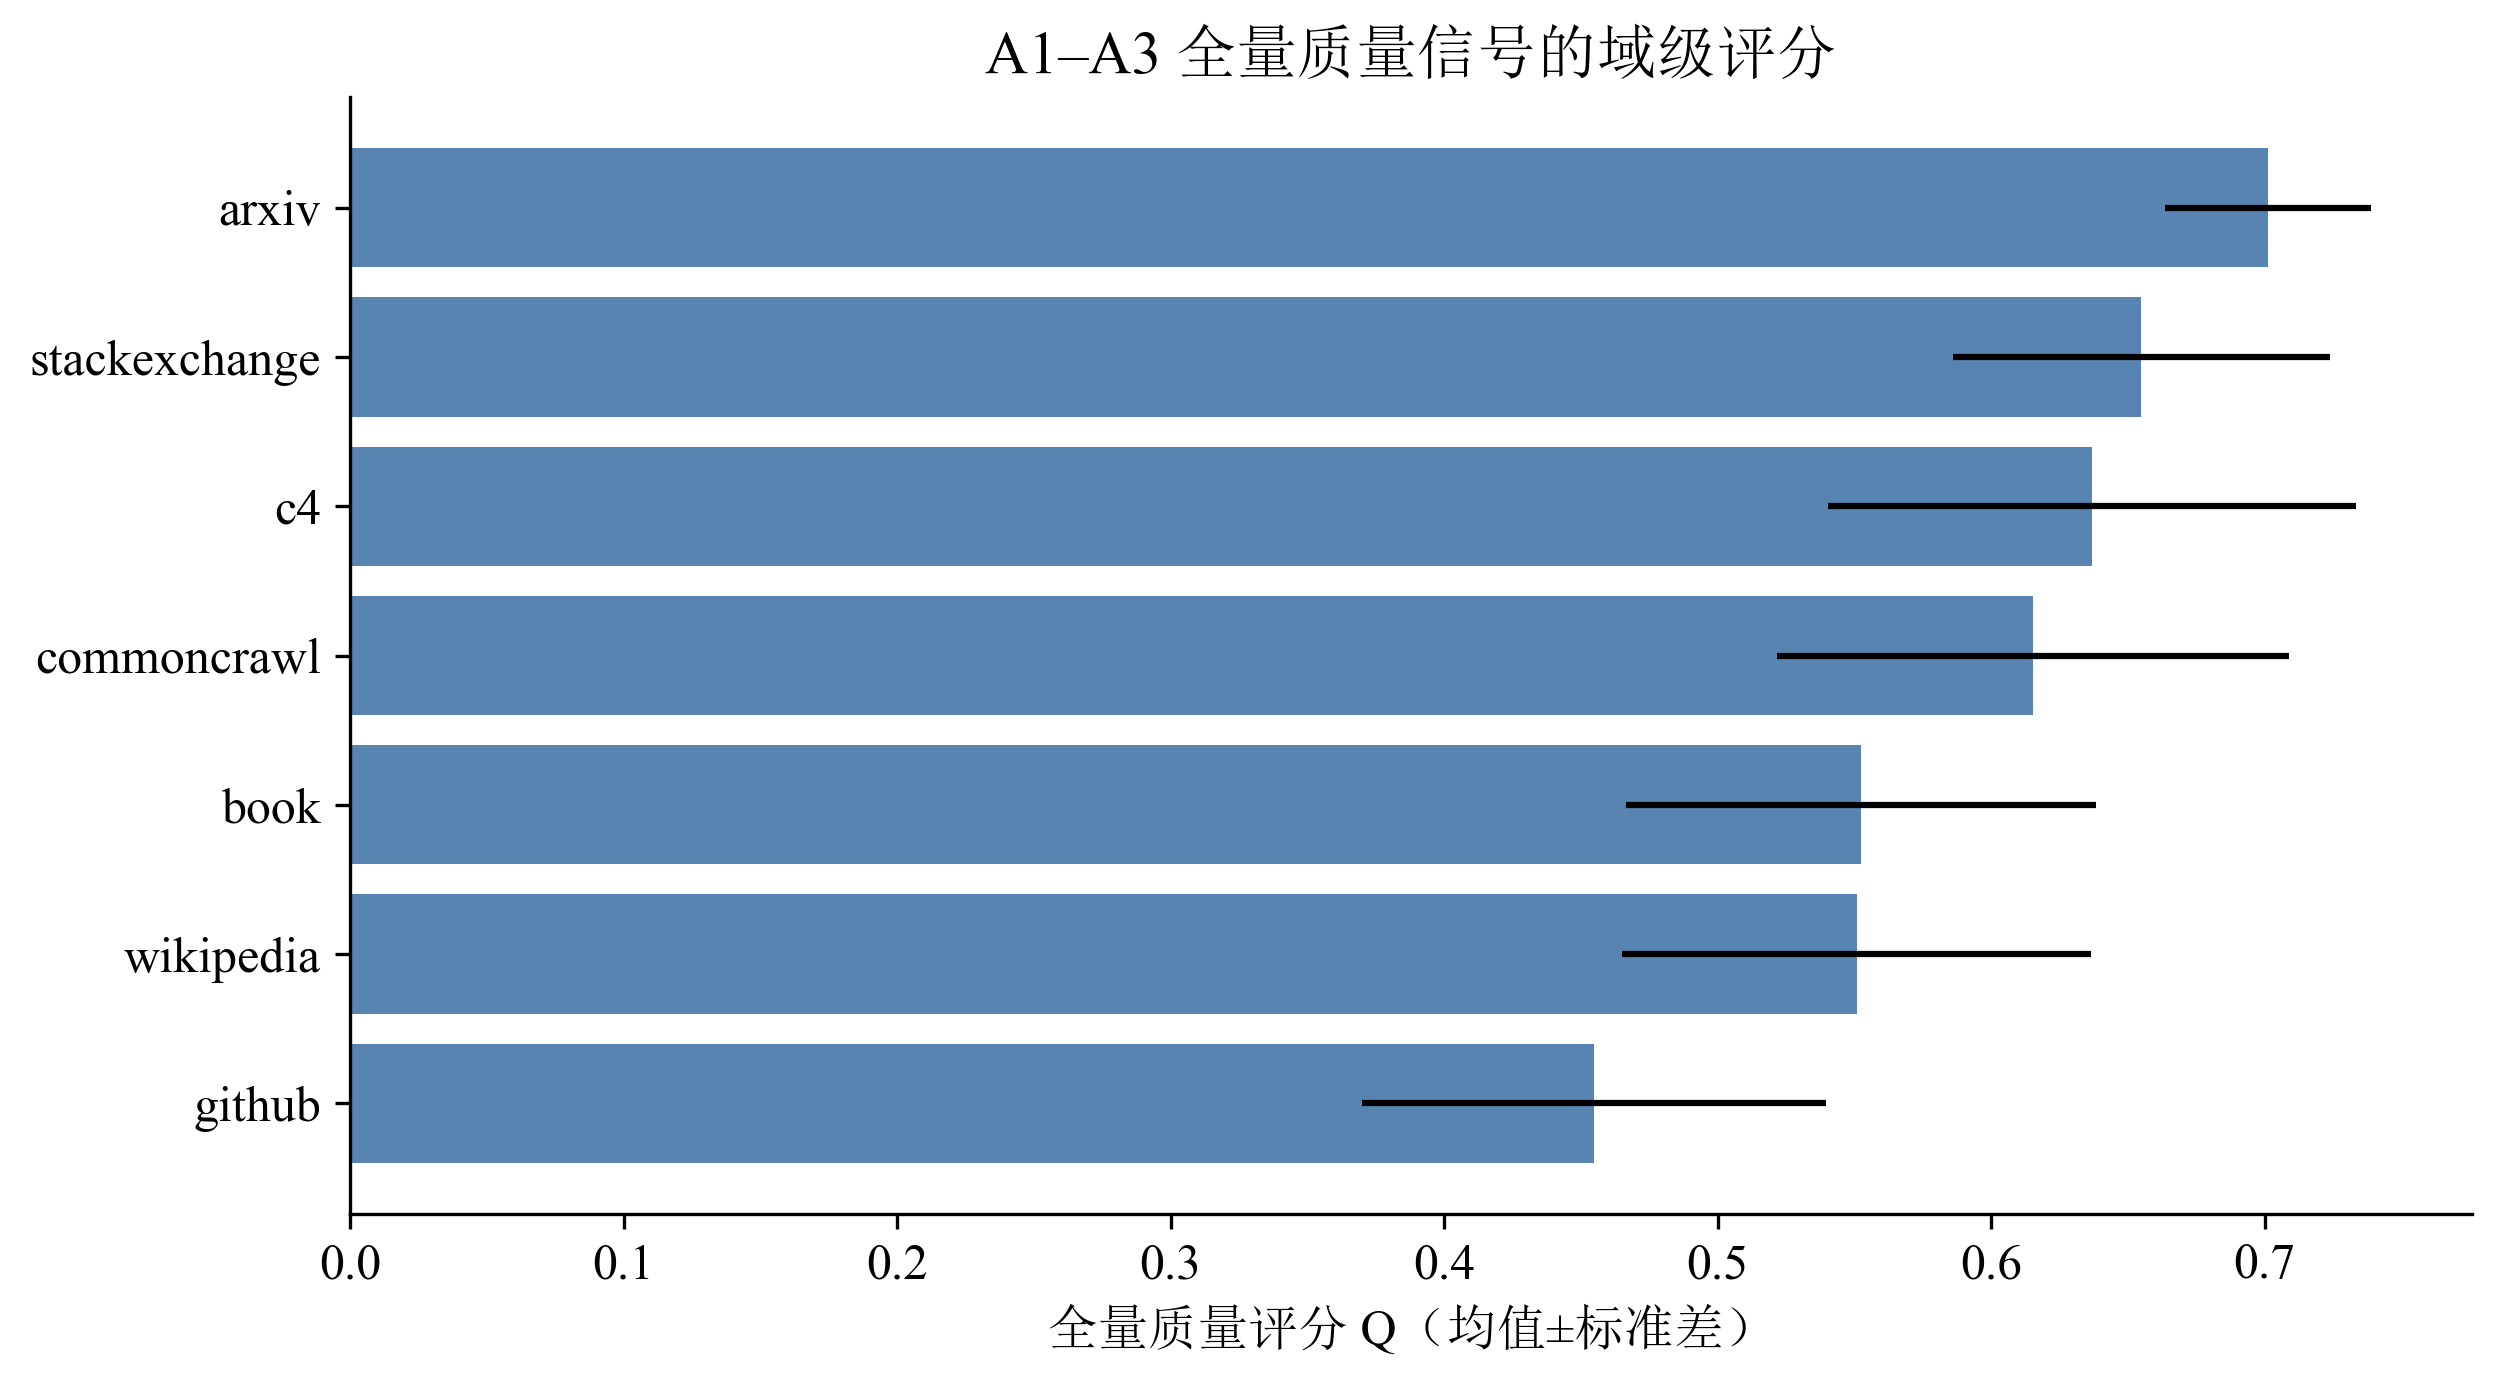
\includegraphics[width=0.62\textwidth]{求解/问题一/图片/图0_A1-A3全量质量评分.png}
  \caption{A1--A3 全量质量信号的领域级评分（均值±标准差）}
  \label{fig:p1_quality_full}
\end{figure}

\begin{longtable}{>{\centering\arraybackslash}p{0.20\textwidth}>{\centering\arraybackslash}p{0.16\textwidth}>{\centering\arraybackslash}p{0.16\textwidth}>{\centering\arraybackslash}p{0.16\textwidth}>{\raggedright\arraybackslash}p{0.24\textwidth}}
  \caption{抽样集 A1 与扩展集 A2/A3 的域级质量对照}
  \label{tab:p1_qa} \\
  \toprule
  质量域 & $Q$（A1） & $Q$（扩展集） & 差值 & 对应配方域 \\
  \midrule
  \endfirsthead
  \caption{抽样集 A1 与扩展集 A2/A3 的域级质量对照（续）} \\
  \toprule
  质量域 & $Q$（A1） & $Q$（扩展集） & 差值 & 对应配方域 \\
  \midrule
  \endhead
  \bottomrule
  \endfoot
  arxiv & 0.7031 & 0.7011 & $+0.0021$ & arxiv \\
  stackexchange & 0.6549 & — & — & stackexchange \\
  c4 & 0.6368 & — & — & （配方侧无同名列） \\
  commoncrawl & 0.6153 & — & — & pile\_cc \\
  book & 0.5524 & — & — & gutenberg\_pg\_19 \\
  wikipedia & 0.5509 & — & — & wikipedia\_en \\
  github & 0.4553 & 0.4547 & $+0.0006$ & github \\
\end{longtable}

由表\ref{tab:p1_qa}可知，在同时具有抽样与扩展质量信号的两个域上（arxiv、github），两种口径的域级质量差异不超过 $0.002$（arxiv $+0.0021$、github $+0.0006$），说明抽样集对扩展集具有代表性、评分口径可跨集合迁移。全体记录的领域质量排序为 arxiv（0.703）$>$ stackexchange（0.655）$>$ c4（0.637）$>$ commoncrawl（0.615）$>$ book（0.552）$\approx$ wikipedia（0.551）$>$ github（0.455）。需要指出，该排序是 22 个分类器信号的合成结果，其中若干信号（如 rps\_doc\_frac\_unique\_words、rps\_doc\_unigram\_entropy）与文档长度相关，因此“c4/commoncrawl 高于 book/wikipedia”反映的是信号体系的口径，而非对语料价值的终极判断——这一点在使用该评分时须注意。

冲突与一致性检验结果如表\ref{tab:p1_conf}所示，冲突最集中的指标对与熵权分布见图\ref{fig:p1_conf}。

\begin{longtable}{>{\centering\arraybackslash}p{0.18\textwidth}>{\centering\arraybackslash}p{0.13\textwidth}>{\centering\arraybackslash}p{0.13\textwidth}>{\centering\arraybackslash}p{0.13\textwidth}>{\centering\arraybackslash}p{0.14\textwidth}>{\raggedright\arraybackslash}p{0.20\textwidth}}
  \caption{质量冲突与一致性检验结果}
  \label{tab:p1_conf} \\
  \toprule
  数据集 & 样本数 & Kendall $W$ & 冲突率 $\rho_c$ & 独立基准 $\rho_0$ & $\rho_c/\rho_0$ \\
  \midrule
  \endfirsthead
  \caption{质量冲突与一致性检验结果（续）} \\
  \toprule
  数据集 & 样本数 & Kendall $W$ & 冲突率 $\rho_c$ & 独立基准 $\rho_0$ & $\rho_c/\rho_0$ \\
  \midrule
  \endhead
  \bottomrule
  \endfoot
  A1 抽样集 & 51{,}230 & 0.0783 & 0.2252 & 0.2888 & 0.780 \\
  A2+A3 扩展集 & 221{,}275 & 0.0628 & 0.2208 & 0.2888 & 0.764 \\
  全量 & 272{,}505 & 0.0687 & 0.2235 & 0.2888 & 0.774 \\
\end{longtable}

\begin{figure}[ht]
  \centering
  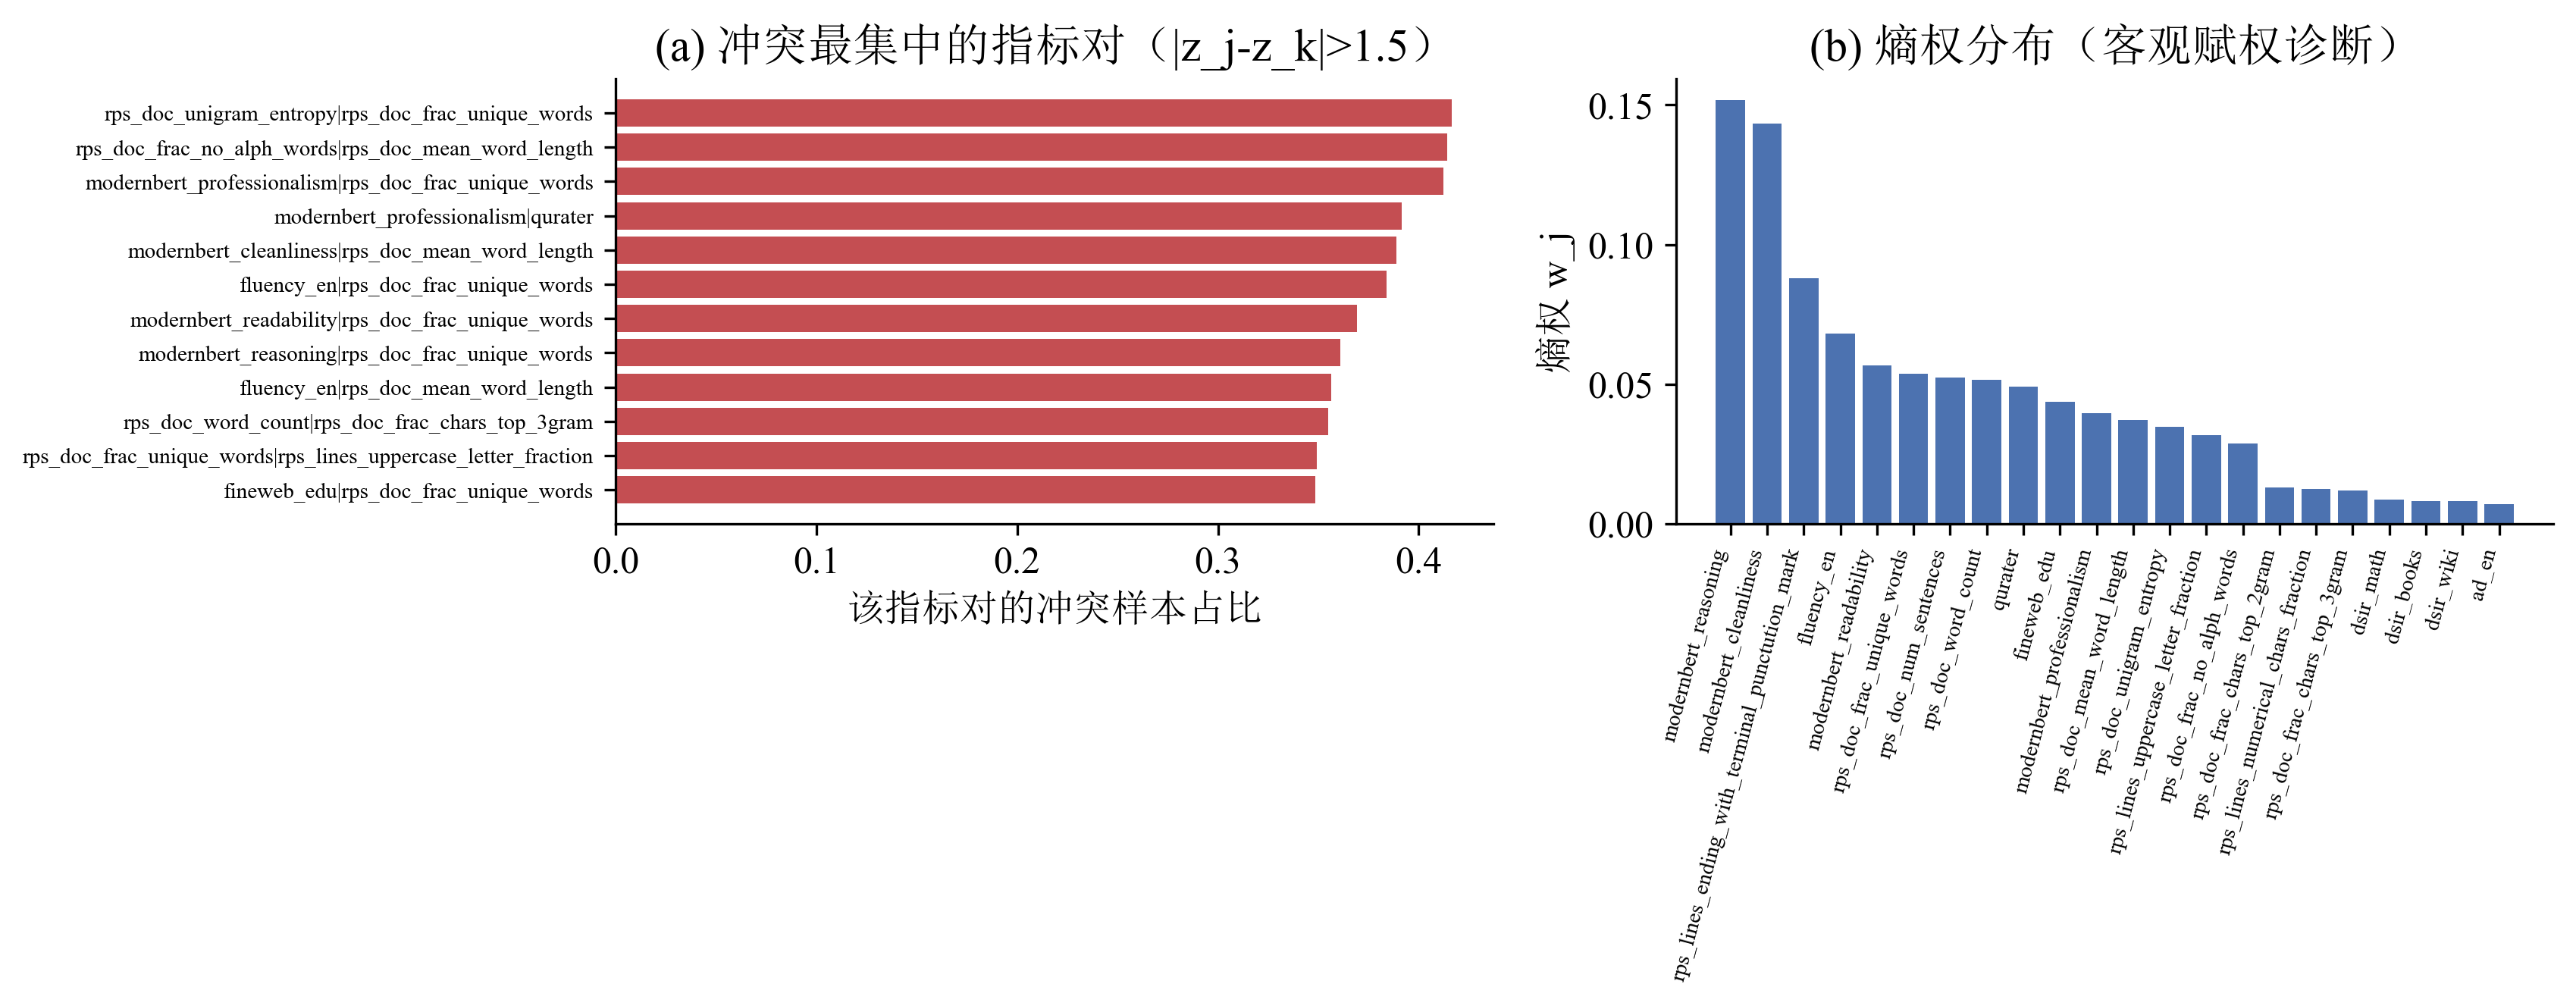
\includegraphics[width=0.92\textwidth]{求解/问题一/图片/图6_冲突与赋权诊断.png}
  \caption{冲突最集中的指标对（左）与熵权分布（右）}
  \label{fig:p1_conf}
\end{figure}

由表\ref{tab:p1_conf}可知：（1）三套数据的冲突率几乎一致（$0.221\sim0.225$），说明冲突结构在抽样集与扩展集上同样成立，A2/A3 的结论可外推至 A1 所代表的总体；（2）Kendall 协同系数为 $0.069$（$\chi^2$ 检验 $p<0.001$，样本量极大故显著性很高），属于“正相关但一致性较弱”的水平，与冲突率 $22.3\%$ 一致，说明“各质量指标完全一致、不存在冲突”的判断并不成立；（3）但冲突率低于指标完全独立时的基准 $28.9\%$（比值 $0.774$），说明指标间确为正相关，冲突主要发生在语义上本就不同的指标之间。冲突成因可归纳为三类：一是度量对象不同（如 rps\_doc\_unigram\_entropy 与 rps\_doc\_frac\_unique\_words 同测“多样性”但量纲不同），二是内容类型差异（如 modernbert\_professionalism 对学术文本与论坛文本的评价尺度不同），三是分布形态差异（如 ad\_en 为二分类概率、在长文档上两极化）。据此本文按“多数指标方向裁决 + 冲突标记保留”的规则消解：冲突样本仍参与领域均值，但以 $Q_i$ 相对域中位数的偏离方向标注其可信度，并在问题二、三中不单独使用冲突样本。

\textbf{2.配比—损失建模与验证}

配方结构与拟合、泛化表现分别如图\ref{fig:p1_structure}与图\ref{fig:p1_r2}所示，预测—实测对比如图\ref{fig:p1_scatter}所示，系数热力图如图\ref{fig:p1_heatmap}所示。

\begin{figure}[ht]
  \centering
  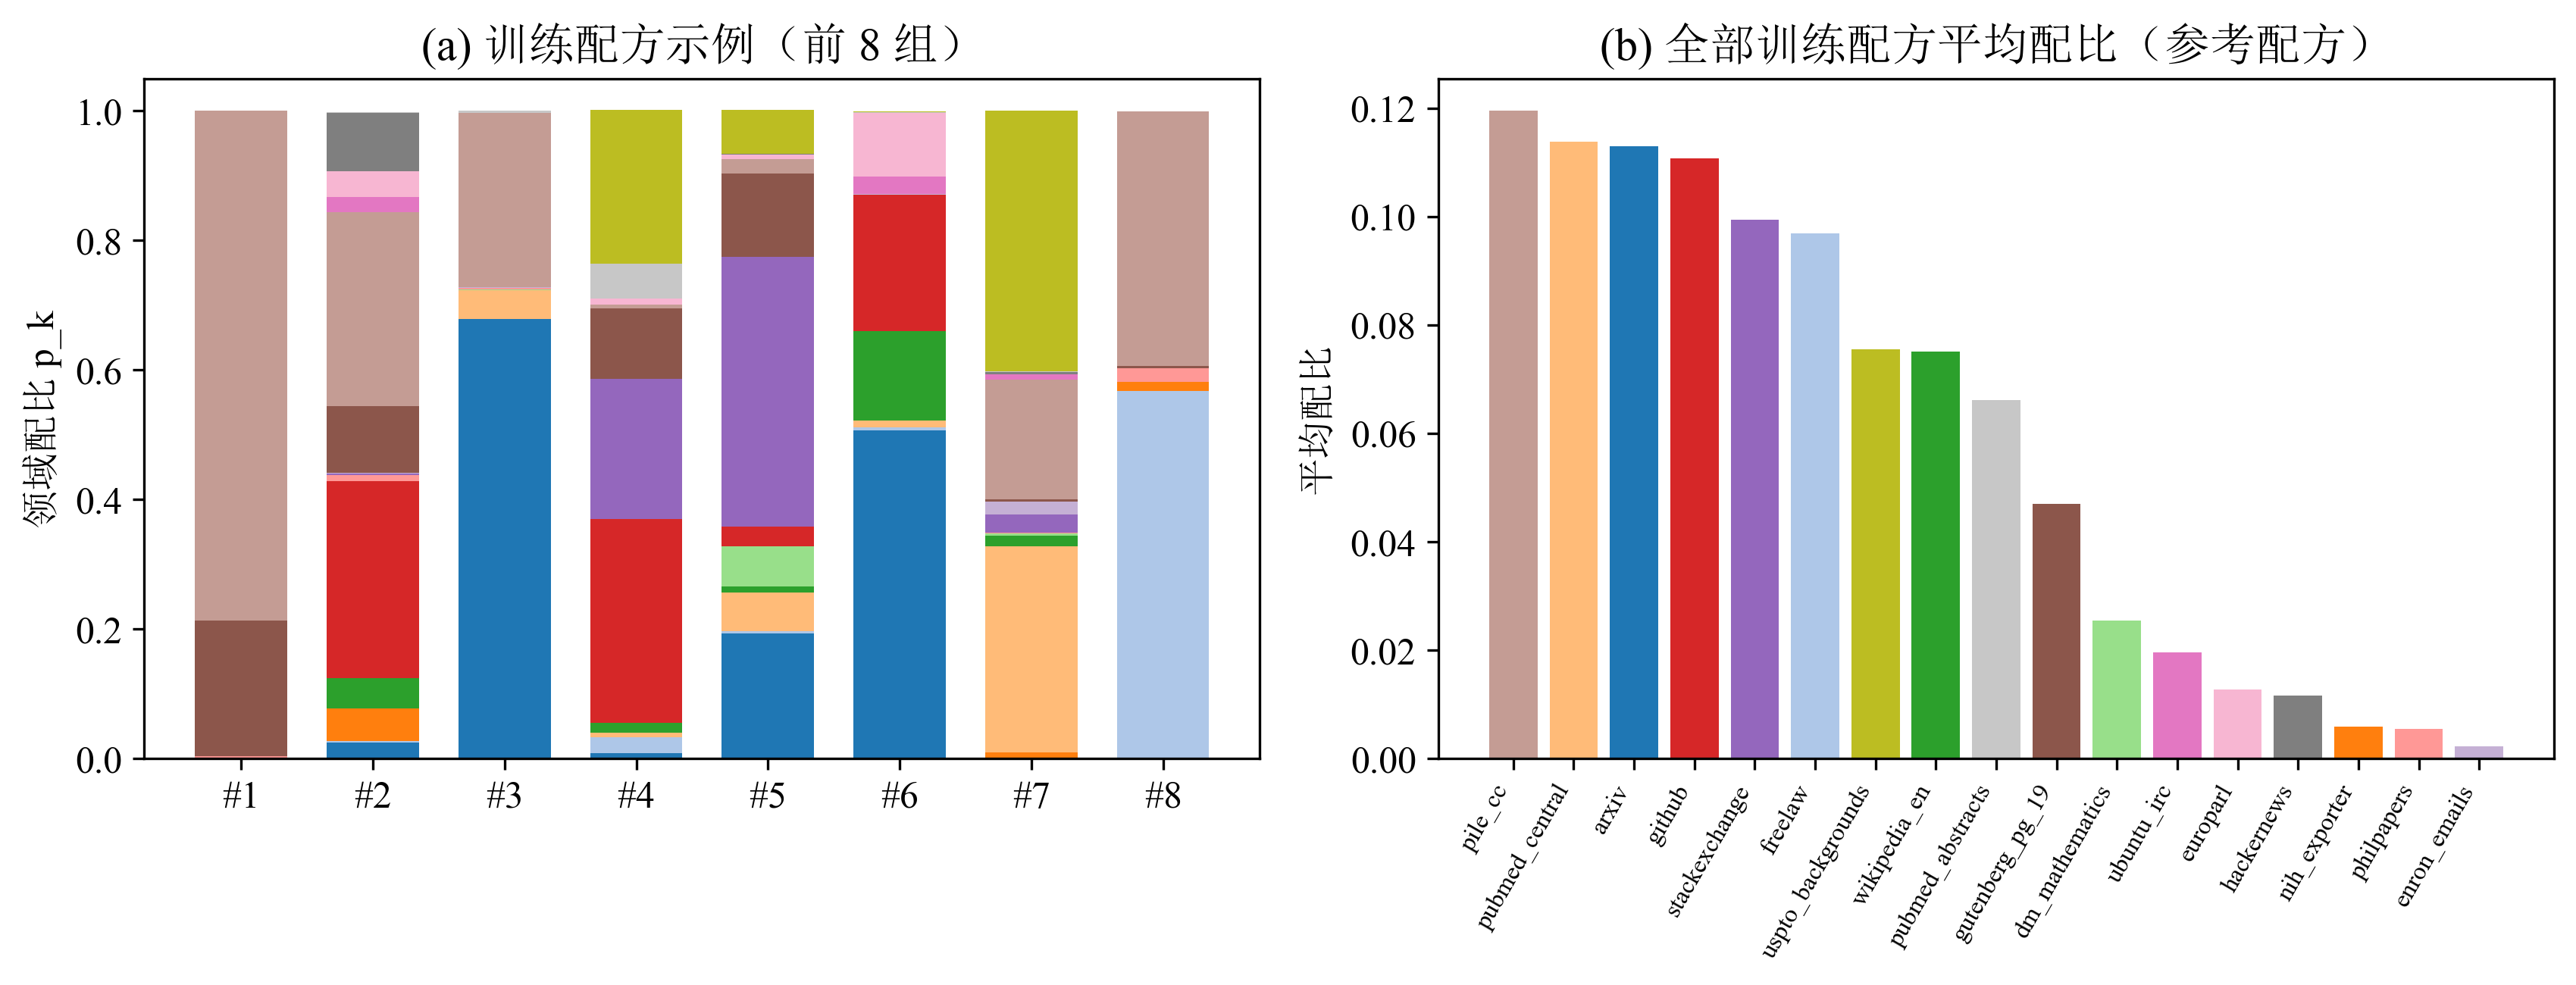
\includegraphics[width=0.92\textwidth]{求解/问题一/图片/图1_训练配比结构.png}
  \caption{训练配方结构（左：前 8 组配方堆叠；右：全部配方平均配比）}
  \label{fig:p1_structure}
\end{figure}

\begin{figure}[ht]
  \centering
  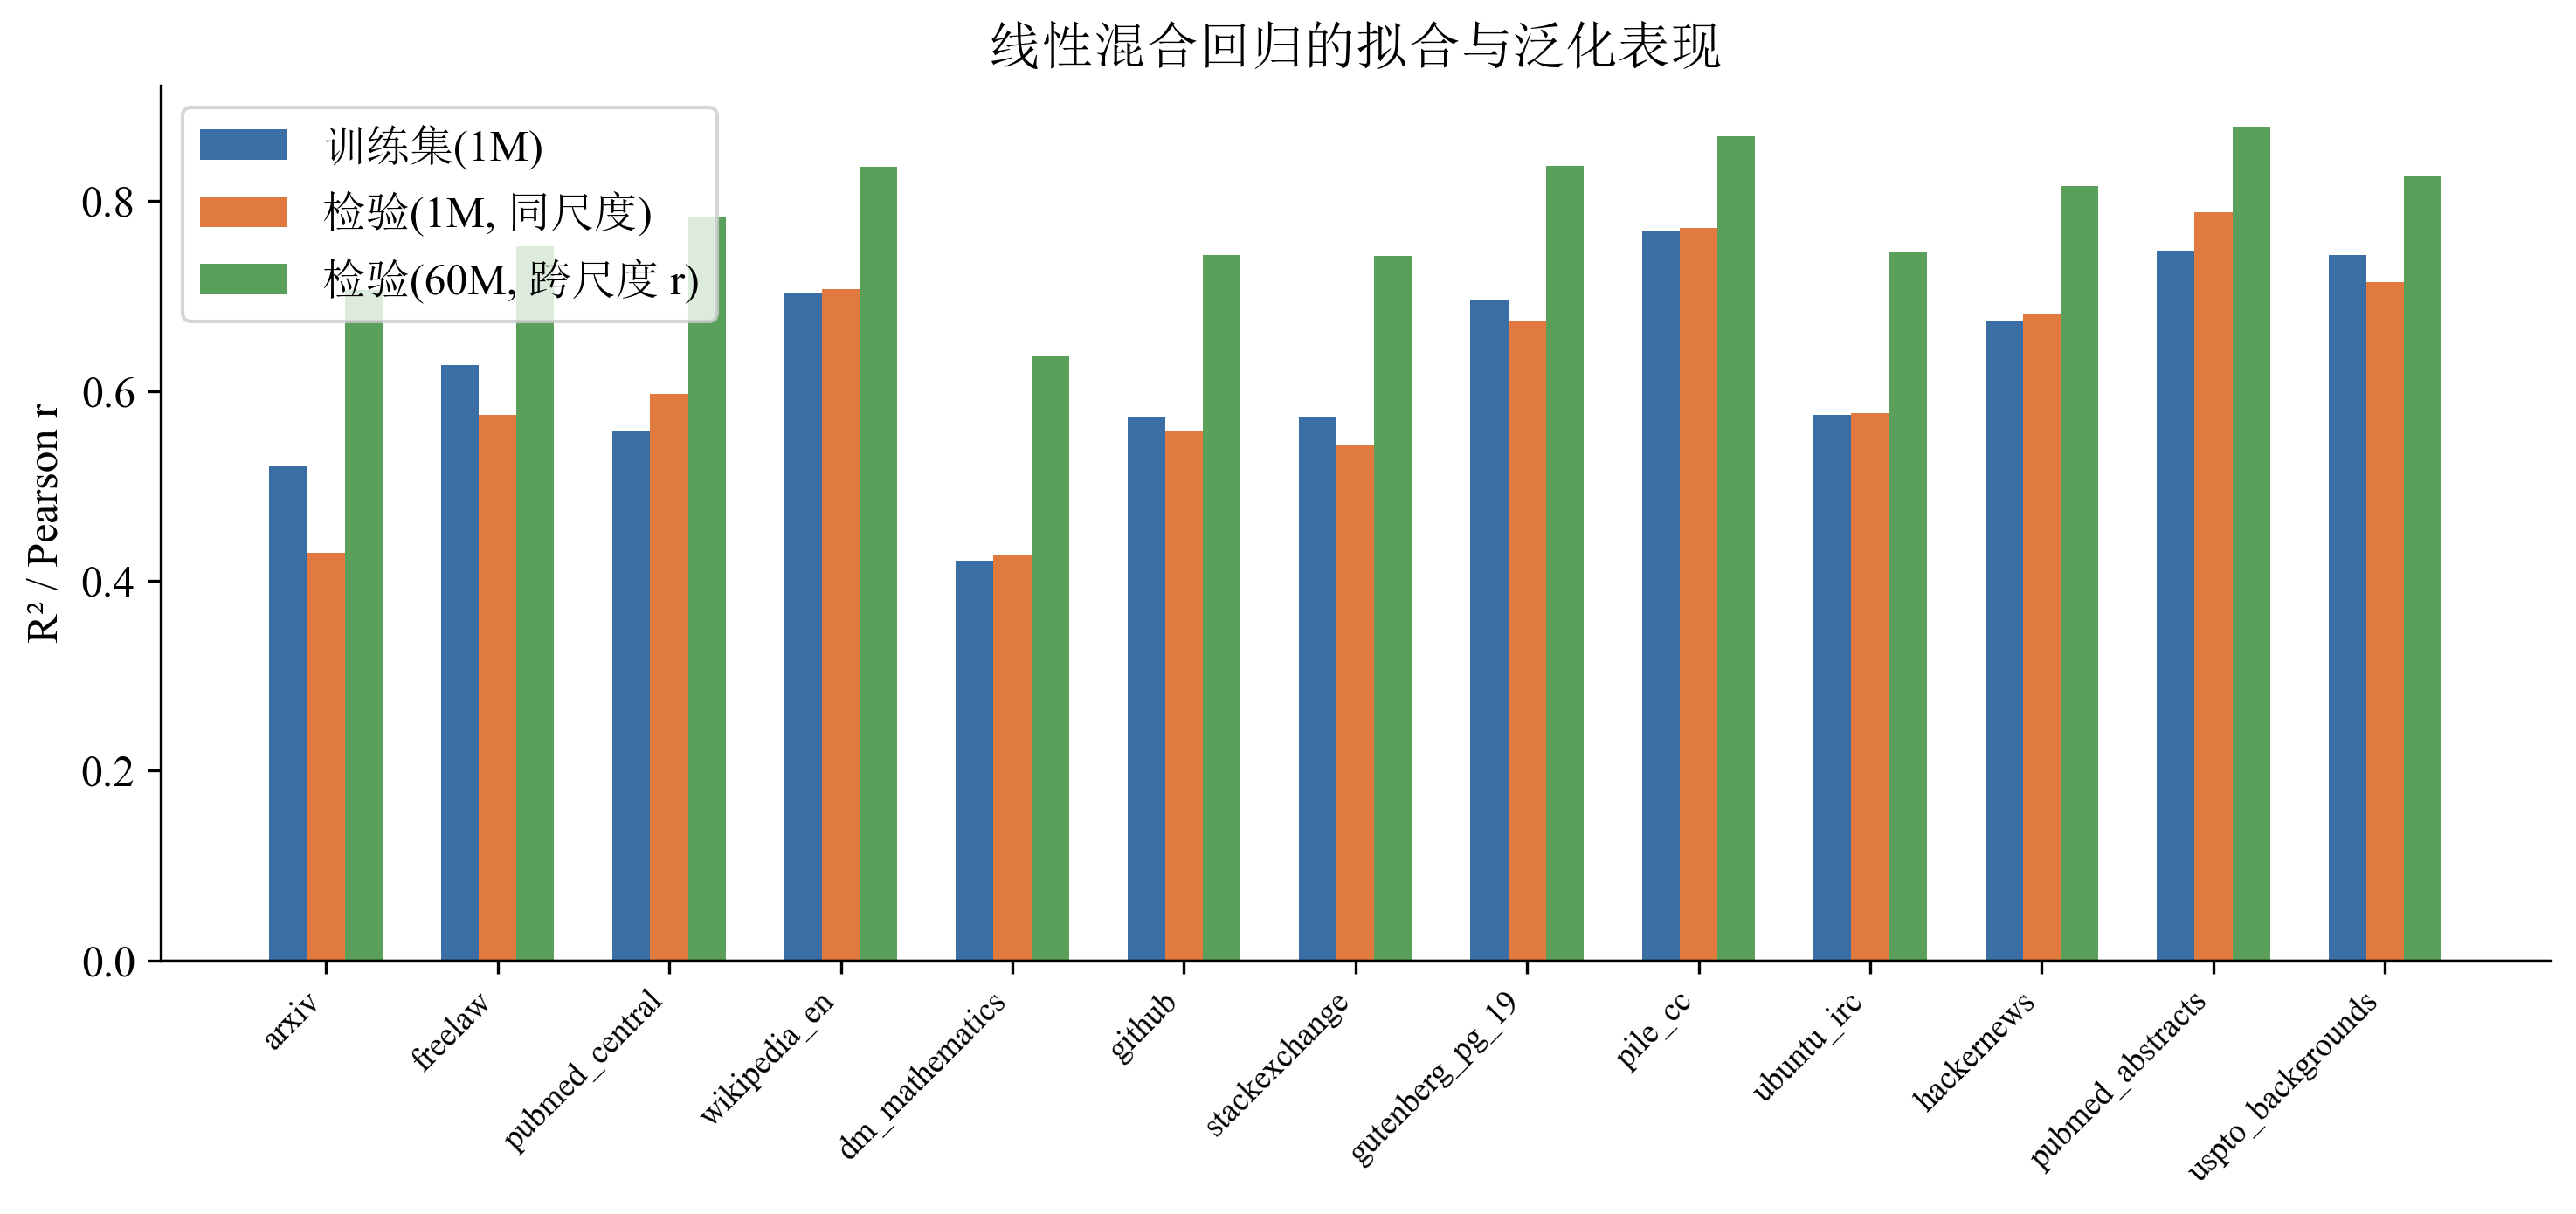
\includegraphics[width=0.72\textwidth]{求解/问题一/图片/图2_线性模型R2.png}
  \caption{线性混合回归的拟合与泛化表现}
  \label{fig:p1_r2}
\end{figure}

\begin{figure}[ht]
  \centering
  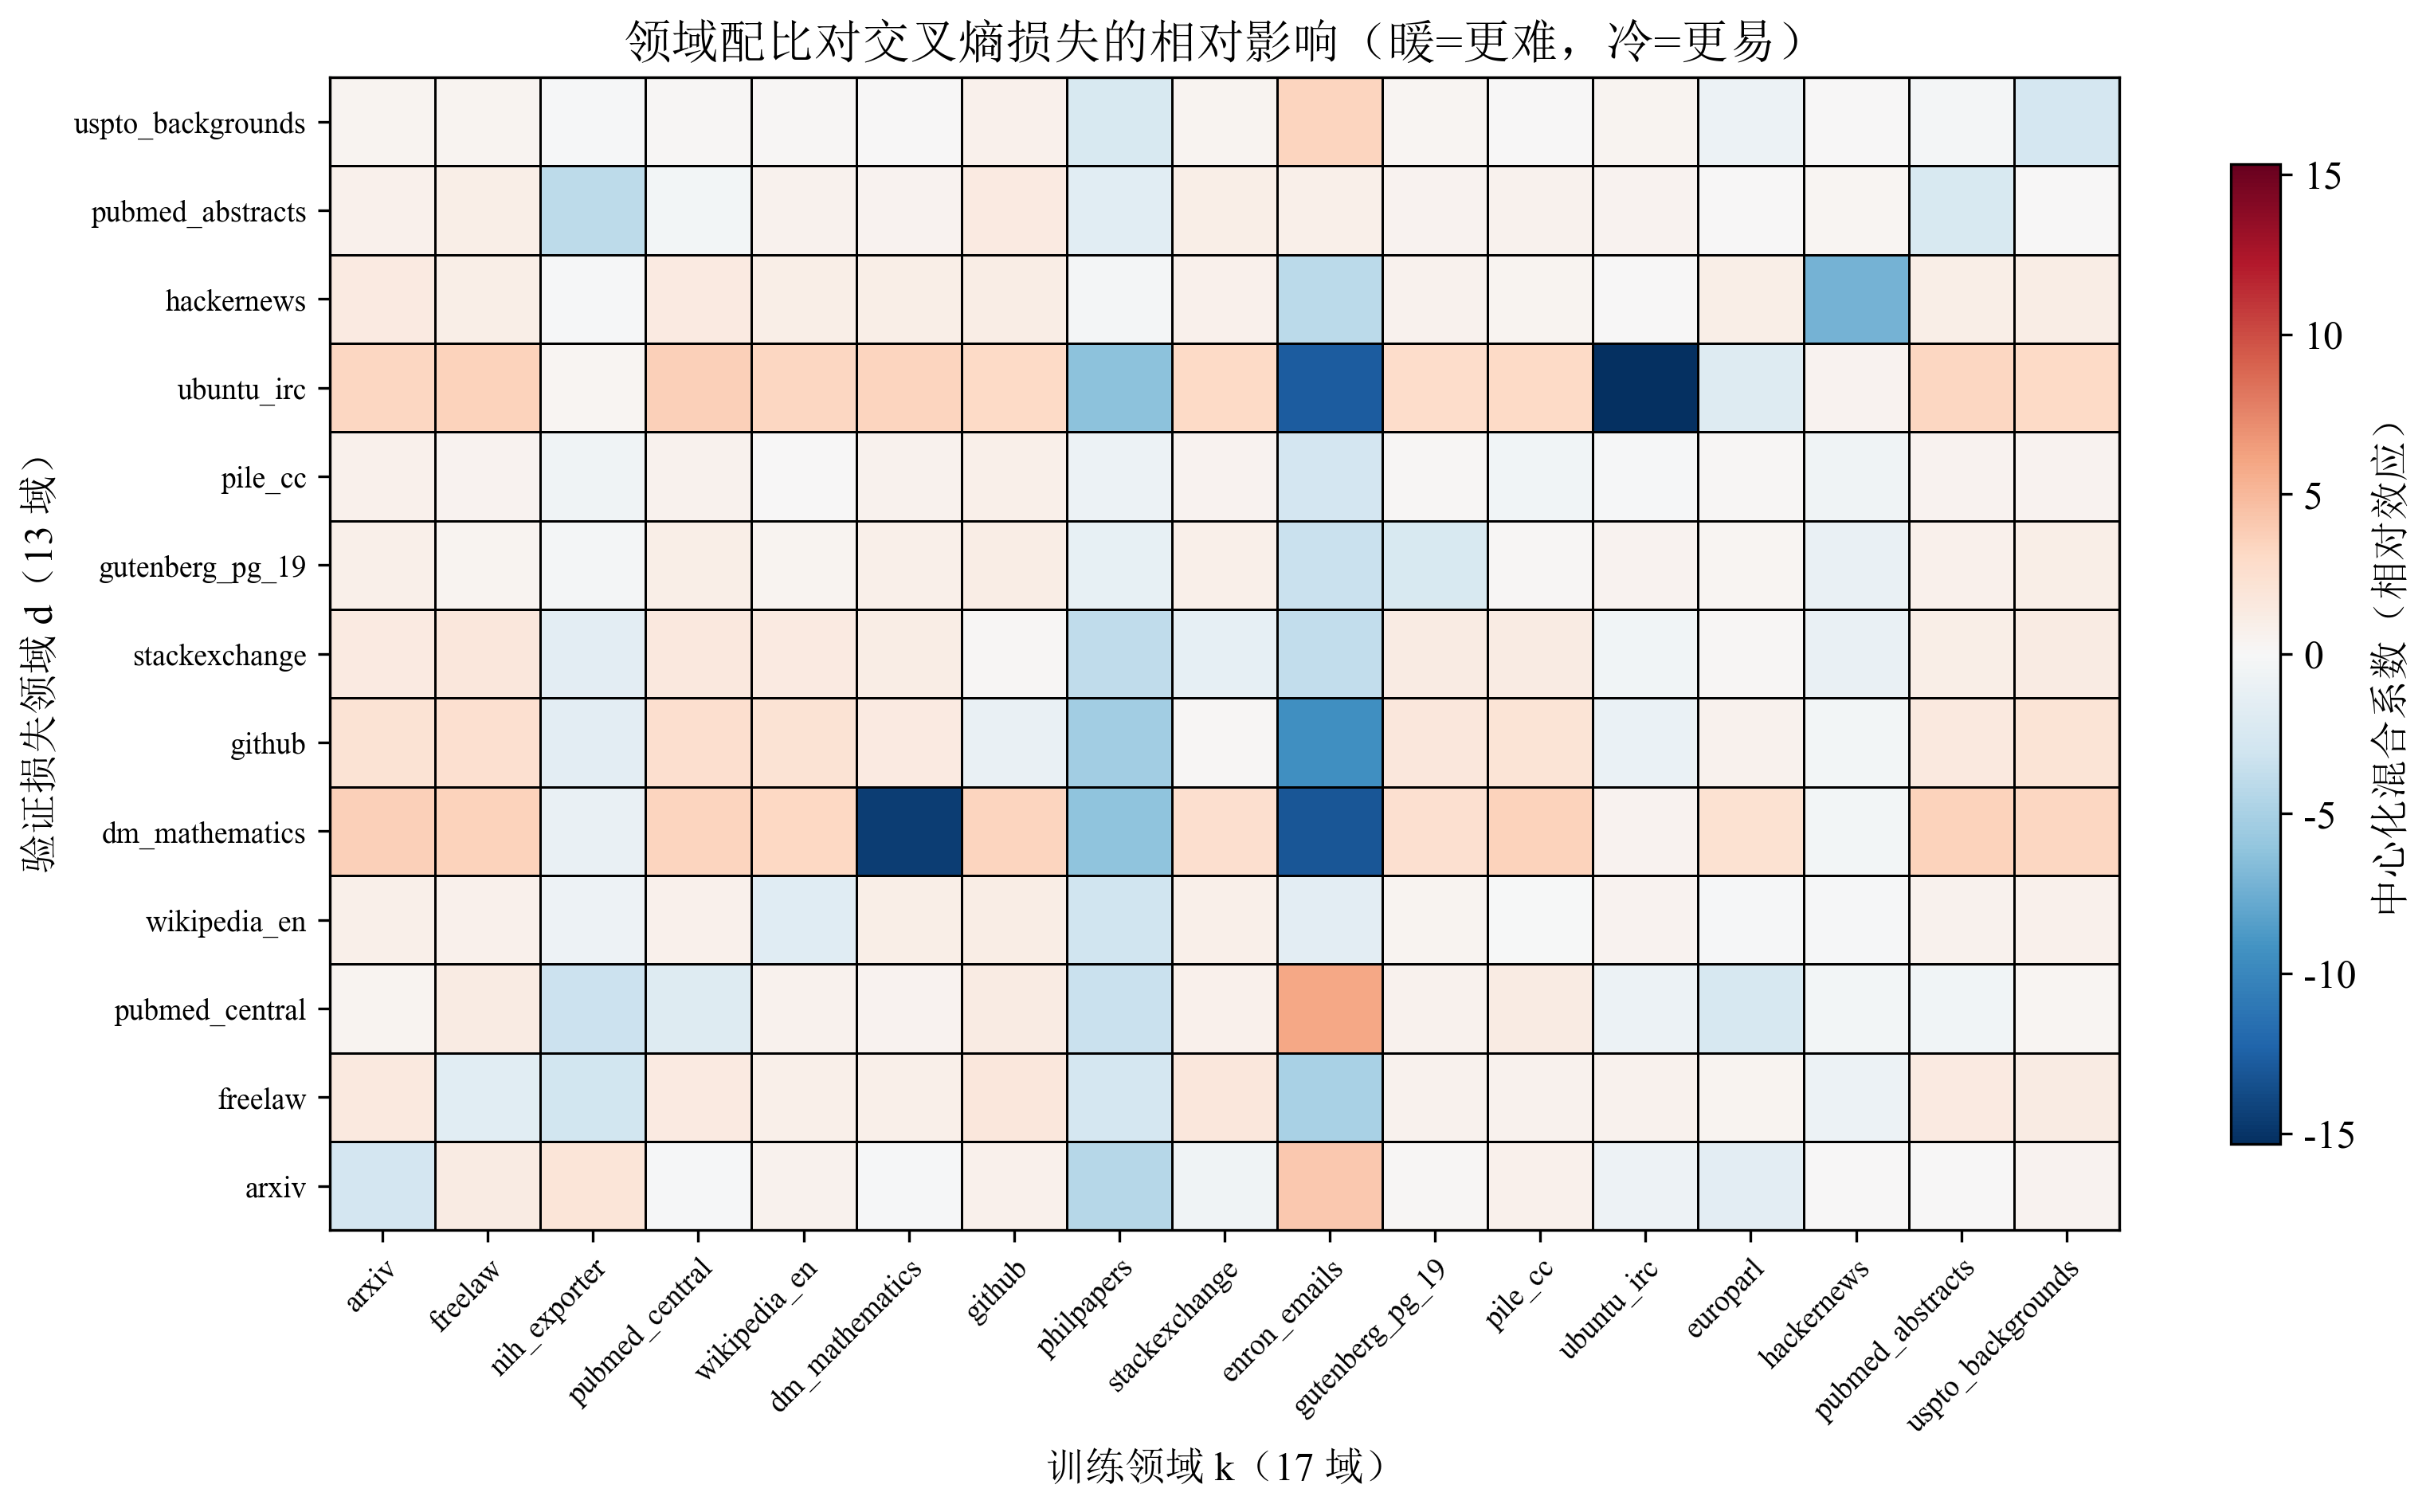
\includegraphics[width=0.78\textwidth]{求解/问题一/图片/图4_混合系数热力图.png}
  \caption{领域配比对交叉熵损失的相对影响热力图}
  \label{fig:p1_heatmap}
\end{figure}

\begin{figure}[ht]
  \centering
  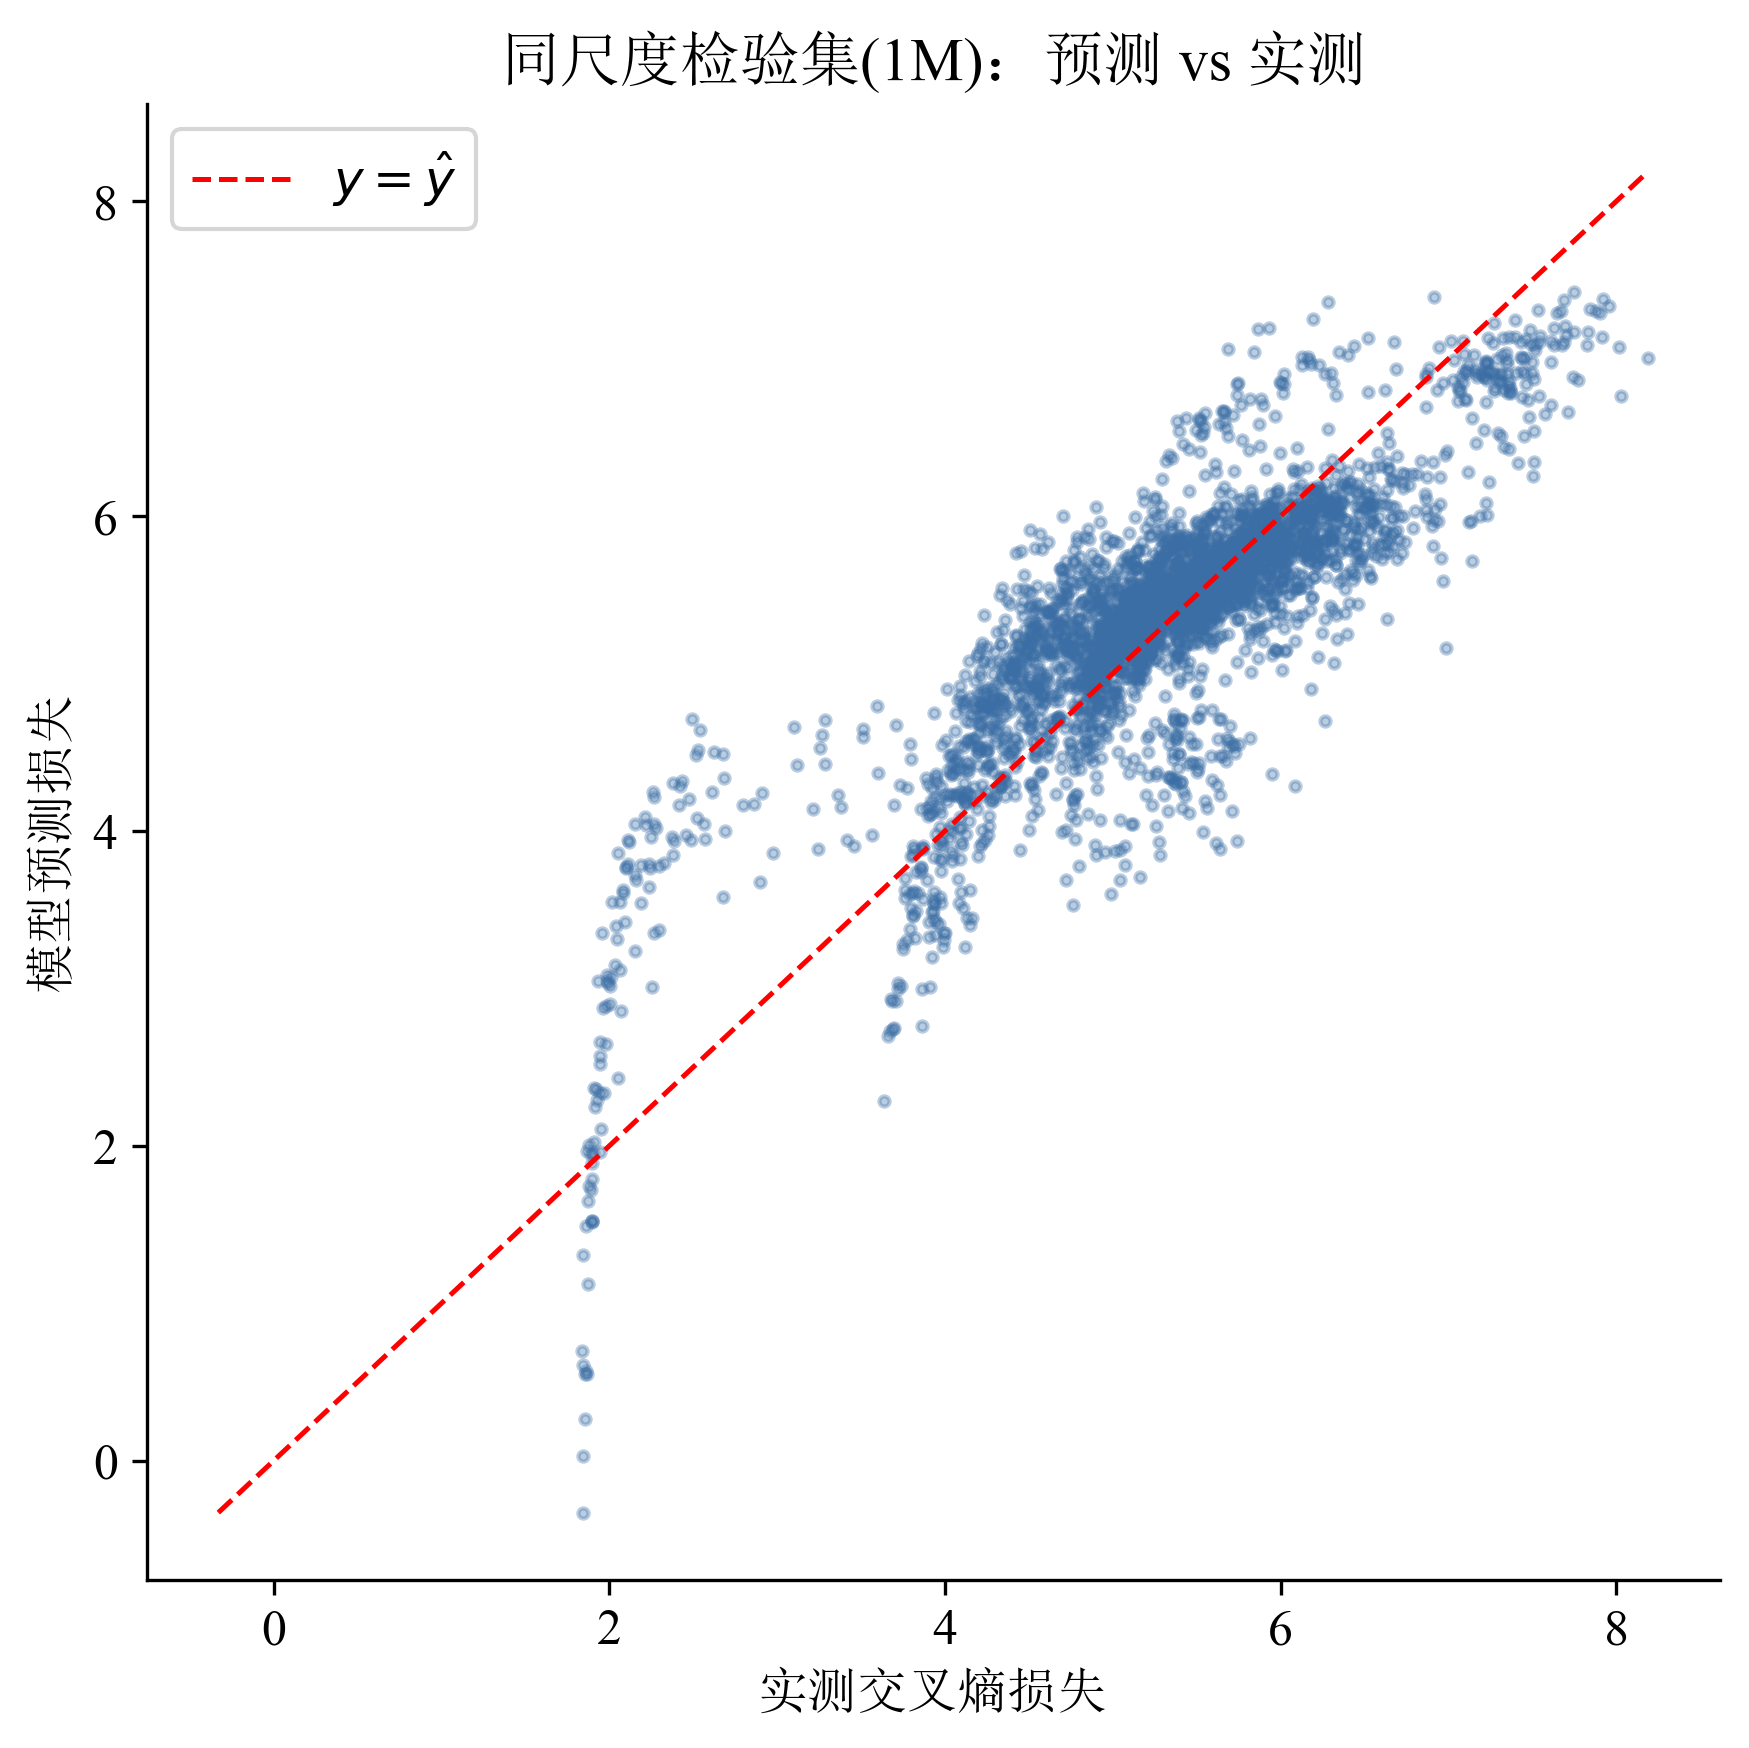
\includegraphics[width=0.58\textwidth]{求解/问题一/图片/图3_预测vs实测.png}
  \caption{同尺度检验集（1M）预测损失与实测损失对比}
  \label{fig:p1_scatter}
\end{figure}

由图\ref{fig:p1_r2}可知，训练集上 13 个损失域的 $R^2$ 位于 $0.42\sim0.77$ 之间、平均 $0.629$；同尺度 1M 检验集平均 $R^2=0.619$，与训练接近，说明模型未明显过拟合。由于不同参数规模下损失水平本身不同（60M 与 1M 的损失比约 $0.68$），跨尺度直接比较 $R^2$ 无意义，故改用尺度无关的 Pearson 相关：60M 与 1B 检验集上的平均相关分别为 $0.782$ 与 $0.651$，表明同一套配比—损失系数可在不同参数规模间复用。由图\ref{fig:p1_heatmap}可知，各训练域对验证损失的相对影响差异明显，dm\_mathematics、arxiv 等域降低损失，而 pile\_cc、ubuntu\_irc 等域抬高损失，印证了领域配比是影响模型性能的关键变量。

为验证质量信息的引入方式，本文比较了“仅配比”与“配比+混合质量指数 $\bar Q$”两种设定：追加质量项后 13 个损失域的平均 $R^2$ 增量仅为 $9.9\times10^{-5}$，说明线性配比系数已经吸收了质量信息。因此本文不把质量评分再次作为配比模型的解释变量，而是将其作为独立资源交由问题二、三使用。

两套质量口径（A1--A3 的熵权质量 $Q$ 与损失难度代理 $Q^{(\text{loss})}$）在 6 个可映射域上的排序一致性如图\ref{fig:p1_quality}所示。

\begin{figure}[ht]
  \centering
  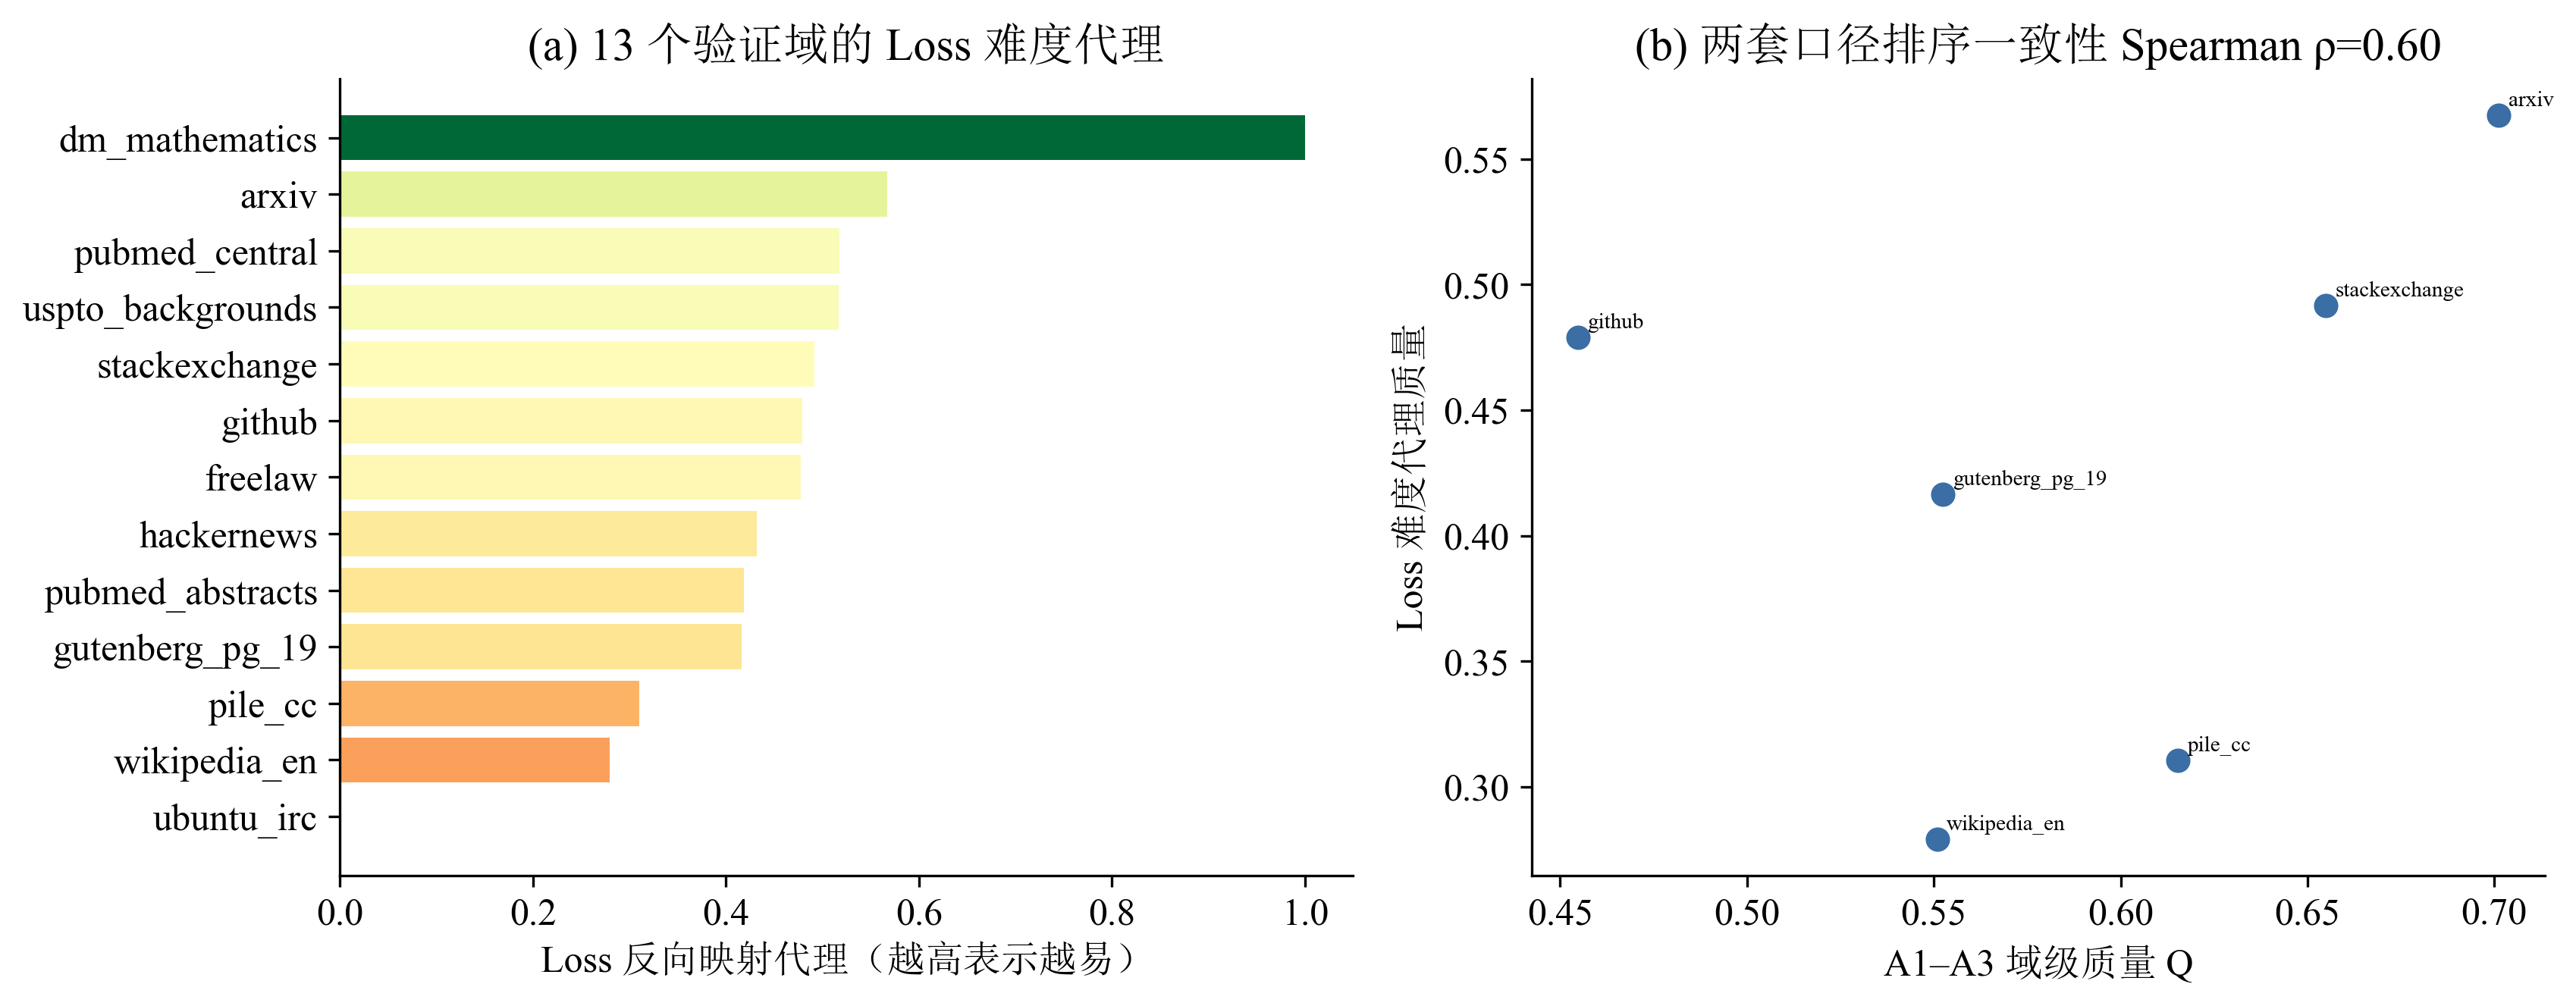
\includegraphics[width=0.92\textwidth]{求解/问题一/图片/图5_领域质量评分.png}
  \caption{左：13 个验证域的损失难度代理；右：A1--A3 质量与损失难度代理的排序一致性}
  \label{fig:p1_quality}
\end{figure}

由图\ref{fig:p1_quality}(a)可知，13 个损失域的内在难度差异显著，dm\_mathematics 最易（代理质量 $1.000$）、ubuntu\_irc 最难（代理质量 $0.000$）；图\ref{fig:p1_quality}(b)显示，A16 的 direct/near\_direct 映射中两套口径的 Spearman 排序相关为 $0.60$：arxiv、stackexchange、github 三个域在两种口径下同向（文本质量高、损失也相对低），但 wikipedia、book、pile\_cc 存在明显分歧——文本质量较高而该域损失并不低（学术与百科长文属“高质量但难拟合”）。因此质量评分必须按用途区分：面向数据治理使用 A1--A3 的文本质量，面向性能预测使用损失难度代理。

\textbf{3.最优配比与跨尺度稳健性}

无约束优化倾向于把配比集中于单一低损失域（预测加权平均损失 $4.177$），不具备可落地性；故采用 2.5 倍上限的有界推荐作为最终方案，推荐配比与参考配比的对比见表\ref{tab:p1_rec}，该方案使预测加权平均损失由 $5.336$ 降至 $5.136$（下降 $0.199$）。

\begin{longtable}{>{\centering\arraybackslash}p{0.30\textwidth}>{\centering\arraybackslash}p{0.22\textwidth}>{\centering\arraybackslash}p{0.22\textwidth}>{\centering\arraybackslash}p{0.20\textwidth}}
  \caption{有界推荐配比调整}
  \label{tab:p1_rec} \\
  \toprule
  领域 & 参考配比 & 推荐配比 & 调整量 \\
  \midrule
  \endfirsthead
  \caption{有界推荐配比调整（续）} \\
  \toprule
  领域 & 参考配比 & 推荐配比 & 调整量 \\
  \midrule
  \endhead
  \bottomrule
  \endfoot
  pubmed\_central & 0.1137 & 0.2843 & $+0.1706$ \\
  stackexchange & 0.0994 & 0.2486 & $+0.1491$ \\
  pubmed\_abstracts & 0.0662 & 0.1654 & $+0.0993$ \\
  gutenberg\_pg\_19 & 0.0469 & 0.1173 & $+0.0704$ \\
  dm\_mathematics & 0.0255 & 0.0637 & $+0.0382$ \\
  uspto\_backgrounds & 0.0755 & 0.0000 & $-0.0755$ \\
  freelaw & 0.0968 & 0.0000 & $-0.0968$ \\
  github & 0.1107 & 0.0000 & $-0.1107$ \\
  arxiv & 0.1130 & 0.0000 & $-0.1130$ \\
  pile\_cc & 0.1195 & 0.0000 & $-0.1195$ \\
\end{longtable}

由表\ref{tab:p1_rec}可知，推荐方案应显著增加 pubmed\_central、stackexchange、pubmed\_abstracts 等学术领域的配比，同时压缩 pile\_cc、arxiv、github、freelaw 等领域的占比。需要说明的是，这一结论是针对“13 个验证域加权平均损失”这一目标的优化结果，与“提升单个域自身表现”并不等价（例如 arxiv 的配比下降并不意味着 arxiv 质量低，而是因为其对加权平均损失的边际贡献为负）。外推稳健性方面，10B 与 70B 外推表的损失尺度因子（est/train）在各损失域上高度一致（10B 均值 $0.338$、标准差 $0.038$；70B 均值 $0.266$、标准差 $0.036$），且同配方下 60M 与 1M 的跨尺度损失比稳定（均值 $0.51\sim0.82$），说明同一套配比—损失系数可在不同参数规模间复用、具备跨尺度外推能力，如图\ref{fig:p1_extrap}所示。

\begin{figure}[ht]
  \centering
  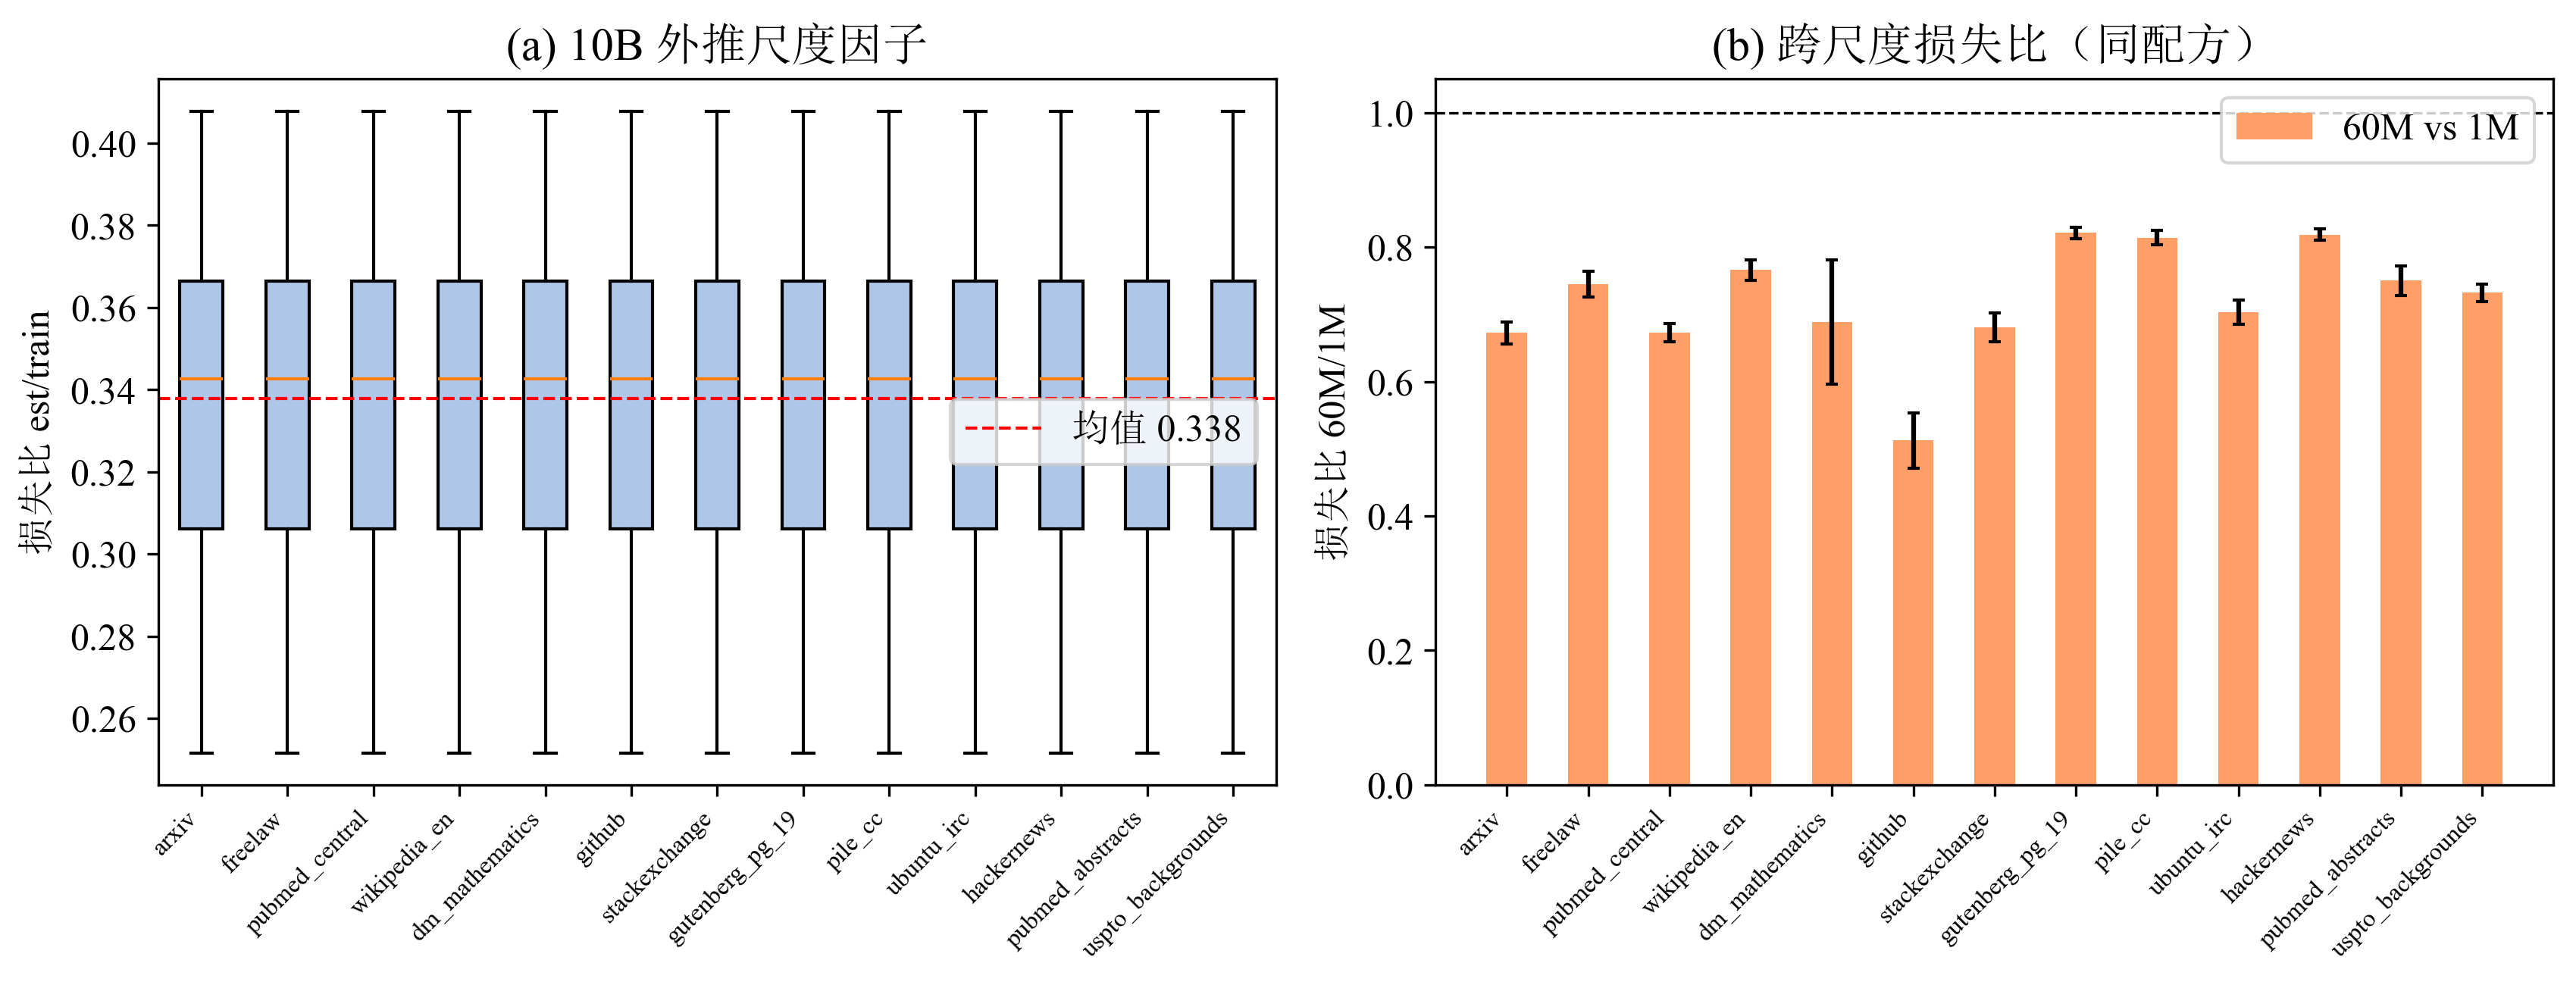
\includegraphics[width=0.92\textwidth]{求解/问题一/图片/图7_外推与跨尺度.png}
  \caption{外推稳健性验证（左：10B 外推尺度因子；右：同配方 60M/1M 跨尺度损失比）}
  \label{fig:p1_extrap}
\end{figure}

综合以上结果，本节完成了问题一的求解，得到领域质量评分 $Q$、最优配比 $\bm p$ 与配比—损失定量关系，为后续问题提供质量与配比输入。

\subsection{问题二的模型的建立和求解}

\subsubsection{具体分析}

针对问题二，本问属于\textbf{标度律建模与多元回归}类问题，需要完成四项递进任务：一是拟合只含参数规模 $N$ 与数据规模 $D$ 的经典标度律；二是对附件 B 的质量信号字段做方向检验，判断其是“质量”还是“难度/噪声”；三是将数据质量 $Q$ 与领域配比 $\bm p$ 纳入经典标度律，建立同时含 $N$、$D$、$Q$、$\bm p$ 的广义标度律\cite{muennighoff2023scaling}；四是分析各因素的边际效用与弹性，推导质量与参数规模相互替代的条件。本问综合采用稳健非线性最小二乘拟合经典 Chinchilla 标度律，采用控制变量组内相关检验判定质量字段方向，采用信息准则与内插外推表现比较四类广义标度律形式，并基于弹性分析与等损失曲线刻画质量—参数替代关系。

首先利用 Pythia 主拟合数据拟合 $L=E+A/N^{\alpha}+B/D^{\beta}$ 形式的经典标度律，并以“小模型训练、大模型留出”的方式检验参数可迁移性；接着在控制 $N$、$D$ 的组内条件下审计 $Q_{\text{score}}$ 与损失的相关方向，据此确定质量定义；然后将 Pythia 与半合成质量数据联合拟合，比较四种质量项形式并择优；最后计算各因素弹性与等损失曲线，给出“提升数据质量等价于增加多少参数量”的替代率，并用问题一的配比系数刻画领域间的替代与互补结构。

\subsubsection{模型准备}

\textbf{1.数据预处理}

本问数据来自附件 B：B1 为 Pythia 系列模型在多个参数规模下的训练损失轨迹（1{,}176 点，8 个模型 $\times$ 147 个检查点）\cite{biderman2023pythia}；B2 为 Cerebras 半合成轨迹；B3 为 8 条 Pythia 插值轨迹（8$\times$500）；B4 为 12 个模型族的跨族收敛点；B5 为已发表标度律数据；B6/B7 为含 $Q_{\text{score}}$ 的半合成质量实验；B8 为大规模矩阵（含外推段）；B9/B10 为百亿参数以上的模型元数据与预估损失。经典标度律以 $N$（参数量，B）与 $D$（训练数据量，B tokens）为自变量、验证损失 $L$ 为因变量；广义标度律进一步引入质量 $Q$。由于 $N$、$D$ 均跨多个数量级，拟合一律在原函数上进行（而非双对数线性化），以保留不可约损失 $E$ 的常数项结构。

\textbf{2.质量字段方向审计}

附件 B 的 $Q_{\text{score}}$ 字段语义未在数据说明中给出，必须先判定方向。判据是：在控制 $N$、$D$ 相同（即同一 $(N,D)$ 分组内）的前提下，若 $Q_{\text{score}}$ 与损失显著正相关，则其为“难度/噪声比例”，须取补变换；若显著负相关，则其本身即为“质量”指标。审计结果如表\ref{tab:p2_dir}所示。

\begin{longtable}{>{\centering\arraybackslash}p{0.18\textwidth}>{\centering\arraybackslash}p{0.10\textwidth}>{\centering\arraybackslash}p{0.12\textwidth}>{\centering\arraybackslash}p{0.16\textwidth}>{\raggedright\arraybackslash}p{0.36\textwidth}}
  \caption{质量字段 $Q_{\text{score}}$ 的方向审计（控制 $N$、$D$ 的组内相关）}
  \label{tab:p2_dir} \\
  \toprule
  数据集 & 样本数 & 分组数 & 组内相关 $r$ & 结论 \\
  \midrule
  \endfirsthead
  \caption{质量字段方向审计（续）} \\
  \toprule
  数据集 & 样本数 & 分组数 & 组内相关 $r$ & 结论 \\
  \midrule
  \endhead
  \bottomrule
  \endfoot
  B6 & 360 & 45 & $-0.925$ & $Q$ 越大损失越低：\textbf{质量指标}（$Q=1$ 为最优） \\
  B7 & 450 & 45 & $-0.918$ & 与 B6 一致，可作独立验证 \\
  B8（校准段） & 984 & 90 & $+0.995$ & 方向与 B6/B7 相反：\textbf{口径不一致} \\
  B8（外推段） & 720 & 60 & $+0.968$ & 同上 \\
\end{longtable}

由表\ref{tab:p2_dir}可知，B6 与 B7 独立地给出 $-0.925$ 与 $-0.918$ 的组内相关，可确认 $Q_{\text{score}}$ 就是数据质量（越高越好），故取 $Q=Q_{\text{score}}$，与问题一“越高越好”的口径一致。但 B8 的两个子集给出相反符号（$+0.995$、$+0.968$），且其最小损失（$0.50$）低于由 Pythia 标定的不可约损失 $E$，说明 B8 与 B6/B7 使用了不同的质量口径（或将质量定义反号），**不能并入拟合**；本文仅在其方向重定向（取 $1-Q_{\text{score}}$）后作一致性检验，并据此明确标注半合成数据的可信度边界。

\textbf{3.算法选择}

本问涉及经典标度律拟合、字段方向检验与广义标度律建模三类任务。经典标度律比较双对数线性回归与非线性最小二乘：前者忽略常数项 $E$ 会引入偏置，故采用带界约束的非线性最小二乘直接拟合原函数，并使用 soft-$L_1$ 稳健损失以降低个别检查点的杠杆效应。方向检验采用控制 $(N,D)$ 的组内相关，可剔除规模与数据量的混杂。广义标度律对四种候选形式做同口径比较，评价指标为联合拟合优度、B6 内部拟合优度、B7 新增点外推相关与 AIC，结果如表\ref{tab:p2_form}所示。

\begin{longtable}{>{\centering\arraybackslash}p{0.28\textwidth}>{\centering\arraybackslash}p{0.13\textwidth}>{\centering\arraybackslash}p{0.13\textwidth}>{\centering\arraybackslash}p{0.13\textwidth}>{\centering\arraybackslash}p{0.10\textwidth}>{\centering\arraybackslash}p{0.13\textwidth}}
  \caption{广义标度律候选形式的比较}
  \label{tab:p2_form} \\
  \toprule
  质量项形式 & 联合 $R^2$ & B6 拟合 $R^2$ & B7 新增点 $r$ & 参数数 & AIC \\
  \midrule
  \endfirsthead
  \caption{广义标度律候选形式的比较（续）} \\
  \toprule
  质量项形式 & 联合 $R^2$ & B6 拟合 $R^2$ & B7 新增点 $r$ & 参数数 & AIC \\
  \midrule
  \endhead
  \bottomrule
  \endfoot
  \textbf{加性质量缺口 $C(1-Q)^{\gamma}$} & \textbf{0.9896} & \textbf{0.9556} & 0.991 & 7 & $\mathbf{-10236}$ \\
  质量同时乘 $N$ 与 $D$ & 0.9882 & 0.9495 & \textbf{0.991} & 7 & $-10042$ \\
  加性质量亏损 $CQ^{-\gamma}$ & 0.9848 & 0.9349 & 0.991 & 7 & $-9660$ \\
  质量作有效数据乘子 & 0.9745 & 0.8905 & 0.983 & 6 & $-8866$ \\
\end{longtable}

如表\ref{tab:p2_form}所示，四类形式的 B7 新增点外推相关均不低于 $0.983$，说明质量效应稳健存在；其中加性质量缺口形式在联合拟合、B6 内部拟合与 AIC 上均最优，故最终采用该形式。

\subsubsection{模型建立}

\textbf{步骤1：经典标度律模型}

以 Chinchilla 标度律为基础，验证损失 $L$ 满足：
\begin{equation}
    L(N,D) = E + \frac{A}{N^{\alpha}} + \frac{B}{D^{\beta}}
\end{equation}
其中 $E$ 为不可约损失（$N,D\to\infty$ 时的极限），$A/\alpha$ 刻画参数规模的边际收益，$B/\beta$ 刻画数据规模的边际收益。该模型隐含“数据质量取参考水平”的基线假设。

\textbf{步骤2：广义标度律模型}

将质量项以“质量缺口”形式引入，得到广义标度律：
\begin{equation}
    L(N,D,Q) = E + \frac{A}{N^{\alpha}} + \frac{B}{D^{\beta}} + C\,(1-Q)^{\gamma},
    \qquad C>0,\ \gamma>0
\end{equation}
该形式满足题设的自然设计要求：当数据质量达到完美（$Q=1$）时质量缺口项自动消失，模型精确退化为经典 Chinchilla 形式，与既有标度律完全兼容；同时其物理含义清晰——**数据质量决定了可达的不可约损失下限**：
\begin{equation}
    \lim_{N,D\to\infty} L(N,D,Q) = E + C\,(1-Q)^{\gamma} \;\ge\; E
\end{equation}
即无论投入多少算力，劣质语料都无法被规模弥补；反之质量越高，损失下限越低。该形式还避开了“加性质量增益 $E-CQ^{\gamma}$”在 $Q\to1$ 时使损失降到 $E-C<0$ 的非物理缺陷。

\textbf{步骤3：边际效用与弹性分析}

在参考点 $(N_0,D_0,Q_0)$ 处，各因素的边际效用为：
\begin{equation}
    \frac{\partial L}{\partial N} = -\alpha A N^{-\alpha-1},\quad
    \frac{\partial L}{\partial D} = -\beta B D^{-\beta-1},\quad
    \frac{\partial L}{\partial Q} = -\gamma C (1-Q)^{\gamma-1}
\end{equation}
对应弹性为：
\begin{equation}
    \varepsilon_N = \frac{\partial L}{\partial N}\frac{N_0}{L_0},\qquad
    \varepsilon_D = \frac{\partial L}{\partial D}\frac{D_0}{L_0},\qquad
    \varepsilon_Q = \frac{\partial L}{\partial Q}\frac{Q_0}{L_0}
\end{equation}

\textbf{步骤4：质量—参数替代条件}

设质量提升 $\mathrm dQ$ 带来的损失下降等于参数增加 $\mathrm dN$ 带来的损失下降，由等损失条件 $\mathrm dL=0$ 得：
\begin{equation}
    \left|\frac{\partial L}{\partial Q}\right|\mathrm dQ = \left|\frac{\partial L}{\partial N}\right|\mathrm dN
    \quad\Longrightarrow\quad
    \frac{\mathrm dN}{\mathrm dQ} = \frac{\gamma C (1-Q)^{\gamma-1}}{\alpha A N^{-\alpha-1}}
    = \frac{\gamma C}{\alpha A}\,(1-Q)^{\gamma-1}N^{\alpha+1}
\end{equation}
该替代率随 $N^{\alpha+1}$ 增长，说明**模型规模越大，参数扩张的边际效用越低，“以质量换规模”越划算**，这正是问题三在算力约束下权衡质量投入与规模投入的核心依据。

\textbf{步骤5：领域间的替代与互补}

线性混合模型下两个训练域 $i$、$j$ 对 13 个验证域损失的效应向量分别为 $\bm a_i,\bm a_j$，定义二者的可替代度为
\begin{equation}
    s_{ij} = \frac{\langle \bm a_i-\bar{\bm a},\ \bm a_j-\bar{\bm a}\rangle}{\|\bm a_i-\bar{\bm a}\|\,\|\bm a_j-\bar{\bm a}\|}
\end{equation}
其中 $\bar{\bm a}$ 为 17 个域的平均效应向量。$s_{ij}\to1$ 表示两域作用方式趋同、可在配比中相互替代；$s_{ij}\to-1$ 表示作用方式相反、构成互补（需搭配使用）。

\subsubsection{模型求解}

\textbf{1.经典标度律拟合与留出验证}

经典标度律在 B1 全量 1{,}176 点上的拟合结果如图\ref{fig:p2_classic}所示，参数估计如下：
\begin{equation}
    L(N,D) = 1.6898 + \frac{0.3540}{N^{0.3400}} + \frac{1.2403}{D^{0.2799}}
\end{equation}
拟合 $R^2 = 0.9999998$、RMSE $=1.5\times10^{-4}$、MAPE $=0.004\%$。以 4 个最小模型训练、预测其余 4 个更大模型，留出 $R^2$ 仍为 $0.9999997$、MAPE $=0.005\%$，说明标度律参数在模型族内部可迁移。

\begin{figure}[ht]
  \centering
  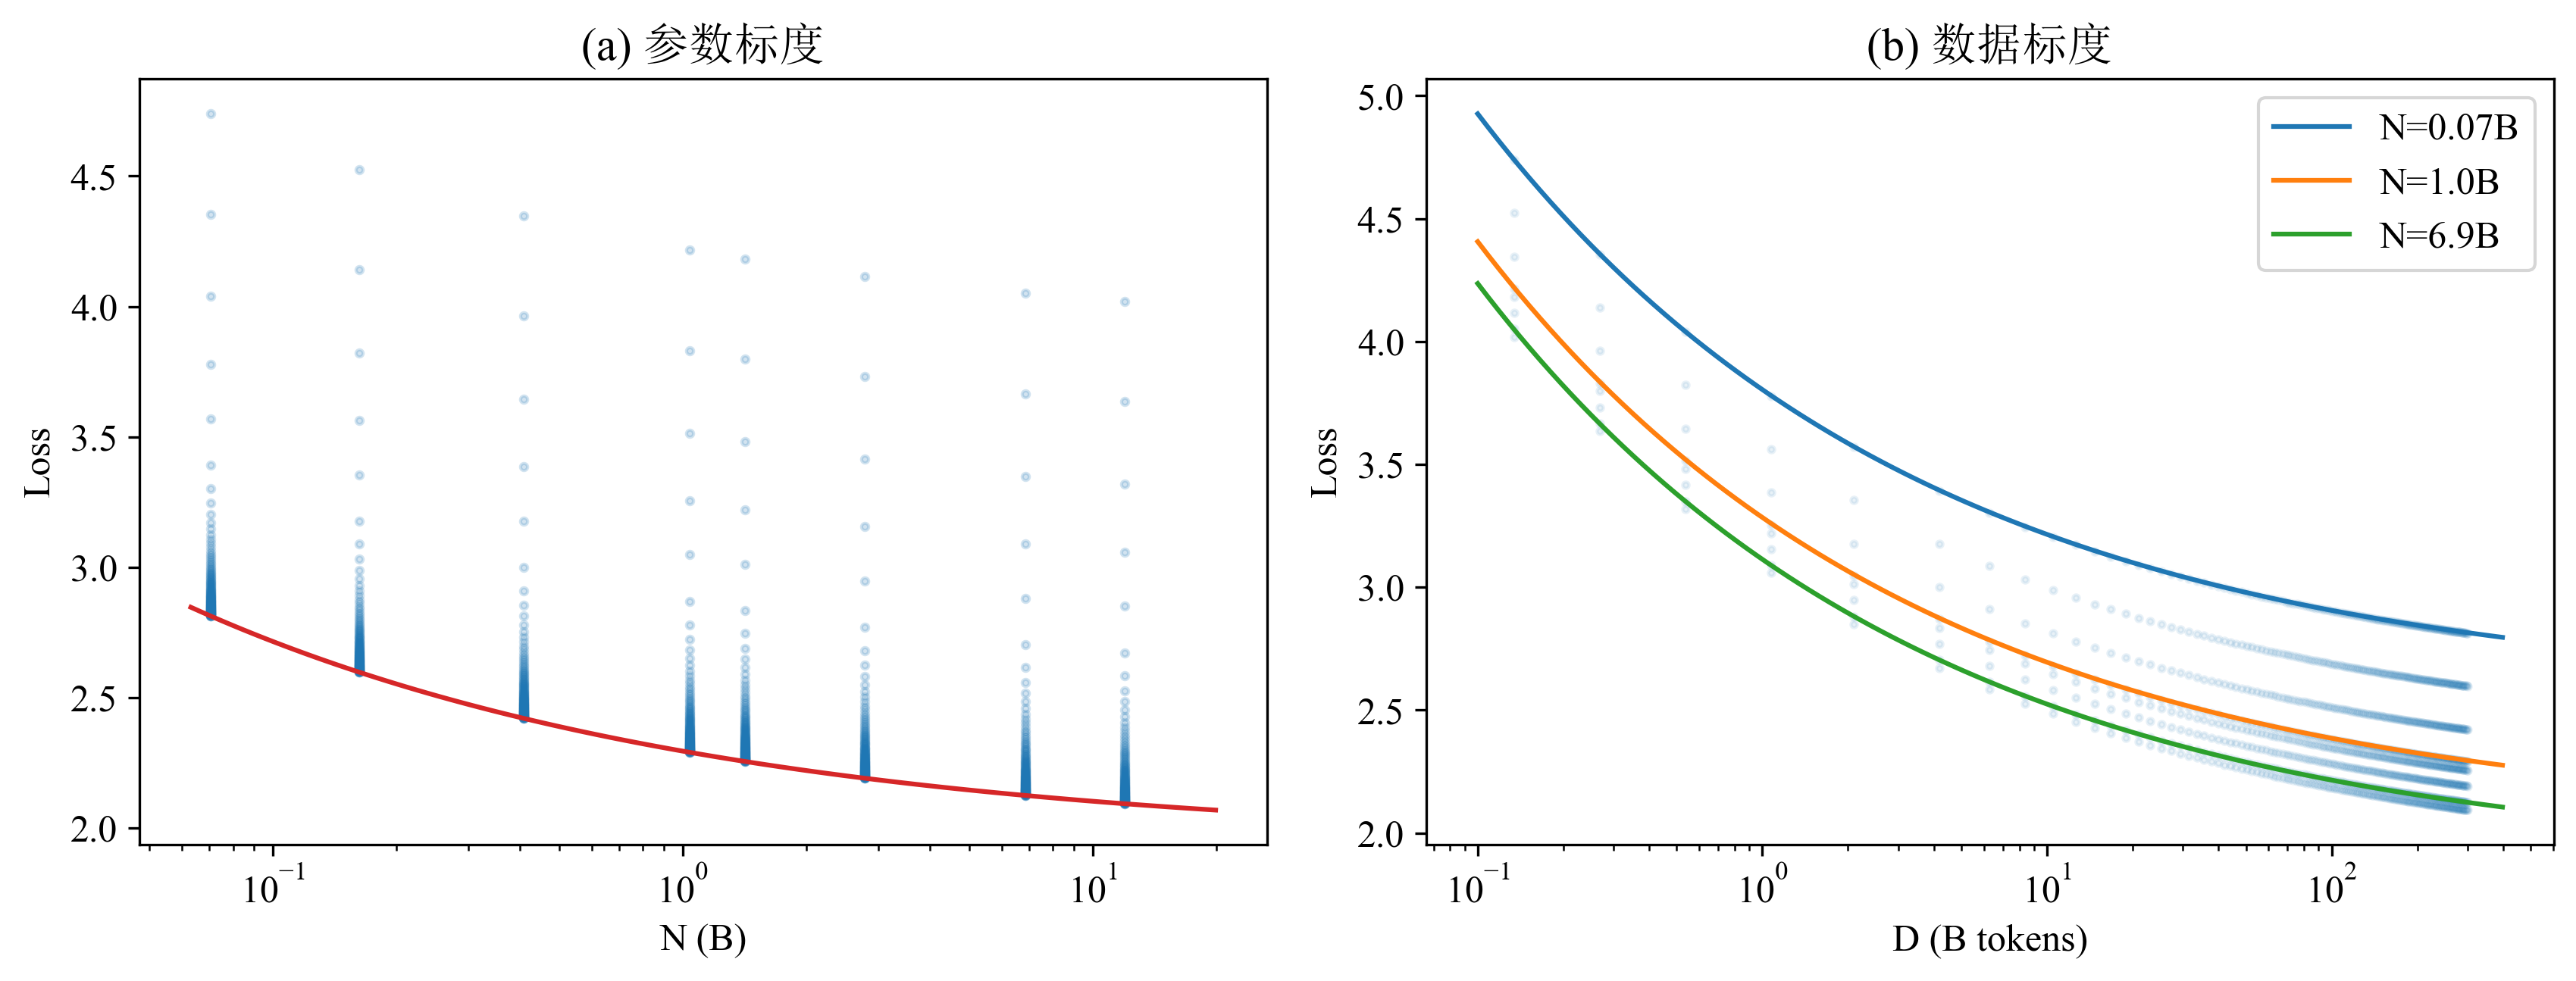
\includegraphics[width=0.92\textwidth]{求解/问题二/图片/图1_经典标度律拟合.png}
  \caption{经典标度律对 Pythia 训练轨迹的拟合（左：随参数规模；右：随数据规模）}
  \label{fig:p2_classic}
\end{figure}

需要客观指出：B1 拟合残差的标准差仅 $1.5\times10^{-4}$，而损失本身的标准差为 $0.342$，即该附件的损失值几乎是 $(N,D)$ 的无噪声函数。因此 B1 上的极高 $R^2$ 只能证明 Chinchilla 函数形式与数据自洽，**不能替代外部验证**；真实泛化能力必须由 B2/B4/B5 等独立来源检验（见本节第 3 部分）。

\textbf{2.广义标度律参数估计}

将 Pythia（无质量信息，取参考质量 $Q=1$）与 B6 质量实验联合拟合，采用表\ref{tab:p2_form}选定的加性质量缺口形式，参数估计如表\ref{tab:p2_params}所示。

\begin{longtable}{>{\centering\arraybackslash}p{0.30\textwidth}>{\centering\arraybackslash}p{0.18\textwidth}>{\centering\arraybackslash}p{0.20\textwidth}>{\raggedright\arraybackslash}p{0.24\textwidth}}
  \caption{广义标度律参数估计}
  \label{tab:p2_params} \\
  \toprule
  参数 & 估计值 & 参数 & 估计值 \\
  \midrule
  \endfirsthead
  \caption{广义标度律参数估计（续）} \\
  \toprule
  参数 & 估计值 & 参数 & 估计值 \\
  \midrule
  \endhead
  \bottomrule
  \endfoot
  不可约损失 $E$ & 1.6558 & 数据规模指数 $\beta$ & 0.2767 \\
  规模系数 $A$ & 0.3808 & 质量缺口系数 $C$ & 0.3544 \\
  规模指数 $\alpha$ & 0.3266 & 质量指数 $\gamma$ & 0.9779 \\
  数据系数 $B$ & 1.2515 & 联合拟合 $R^2$ & 0.9896 \\
\end{longtable}

由表\ref{tab:p2_params}可知，质量指数 $\gamma=0.9779\approx1$，说明质量缺口近似线性地压低损失下限；联合拟合 $R^2=0.9896$、RMSE $=0.036$、MAPE $=0.66\%$，引入质量项后并未牺牲拟合精度。质量缺口对损失的影响如图\ref{fig:p2_quality}所示，质量对损失下限的决定作用可由式 $E+C(1-Q)^{\gamma}$ 直接读出：当 $Q=1$ 时下限为 $1.656$，$Q=0.6$ 时为 $1.802$，$Q=0.3$ 时为 $2.135$。

\begin{figure}[ht]
  \centering
  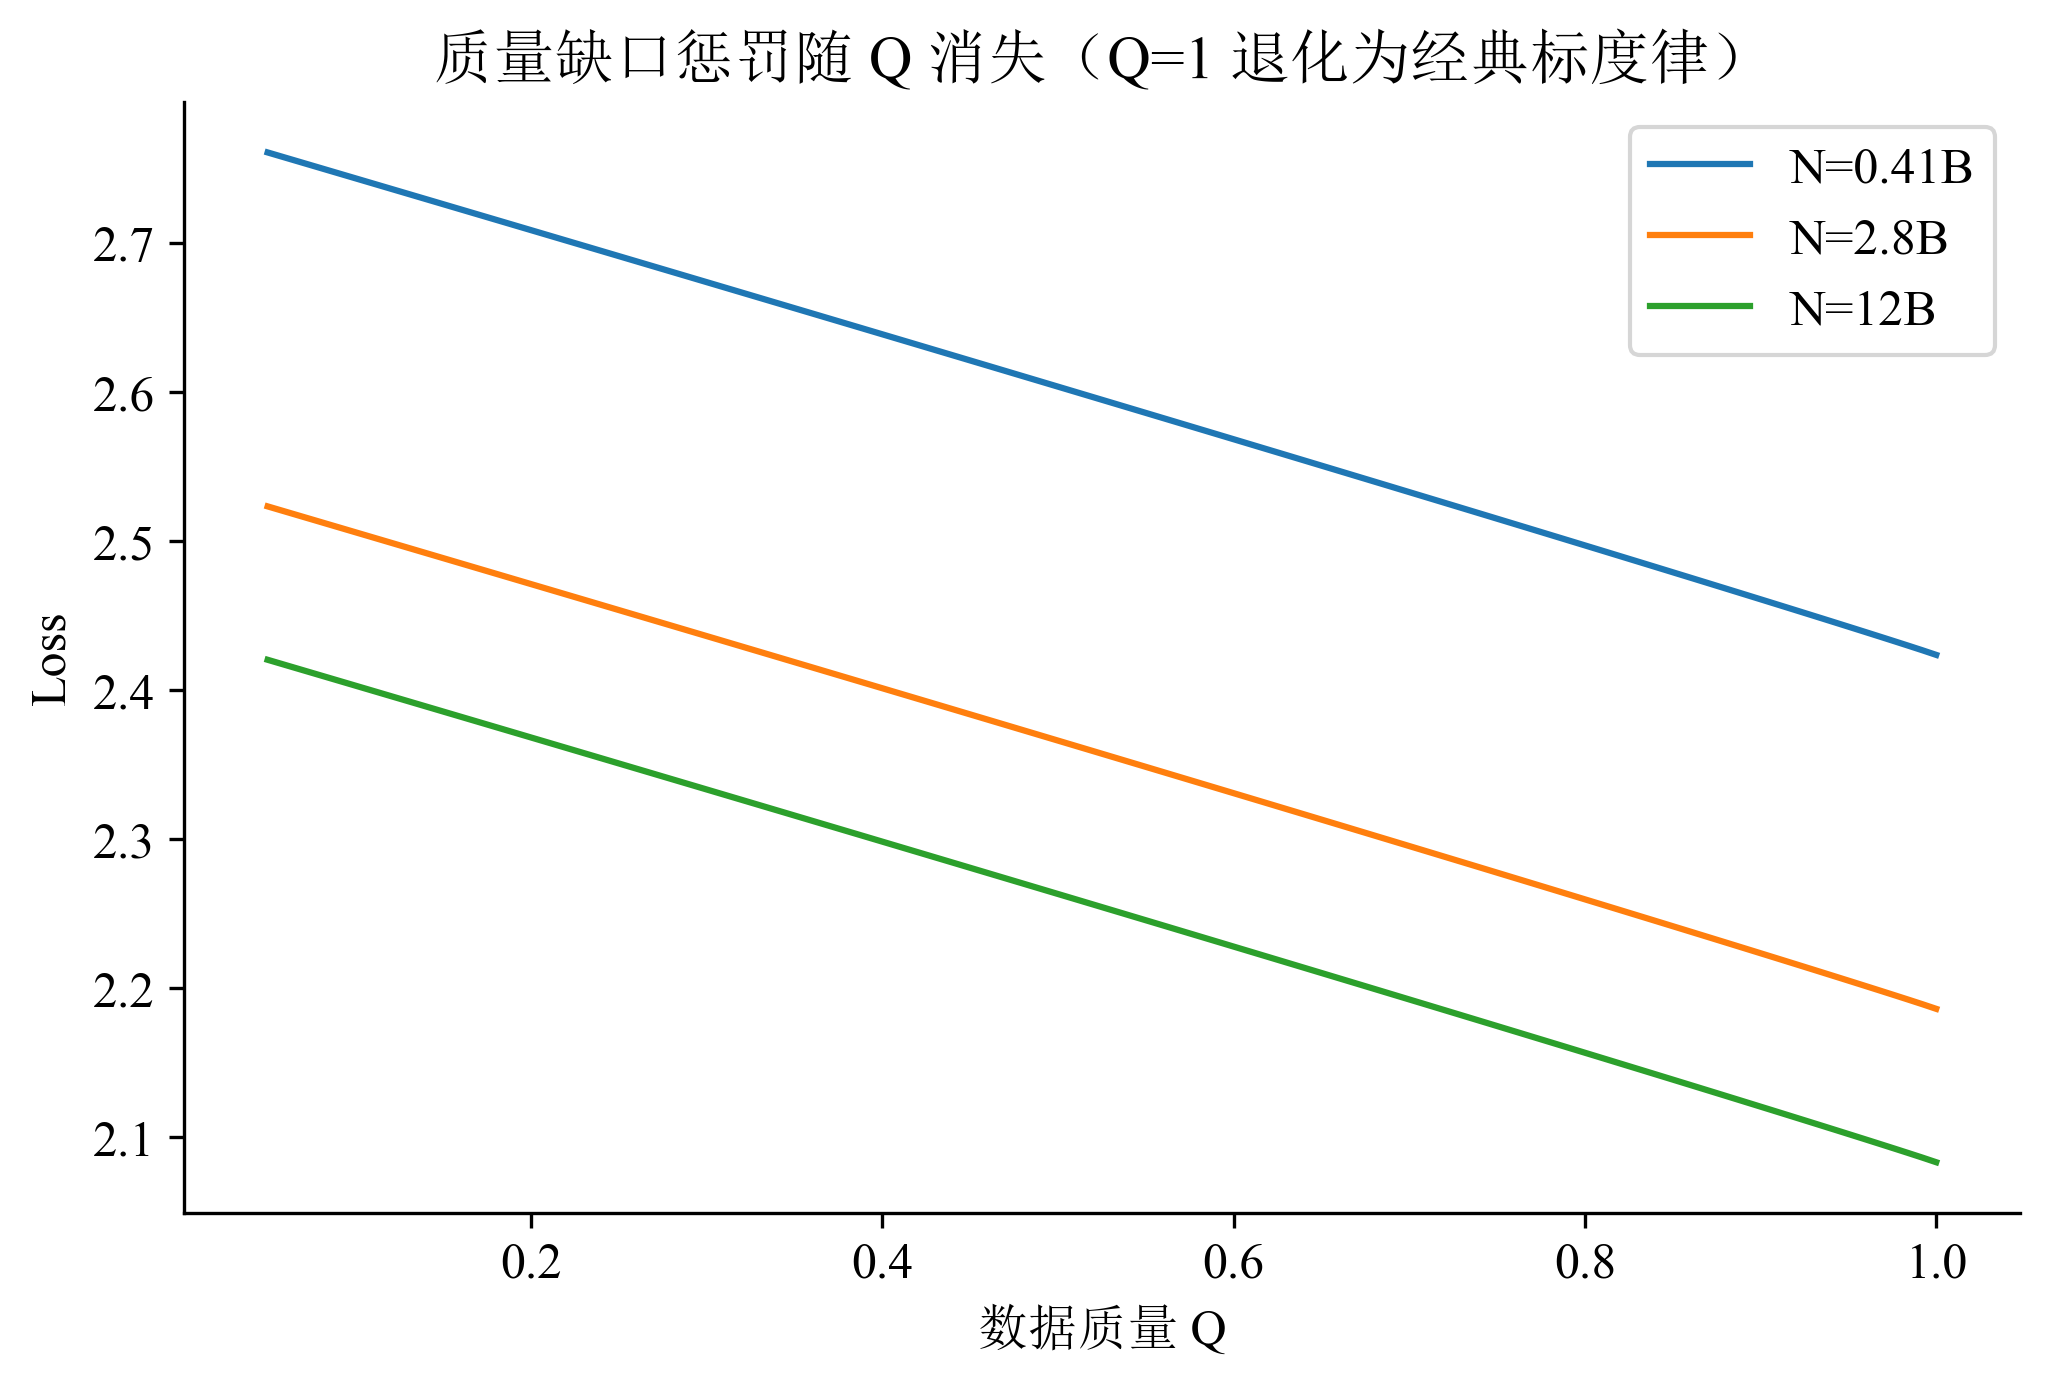
\includegraphics[width=0.62\textwidth]{求解/问题二/图片/图3_质量边际影响.png}
  \caption{固定 $N$、$D$ 时数据质量对损失的决定作用（$Q=1$ 退化为经典标度律）}
  \label{fig:p2_quality}
\end{figure}

\textbf{3.分层验证与稳健性}

广义标度律在 6 个独立来源上的分层验证结果如表\ref{tab:p2_val}所示，预测—实测对比如图\ref{fig:p2_general}所示。

\begin{longtable}{>{\raggedright\arraybackslash}p{0.32\textwidth}>{\centering\arraybackslash}p{0.10\textwidth}>{\centering\arraybackslash}p{0.14\textwidth}>{\centering\arraybackslash}p{0.12\textwidth}>{\centering\arraybackslash}p{0.12\textwidth}>{\centering\arraybackslash}p{0.12\textwidth}}
  \caption{广义标度律的分层验证}
  \label{tab:p2_val} \\
  \toprule
  验证来源 & 样本数 & 性质 & $r$ & RMSE & MAPE(\%) \\
  \midrule
  \endfirsthead
  \caption{广义标度律的分层验证（续）} \\
  \toprule
  验证来源 & 样本数 & 性质 & $r$ & RMSE & MAPE(\%) \\
  \midrule
  \endhead
  \bottomrule
  \endfoot
  B4 跨族收敛点 & 57 & 真实 & 0.975 & 0.293 & 8.8 \\
  B5 已发表标度律 & 44 & 真实 & 0.910 & 0.193 & 8.0 \\
  B7 质量扩展新增点 & 90 & 半合成 & 0.991 & 0.056 & 1.6 \\
  B10 百亿参数以上 & 128 & 估算 & 1.000 & 0.020 & 1.0 \\
  B2 Cerebras 族外 & 1{,}029 & 半合成 & 0.666 & 1.245 & 33.7 \\
  B8 大规模矩阵（方向重定向） & 984 & 半合成 & 0.638 & 1.294 & 133.4 \\
\end{longtable}

\begin{figure}[ht]
  \centering
  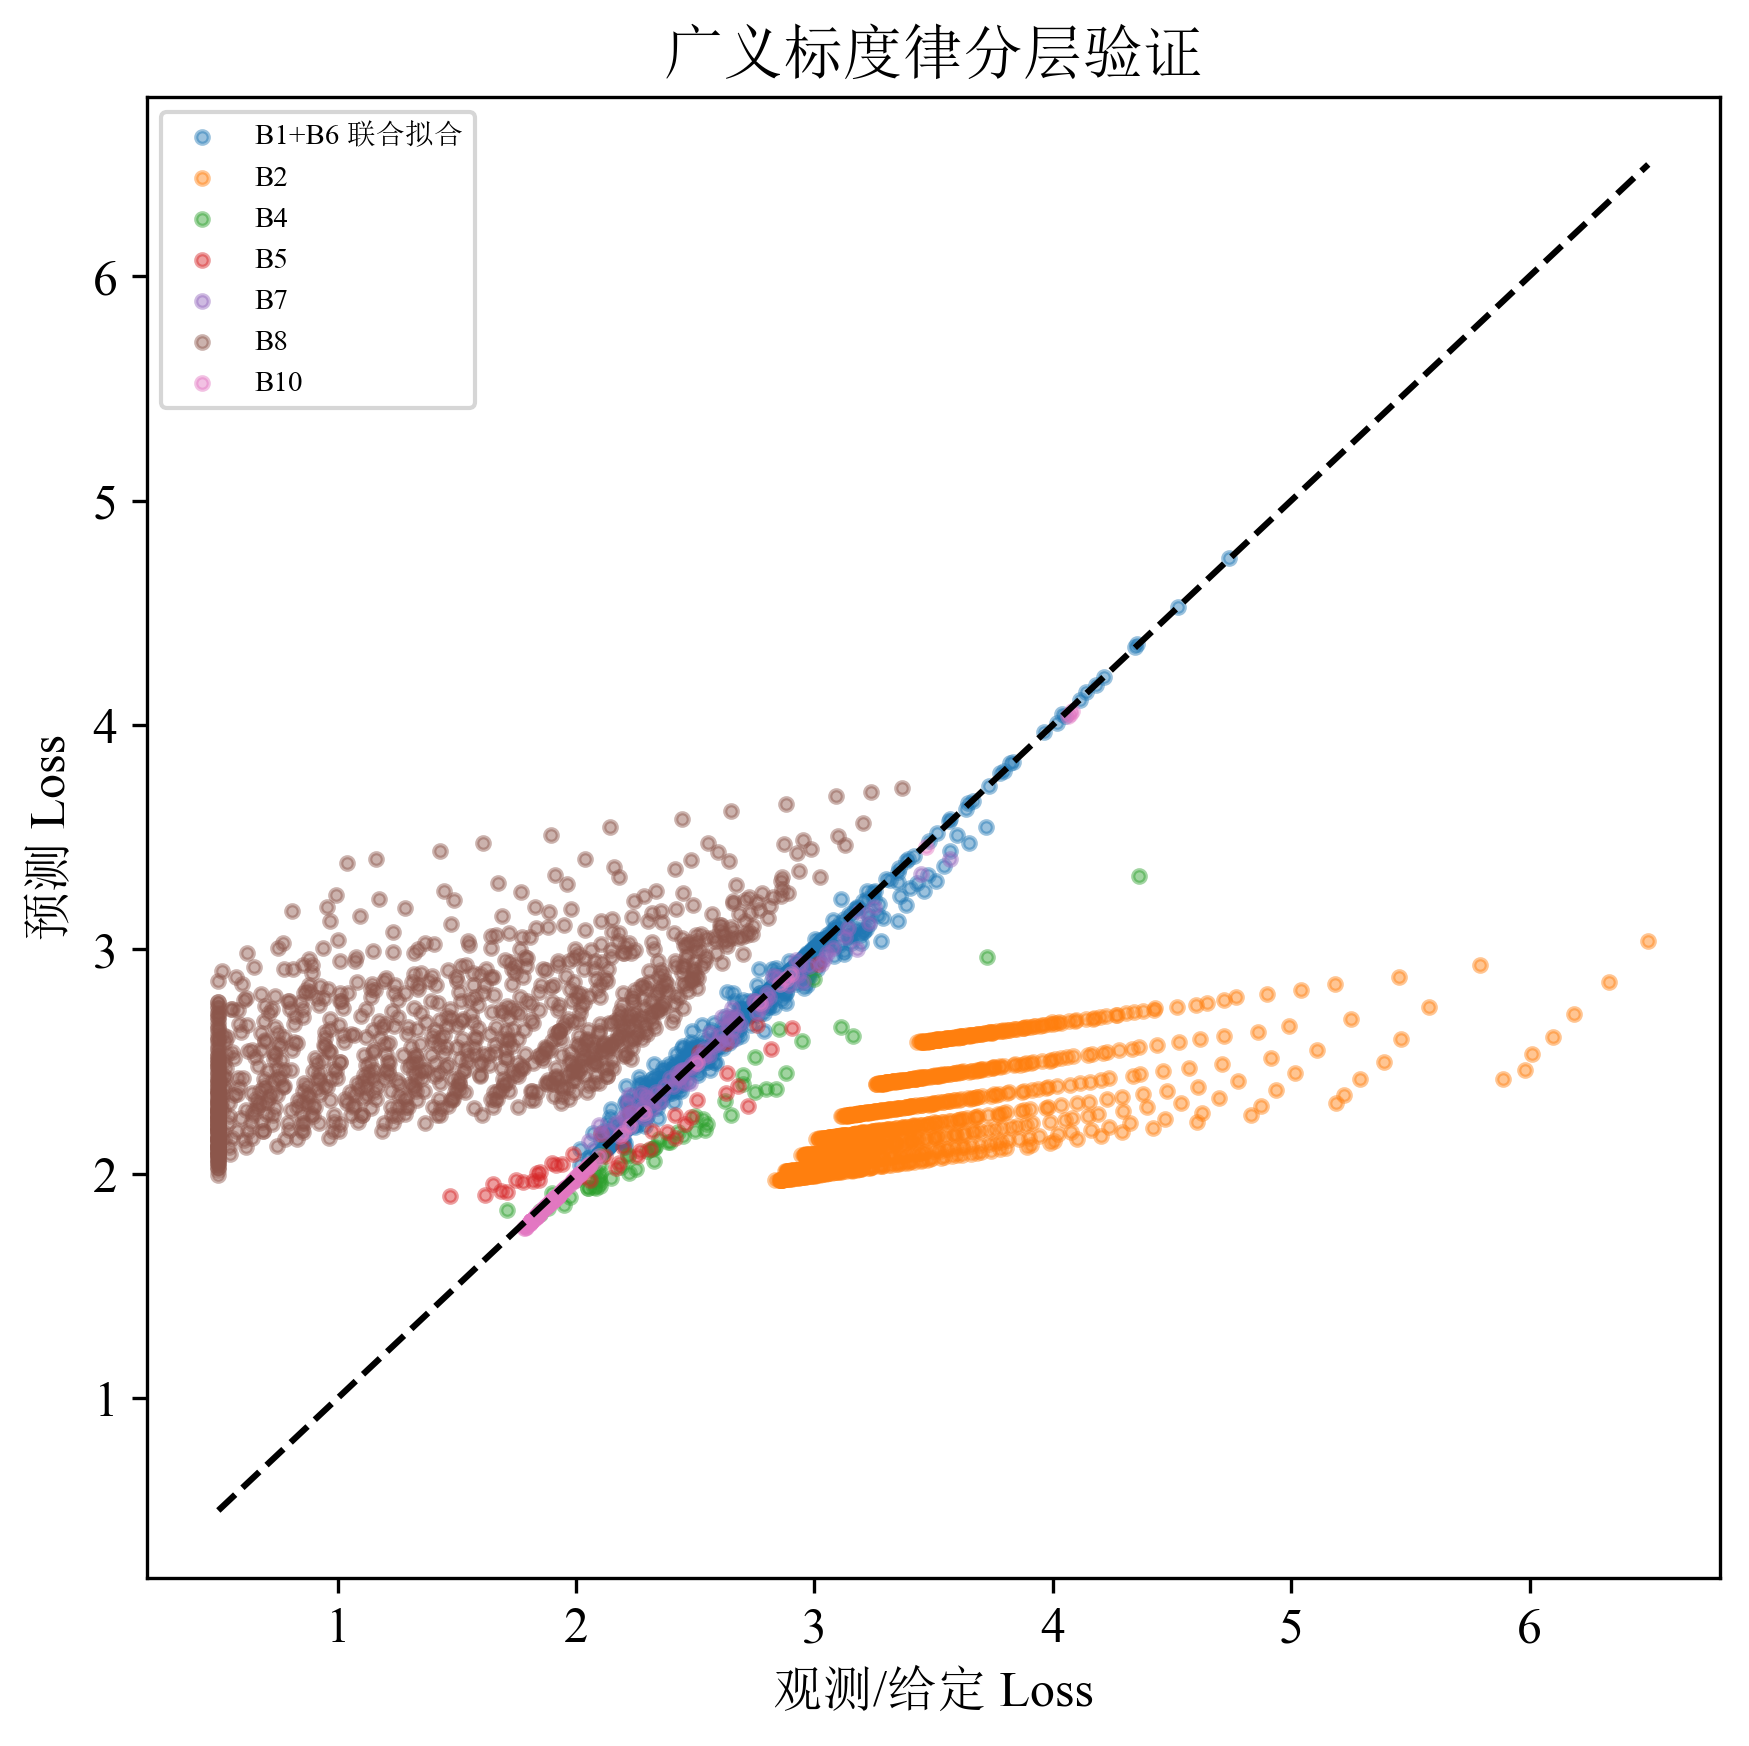
\includegraphics[width=0.62\textwidth]{求解/问题二/图片/图2_广义标度律验证.png}
  \caption{广义标度律预测值与实测损失的多源对比}
  \label{fig:p2_general}
\end{figure}

由表\ref{tab:p2_val}可知：（1）在真实数据上（B4 跨族、B5 文献），模型的相关达 $0.975$ 与 $0.910$、平均相对误差控制在 $8\%$ 量级，说明标度律具备跨族泛化能力；（2）在半合成质量数据上（B7 新增点、B10 估算），相关达 $0.991$ 与 $1.000$，验证了质量项的外推一致性；（3）B2（Cerebras 半合成轨迹）的 MAPE 达 $33.7\%$，说明该半合成数据的校准基线与 Pythia 标度律存在系统性差异，不宜作为定量验证依据；（4）B8 在大规模参数段的最小损失（$0.50$）低于模型不可约损失下限（$1.656$），即使按方向重定向后仍无法拟合（MAPE $133\%$），进一步印证其口径异常。上述分层结论明确界定了本文标度律的可信度边界：**定量结论适用于 $0.07\sim700$B 参数、$5\sim2\times10^4$B tokens 区间的真实与半合成（B6/B7）数据**；B2、B8 仅作定性参考。

此外，用 B3 的 8 条插值轨迹检验数据规模指数：在每条轨迹内（$N$ 固定）以 $L-(E+AN^{-\alpha})$ 对 $D$ 做双对数回归，得到的幂指数为 $-0.2806\sim-0.2803$，与经典拟合的 $-\beta=-0.2799$ 高度一致，说明数据标度关系在训练轨迹内部同样成立。

\textbf{4.弹性、替代关系与领域替代互补}

规模与质量的边际效用对比如图\ref{fig:p2_margin}所示，等损失曲线如图\ref{fig:p2_subst}所示，弹性与替代率计算结果如表\ref{tab:p2_subst}所示。

\begin{figure}[ht]
  \centering
  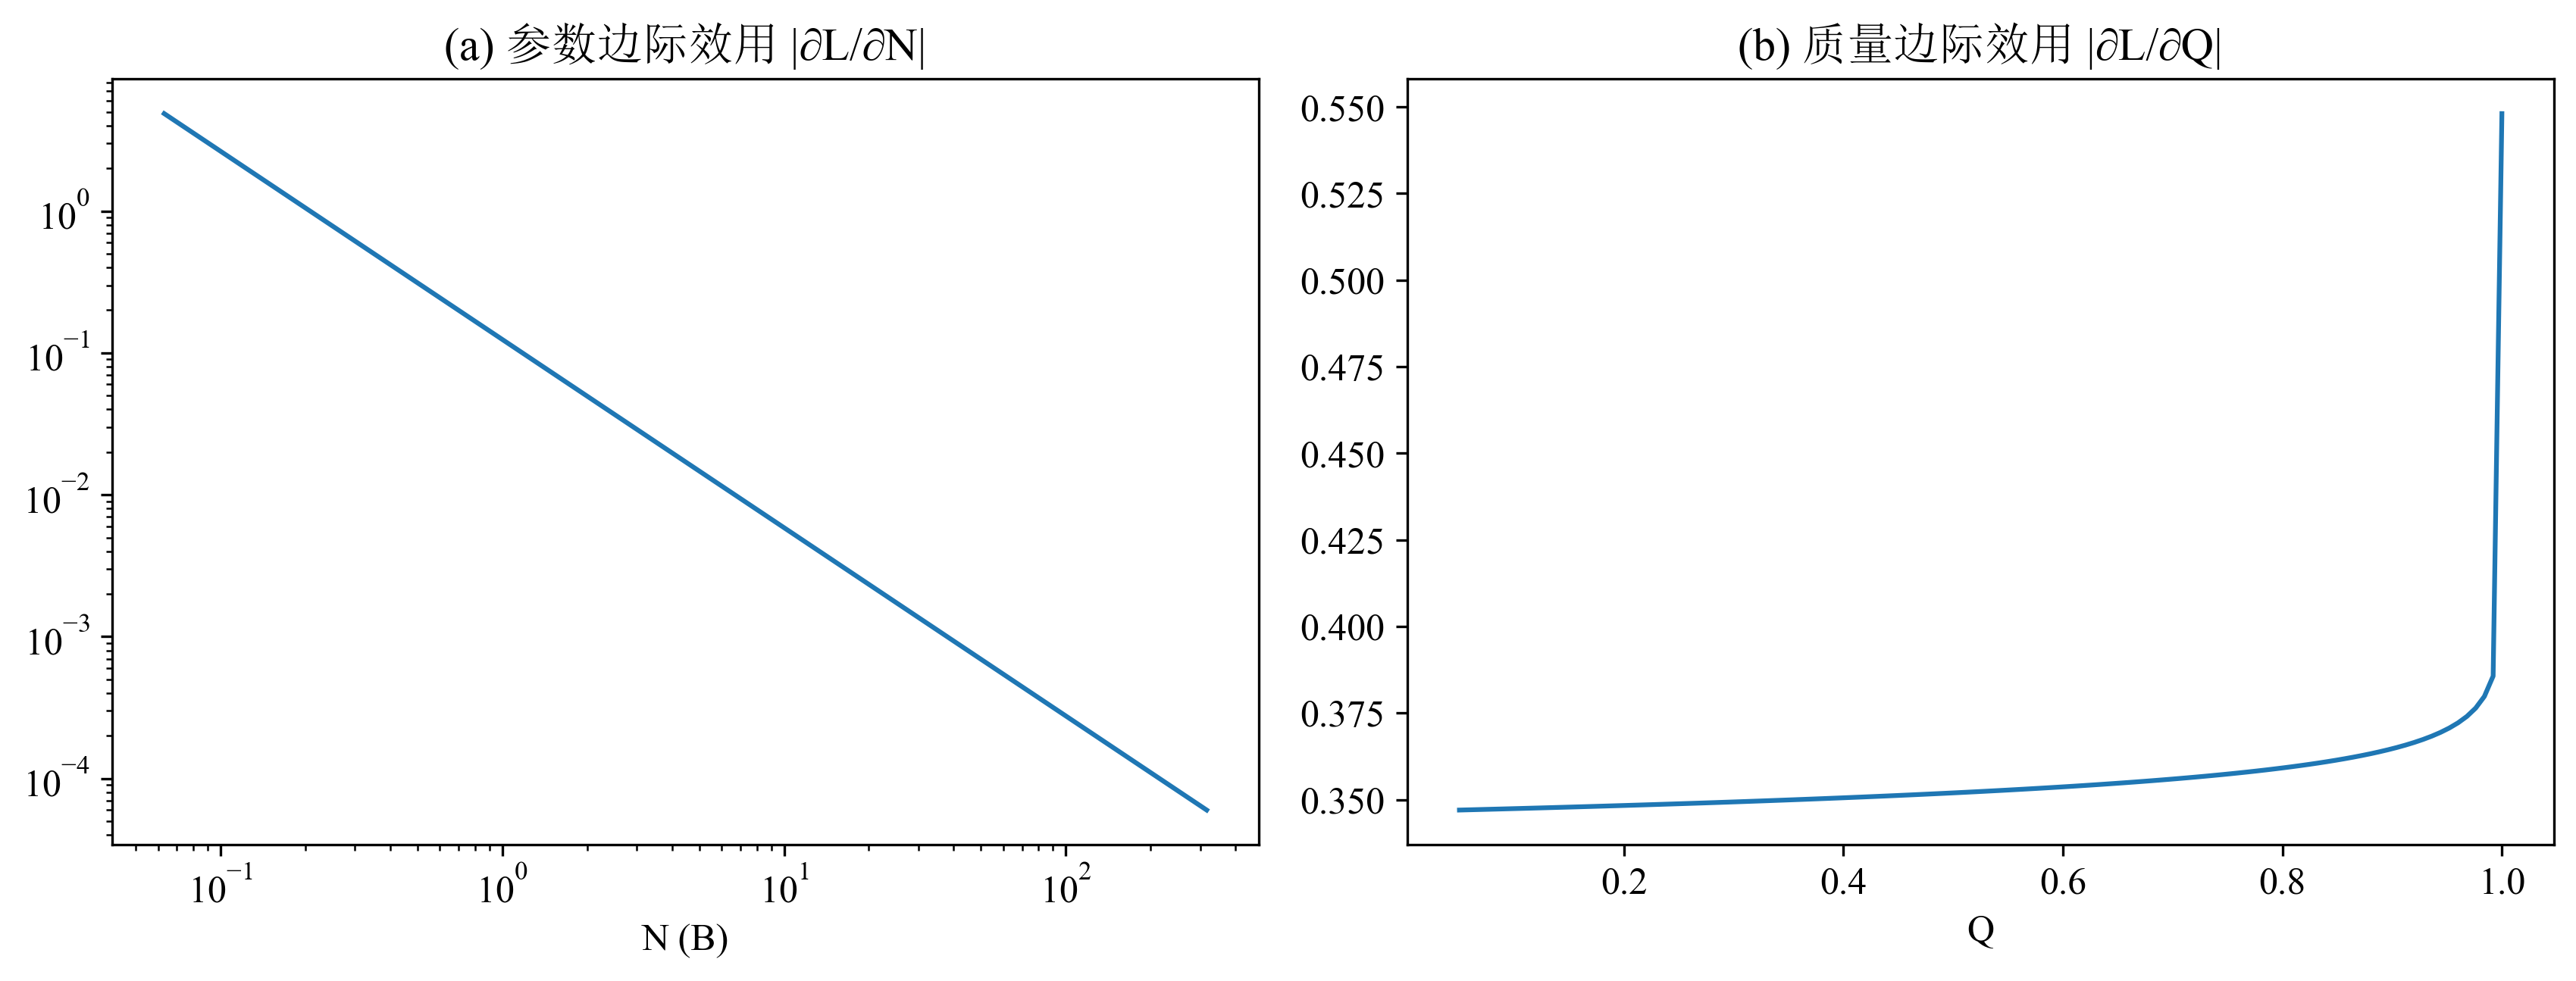
\includegraphics[width=0.92\textwidth]{求解/问题二/图片/图4_边际效用对比.png}
  \caption{规模边际效用与质量边际效用的对比（左：随 $N$ 衰减；右：随 $Q$ 递减）}
  \label{fig:p2_margin}
\end{figure}

\begin{figure}[ht]
  \centering
  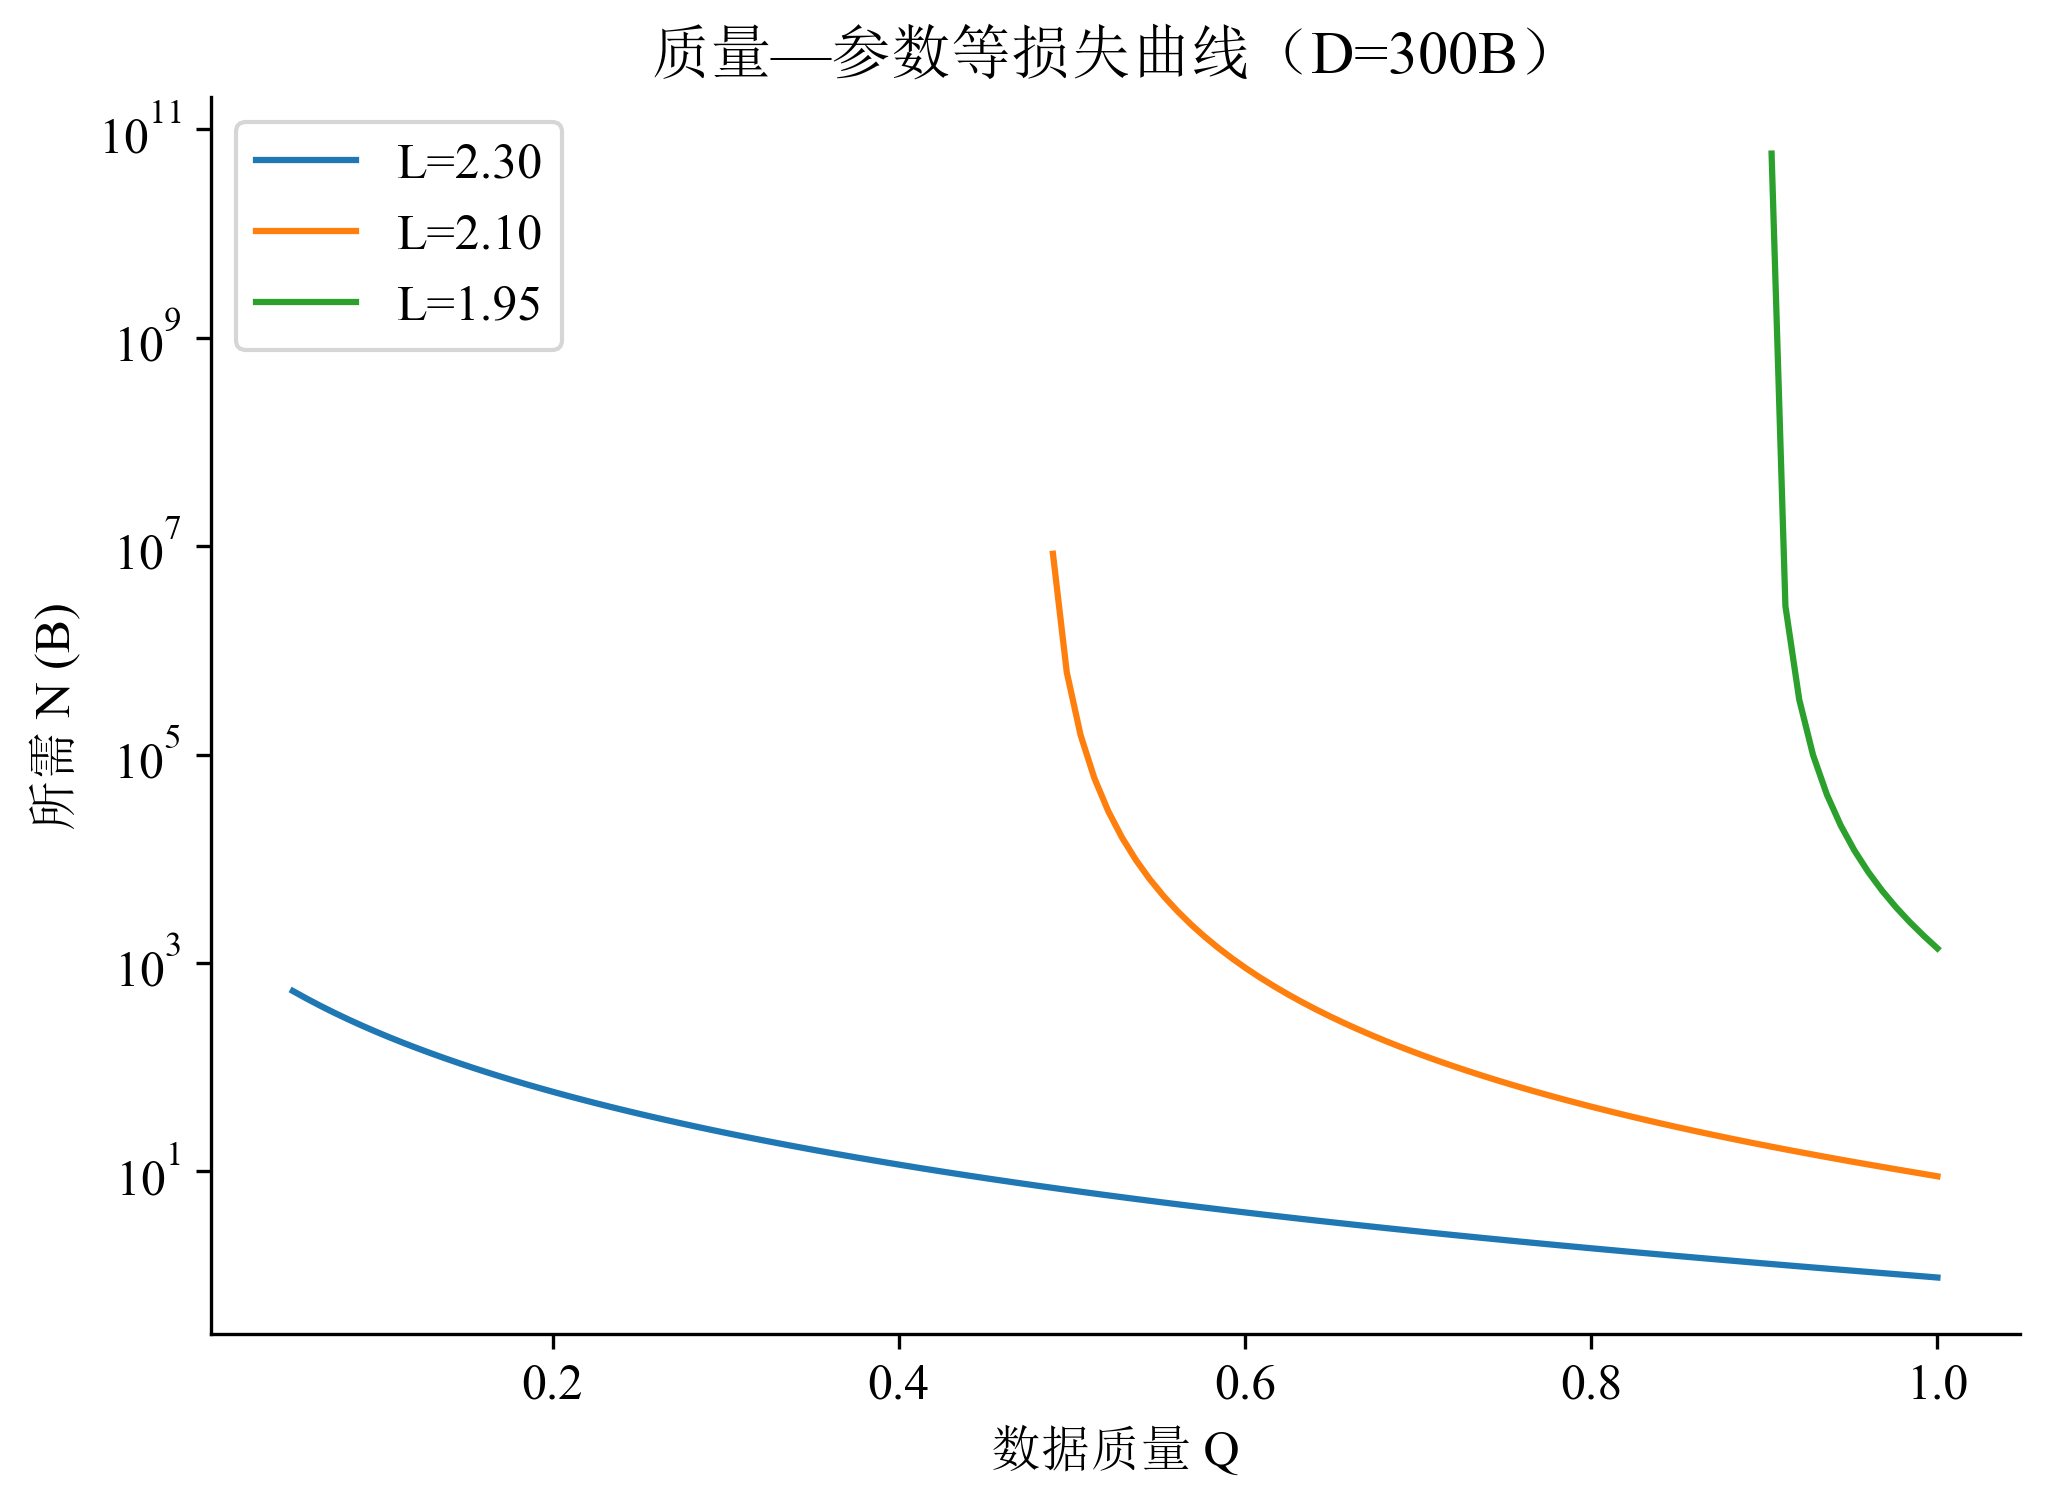
\includegraphics[width=0.60\textwidth]{求解/问题二/图片/图5_质量参数替代.png}
  \caption{等损失曲线：达到同一损失所需参数量随质量的演化（$D=300$B）}
  \label{fig:p2_subst}
\end{figure}

\begin{longtable}{>{\centering\arraybackslash}p{0.13\textwidth}>{\centering\arraybackslash}p{0.11\textwidth}>{\centering\arraybackslash}p{0.10\textwidth}>{\centering\arraybackslash}p{0.13\textwidth}>{\centering\arraybackslash}p{0.13\textwidth}>{\centering\arraybackslash}p{0.13\textwidth}>{\raggedright\arraybackslash}p{0.20\textwidth}}
  \caption{弹性与质量—参数替代关系}
  \label{tab:p2_subst} \\
  \toprule
  $N_0$(B) & $D_0$(B) & $Q_0$ & $\varepsilon_N$ & $\varepsilon_D$ & $\varepsilon_Q$ & $\mathrm dN/\mathrm dQ$ (B/单位) \\
  \midrule
  \endfirsthead
  \caption{弹性与质量—参数替代关系（续）} \\
  \toprule
  $N_0$(B) & $D_0$(B) & $Q_0$ & $\varepsilon_N$ & $\varepsilon_D$ & $\varepsilon_Q$ & $\mathrm dN/\mathrm dQ$ (B/单位) \\
  \midrule
  \endhead
  \bottomrule
  \endfoot
  1 & 100 & 0.6 & $-0.0491$ & $-0.0383$ & $-0.0838$ & 2.844 \\
  12 & 300 & 0.6 & $-0.0248$ & $-0.0321$ & $-0.0953$ & 76.838 \\
\end{longtable}

由表\ref{tab:p2_subst}可知：（1）在 $N_0=1$B、$D_0=100$B、$Q_0=0.6$ 处，质量弹性 $|\varepsilon_Q|=0.0838$ 约为规模弹性 $|\varepsilon_N|=0.0491$ 的 $1.7$ 倍，即在同等比例投入下质量提升对损失的压制更强；（2）替代率 $\mathrm dN/\mathrm dQ=2.844$ B/单位质量，即数据质量提升 $0.1$ 所带来的损失下降等价于参数量增加约 $0.28$B；（3）替代率随 $N$ 迅速增大（在 $N_0=12$B 处达 $76.8$ B/单位，$0.1$ 的质量提升等价于约 $7.68$B 参数），验证了式 $\mathrm dN/\mathrm dQ\propto N^{\alpha+1}$ 的结论——**规模越大，以质量换规模越划算**。图\ref{fig:p2_subst}的等损失曲线进一步显示，随着质量提高，达到同一损失所需参数量指数级下降。

领域间的替代与互补结构如图\ref{fig:p2_dom}所示。

\begin{figure}[ht]
  \centering
  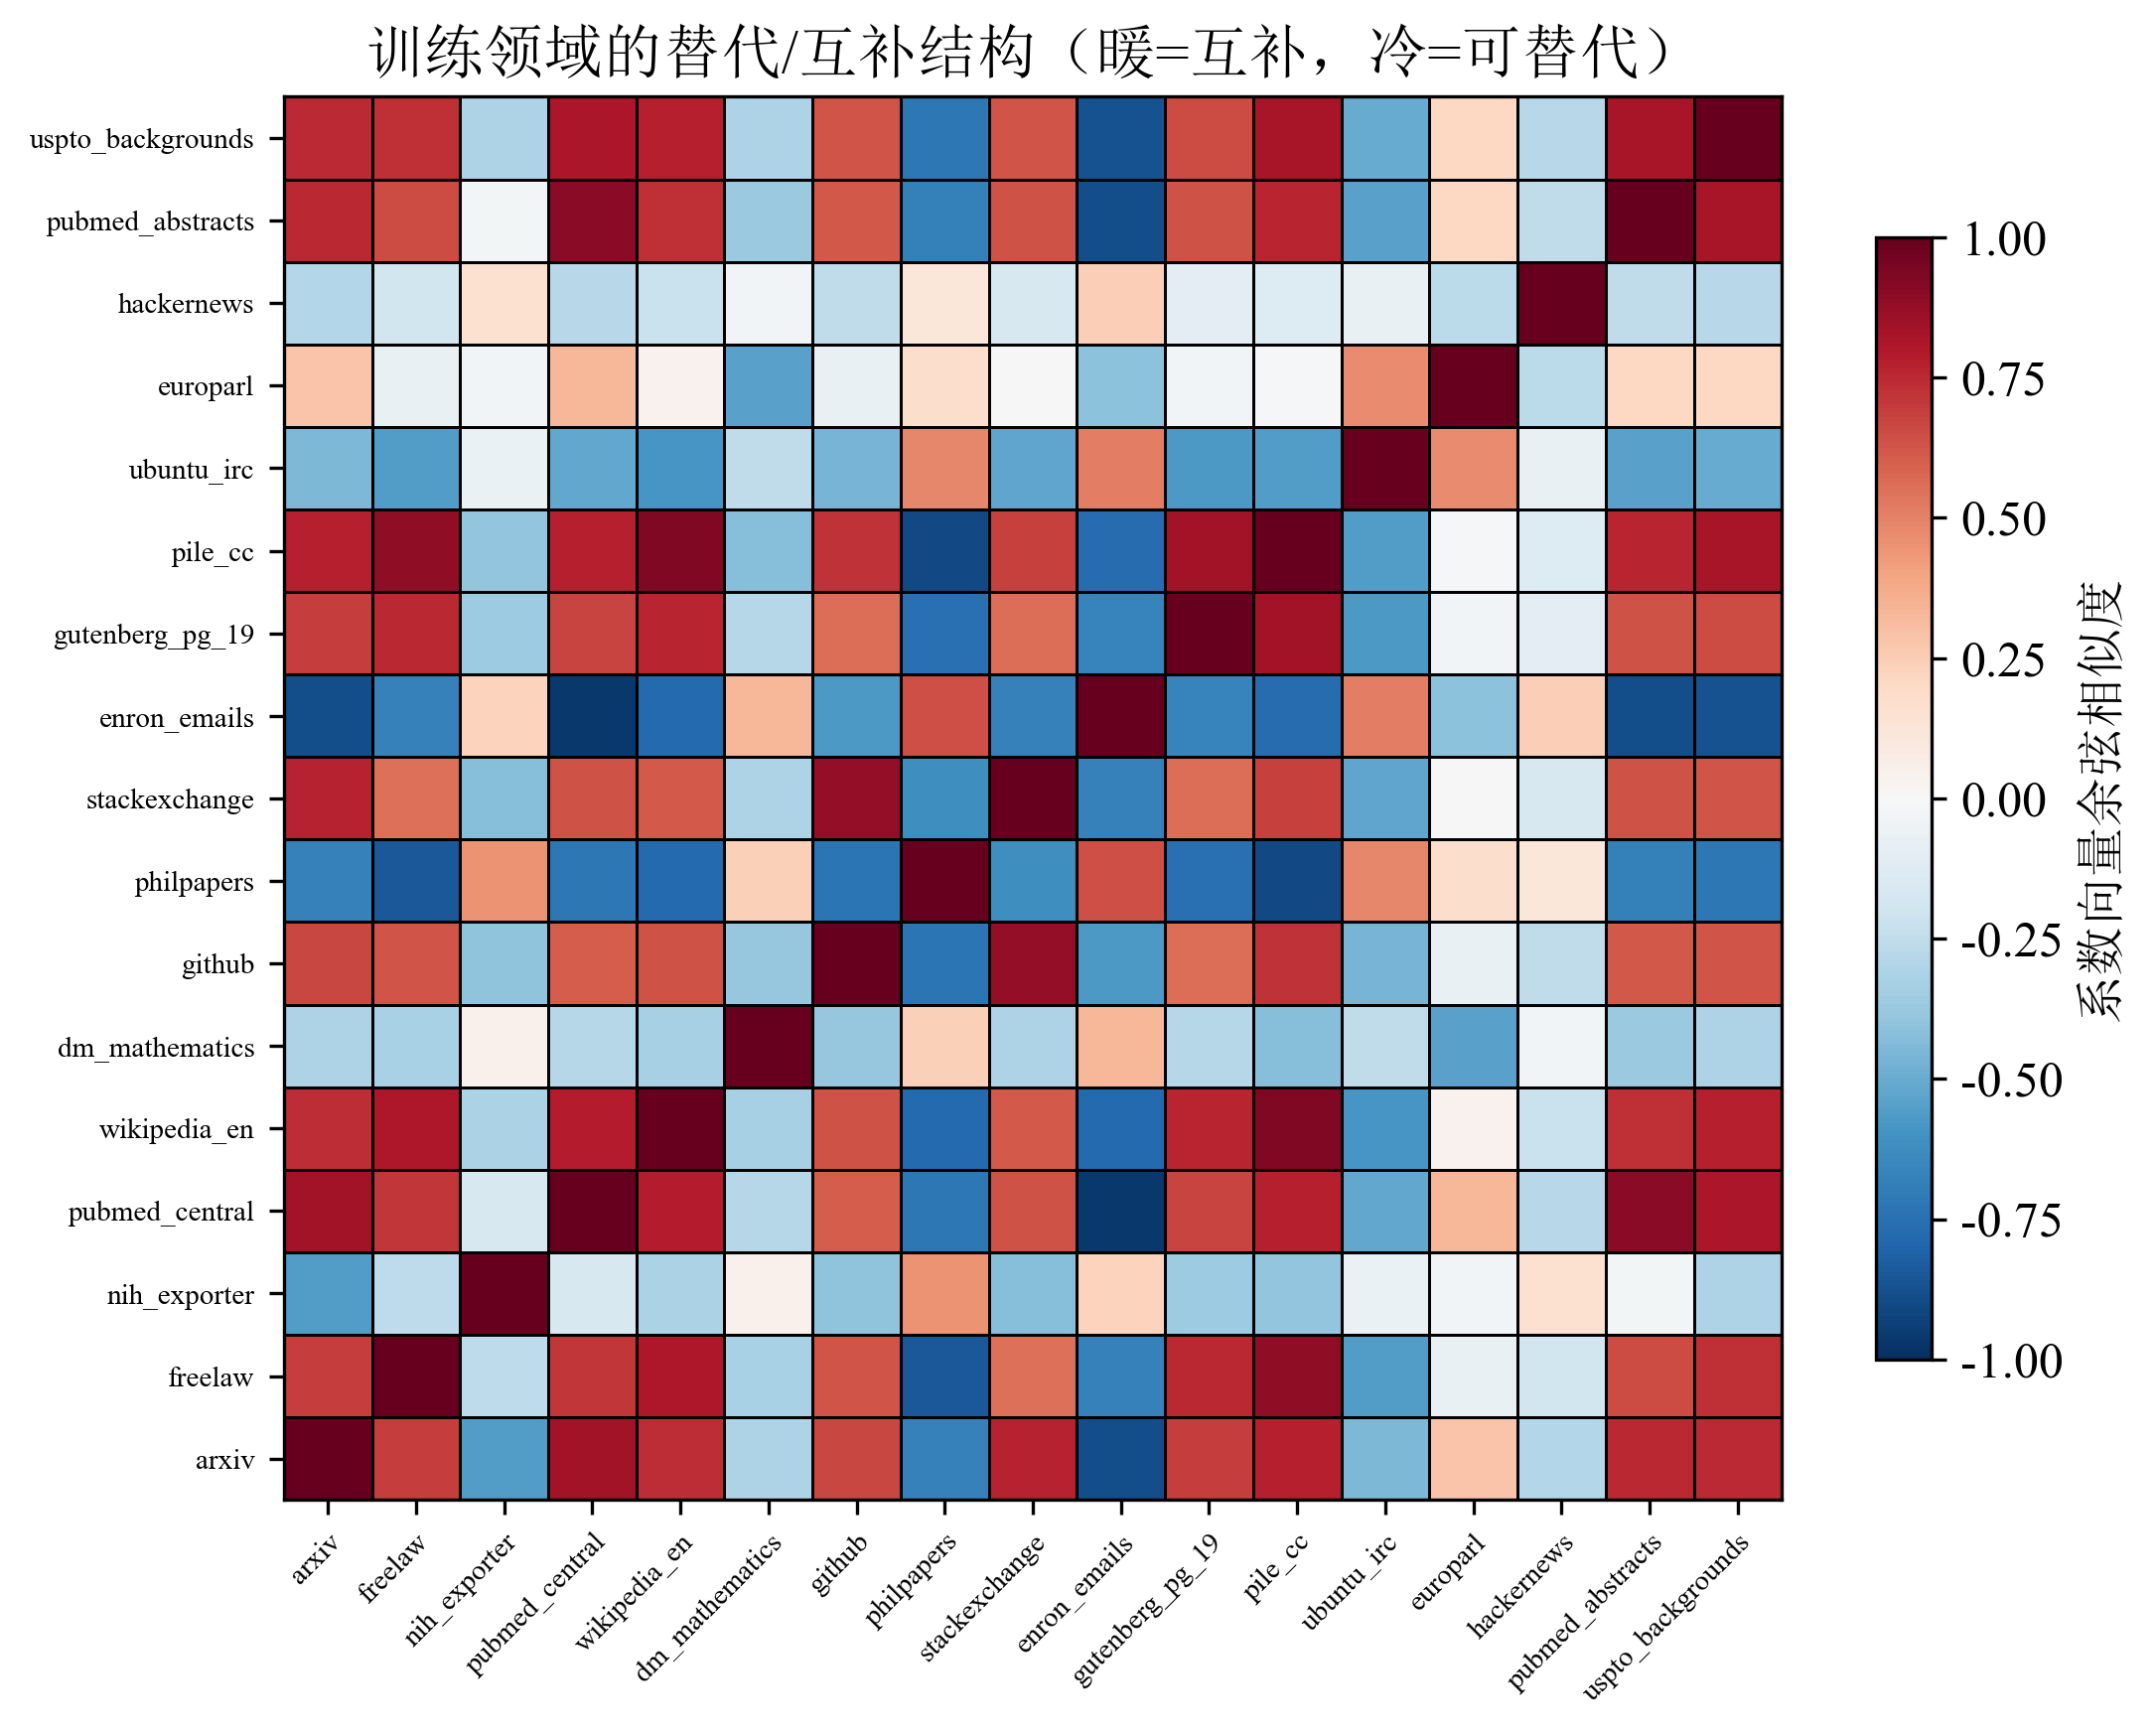
\includegraphics[width=0.62\textwidth]{求解/问题二/图片/图6_领域替代互补.png}
  \caption{训练领域的替代/互补结构（系数向量余弦相似度，暖=互补、冷=可替代）}
  \label{fig:p2_dom}
\end{figure}

由图\ref{fig:p2_dom}可知，（wikipedia\_en, pile\_cc）与（pubmed\_central, pubmed\_abstracts）的相似度最高（$0.925$、$0.903$），即它们对 13 个验证域的作用方式趋同，在配比中互为替代品；而（pubmed\_central, enron\_emails）的相似度为 $-0.967$、作用方式相反，构成互补对。这一结构解释了问题一推荐配比中“学术类域同时上升、网页类域同时下降”的成组变动现象：优化算法实际是在同一替代族内重新分配权重，而非逐域独立调整。

最后，将问题一的推荐配比作为配比项 $M(\bm p)$ 引入广义标度律（$M=\hat L(\bm p_{\text{rec}})-\hat L(\bm p_{\text{ref}})=-0.1988$，即在同等算力下损失下降 $0.199$），说明领域配比虽不增加算力总开销，却能改变算力的使用效率；该修正项将在问题三中作为损失函数的水平平移参与优化。

综合以上结果，本节完成了问题二的求解，得到广义标度律 $L(N,D,Q)$、质量与规模的替代条件以及领域替代互补结构，为问题三提供优化目标。

\subsection{问题三的模型的建立和求解}

\subsubsection{具体分析}

针对问题三，本问属于\textbf{约束优化与资源配置}类问题，需要在给定算力预算下联合优化参数量 $N$、数据量 $D$、领域配比 $\bm p$ 与数据质量 $Q$，并分析预算跨越不同量级时资源配置是否发生结构性转移。本问综合采用“损失函数 $+$ 成本函数 $+$ 约束优化”的框架：以问题二导出的广义标度律 $L(N,D,Q)$ 为优化目标；严格按赛题给出的三部分公式建立总成本模型——基础训练 $6ND$、质量提升 $D[g(Q)-g(Q_0)]_+$、长文本注意力 $\eta N D L_{\text{ctx}}$；在总成本不超过预算的约束下用序列二次规划（SLSQP）在对数尺度上求解最优 $(N,D,Q)$；最后通过预算扫略与临界上下文长度分析识别结构性转移。

首先由问题二输出的广义标度律参数与问题一输出的质量基线 $Q_0$ 构建优化目标与约束；其次解析给出使注意力开销与训练开销相等的临界上下文长度 $L_{\text{crit}}=6/\eta$，并以附件 C7 的最大上下文长度字段确定 $L_{\text{ctx}}$ 的可行取值；然后在低、中、高三档预算下联合优化 $N$、$D$、$Q$，并对比附录 B 规定的三种质量成本函数；最后扫描 $10^{18}$–$10^{25}$ FLOPs 的连续预算，定量刻画最优质量与预算份额的结构性转移。

\subsubsection{模型准备}

\textbf{1.数据预处理}

本问的标度律参数直接读取问题二的输出 $\{E,A,\alpha,B,\beta,C,\gamma\}=\{1.6558,0.3808,0.3266,1.2515,0.2767,0.3544,0.9779\}$，保证两问模型一致。

基线质量 $Q_0$ 由附件 A 的质量评分给出。考虑到 A1--A3 的抽样设计使 github 域占比偏高，直接取全量样本均值会低估真实语料的平均质量，故本文以**参考语料配比加权**的方式定义基线：
\begin{equation}
    Q_0 = \sum_{k=1}^{17} \bar p_k\, Q_k = 0.5510
\end{equation}
其中 $\bar p_k$ 为 A4 训练配方的平均配比，$Q_k$ 为该配方域经 A16 映射得到的质量评分。作为对照，全量样本的未加权质量均值为 $0.4952$（该口径在误差分析中作为灵敏度检验项）。

上下文长度 $L_{\text{ctx}}$ 由模型架构与任务需求外生给定，其可行取值依据附件 C7 的 max\_position\_embeddings 字段，为 $\{2048,\ 4096,\ 8192,\ 32768,\ 131072\}$ 五个档位；本问不将其作为内点寻优变量，仅考察其取值对最优配置的影响。

质量可行域由数据支持范围确定：B6/B7 覆盖 $Q_{\text{score}}\in[0.10,1.00]$，且当 $Q=1$ 时广义标度律精确退化为经典形式（损失为 $E+A/N^{\alpha}+B/D^{\beta}>0$，不产生非物理负值），故可行域取 $Q\in[Q_0,1]$，下限为基线质量（质量不提升时质量成本为零）。

\textbf{2.算法选择}

本问核心是带非线性约束的连续优化，候选方法包括序列二次规划（SLSQP）、内点法与遗传算法。本问题目标与约束均为光滑函数，SLSQP 能高效处理预算不等式约束与变量界约束，且通过对数变换参数化 $N$、$D$（以 $\ln N$、$\ln D$ 为变量）可消除尺度病态、改善收敛；为避免局部最优，本文以 8 组不同初值分别求解并取最优解。遗传算法虽具全局搜索能力，但收敛慢、精度低，不适合本问题对精度的要求。

\subsubsection{模型建立}

\textbf{步骤1：优化目标}

以问题二的广义标度律为优化目标，并计入问题一给出的配比项平移 $M(\bm p)$：
\begin{equation}
    \min_{N,D,Q}\ L(N,D,Q) = E + \frac{A}{N^{\alpha}} + \frac{B}{D^{\beta}} + C\,(1-Q)^{\gamma} + M(\bm p)
\end{equation}
其中 $M(\bm p)=\hat L(\bm p)-\hat L(\bm p_{\text{ref}})$ 由问题一的线性混合回归给出，刻画领域配比的效率增益（不消耗额外算力）。本文按“由前两问结果确定”的方式处理 $\bm p$：取问题一的有界推荐配比，对应 $M=-0.1988$；在求解中同时报告参考配比（$M=0$）的结果以作对照，理由见步骤 5。

\textbf{步骤2：总成本模型}

总算力成本由基础训练、质量提升与长文本注意力三部分构成：
\begin{equation}
    C(N,D,Q;L_{\text{ctx}}) = \underbrace{6ND}_{C_{\text{train}}}
    + \underbrace{D\left[g(Q)-g(Q_0)\right]_{+}}_{C_Q}
    + \underbrace{\eta\,N\,D\,L_{\text{ctx}}}_{C_{\text{attn}}},
    \qquad \eta = 2\times10^{-4}
\end{equation}
其中基础训练采用 Chinchilla 近似 $C_{\text{train}}\approx 6ND$；质量提升项中的 $[\cdot]_+=\max(\cdot,0)$ 表示质量只提升不降低；质量成本函数 $g(Q)$ 从附录 B 规定的三型中选取：
\begin{equation}
    g_{\text{指数}}(Q)=10^{7}e^{6.0Q},\qquad
    g_{\text{幂函数}}(Q)=5\times10^{9}Q^{4.0},\qquad
    g_{\text{对数渐进}}(Q)=2\times10^{9}\ln(1+10.0Q)
\end{equation}
注意 $C_Q$ 与训练 token 数 $D$ 成正比，即“质量提升”是对全语料的处理开销，数据量越大、达到同样质量的总成本越高；这一结构与“质量成本与数据规模无关”的简化假设有本质区别，本文严格采用赛题给定形式。

\textbf{步骤3：临界上下文长度（解析解）}

由 $C_{\text{attn}}=C_{\text{train}}$ 即 $\eta N D L_{\text{ctx}}=6ND$，两端约去 $ND$ 得临界上下文长度：
\begin{equation}
    L_{\text{crit}} = \frac{6}{\eta} = \frac{6}{2\times10^{-4}} = 30{,}000\ \text{tokens}
\end{equation}
当 $L_{\text{ctx}}<L_{\text{crit}}$ 时基础训练仍是算力主体；当 $L_{\text{ctx}}>L_{\text{crit}}$ 时注意力开销超过基础训练、成为预算的主要消耗项。等价地，可定义“注意力开销倍数”$\lambda(L_{\text{ctx}})=\eta L_{\text{ctx}}/6=L_{\text{ctx}}/L_{\text{crit}}$，则总成本可重写为
\begin{equation}
    C=\left[1+\lambda(L_{\text{ctx}})\right]\cdot 6ND + D\left[g(Q)-g(Q_0)\right]_{+}
\end{equation}
即**长上下文把基础训练的单价放大了 $1+\lambda$ 倍**，这是后续结构性分析与敏感性分析的解析基础。

\textbf{步骤4：约束优化模型与最优性条件}

综合目标与成本，得到约束优化问题：
\begin{equation}
    \min_{\ln N,\ln D,Q}\ L(e^{\ln N},e^{\ln D},Q)
    \quad\text{s.t.}\quad
    C(N,D,Q;L_{\text{ctx}})\le C_{\text{budget}},\qquad Q\in[Q_0,1]
\end{equation}
为解释数值结果，对固定 $Q$ 的内点解可给出解析最优性条件。记 $K_1=6[1+\lambda(L_{\text{ctx}})]$、$K_2=g(Q)-g(Q_0)$，构造拉格朗日函数 $\mathcal L=A N^{-\alpha}+B D^{-\beta}+\mu(K_1ND+K_2D-C)$，由一阶条件消去 $\mu$ 得
\begin{equation}
    \alpha A N^{-\alpha-1}\left(N+\tau(Q)\right)=\beta B D^{-\beta},
    \qquad \tau(Q)\equiv\frac{K_2}{K_1}=\frac{g(Q)-g(Q_0)}{6\left[1+\lambda(L_{\text{ctx}})\right]}
    \label{eq:p3_balance}
\end{equation}
其中 $\tau(Q)$ 的量纲为 token，物理含义是**质量提升所对应的“等效附加数据量”**：把质量投入折算成必须额外处理的 token 数。当不投入质量（$Q=Q_0$，$\tau=0$）时式\eqref{eq:p3_balance}退化为经典平衡条件 $\alpha A N^{-\alpha}=\beta B D^{-\beta}$，可得
\begin{equation}
    D \propto N^{\alpha/\beta},\qquad
    N^{*}\propto C^{\frac{\beta}{\alpha+\beta}},\qquad
    D^{*}\propto C^{\frac{\alpha}{\alpha+\beta}}
\end{equation}
由于 $\alpha>\beta$，数据量随预算增长的速度快于参数量，$D/N$ 比随预算上升。而 $\tau(Q)>0$ 相当于在参数量上追加了一笔“质量附加成本”，会同时抑制 $N$ 与 $D$，并使最优 $Q$ 与预算之间的取舍关系呈现非线性。

\textbf{步骤5：结构性转移的定义与识别方法}

“结构性转移”指最优策略发生质变而非量的连续变化。本文给出两级可操作定义：
\begin{itemize}[itemindent=2em]
\item \textbf{拐点型转移：} 令 $f_{\text{qual}}(C)$ 为质量投入在总预算中的份额，$Q^{*}(C)$ 为最优质量。定义质量提升完成度 $\Theta(C)=\dfrac{Q^{*}(C)-Q_0}{1-Q_0}\in[0,1]$ 及其弹性 $e_\Theta=\dfrac{\mathrm d\ln\Theta}{\mathrm d\ln C}$。当 $e_\Theta$ 取得极大值、且 $\mathrm d f_{\text{qual}}/\mathrm d\ln C$ 由正转负时，表明预算的边际增量从“继续提升质量”转向“扩张规模”，构成一次结构性转移。
\item \textbf{角点型转移：} 当 $Q^{*}(C)$ 由上界约束 $Q=1$ 决定（而非内点最优）时，质量不再是可调节的边际资源，模型进入“质量饱和”制度；使 $Q^{*}$ 首次达到给定水平 $\bar Q$ 的预算 $C^{*}(\bar Q)$ 即为该制度的进入门槛，可由预算扫略直接读出。
\end{itemize}
本文在 $[10^{18},10^{25}]$ FLOPs 上以对数等距取 141 个预算点求解，报告上述两类门槛，并以 $C^{*}(0.5)$、$C^{*}(0.9)$、$C^{*}(0.99)$ 作为制度切换的标志点。

\subsubsection{模型求解}

\textbf{1.三种质量成本函数下的三档预算最优配置}

三档预算（$10^{19}$、$10^{22}$、$10^{24}$ FLOPs，覆盖低、中、高三个数量级）在幂函数型质量成本与 $L_{\text{ctx}}=2048$ 下的最优配置如表\ref{tab:p3_opt}所示，并以图\ref{fig:p3_opt}给出直观对比。

\begin{figure}[ht]
  \centering
  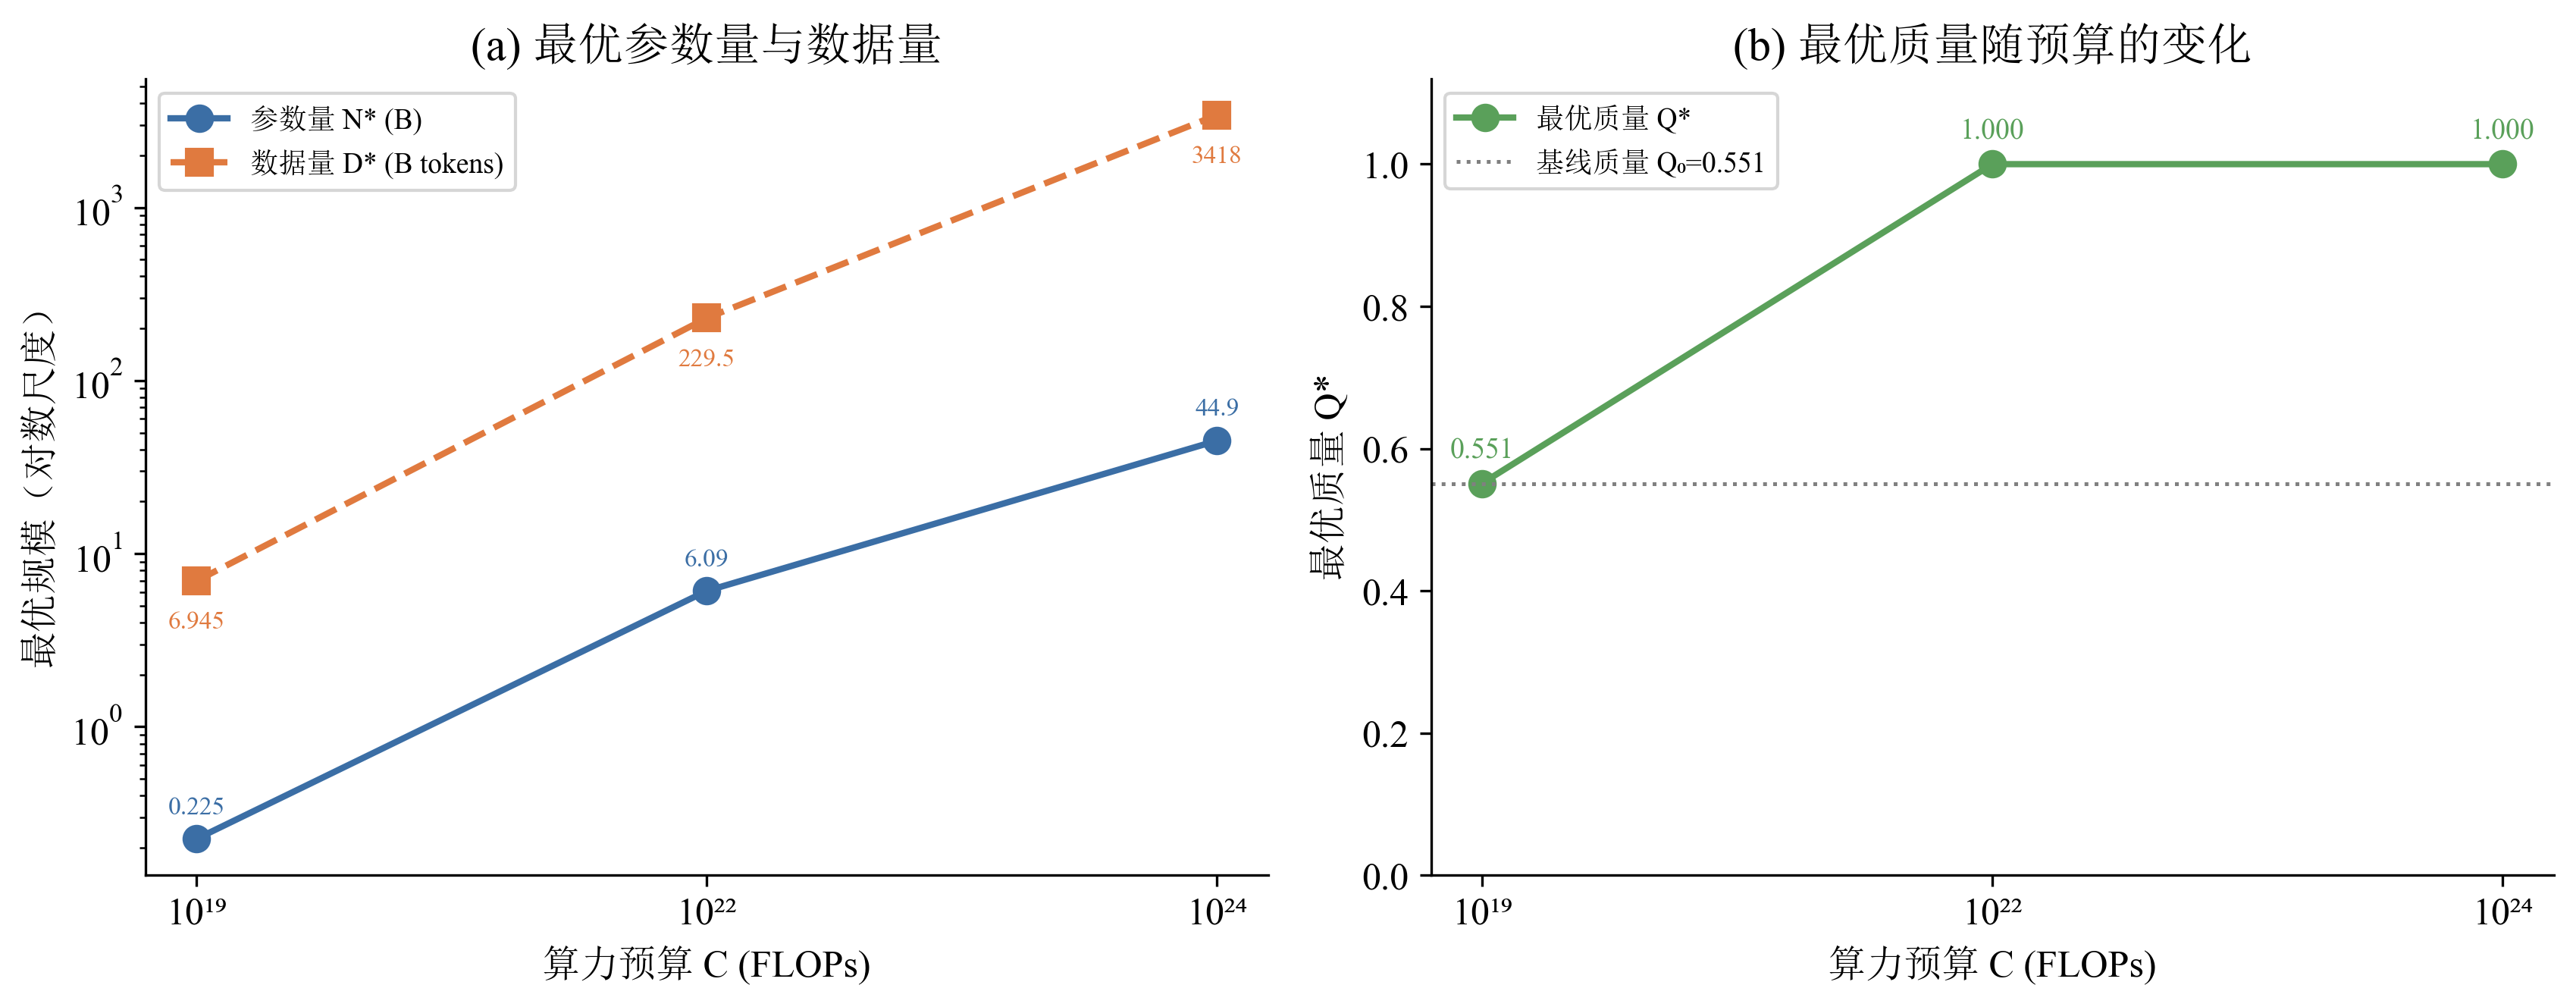
\includegraphics[width=0.72\textwidth]{求解/问题三/图片/图1_三档预算最优配置.png}
  \caption{三档算力预算下的最优资源配置（$N^*$、$D^*$、$Q^*$）}
  \label{fig:p3_opt}
\end{figure}

\begin{longtable}{>{\centering\arraybackslash}p{0.13\textwidth}>{\centering\arraybackslash}p{0.13\textwidth}>{\centering\arraybackslash}p{0.14\textwidth}>{\centering\arraybackslash}p{0.11\textwidth}>{\centering\arraybackslash}p{0.11\textwidth}>{\centering\arraybackslash}p{0.11\textwidth}>{\raggedright\arraybackslash}p{0.19\textwidth}}
  \caption{三档预算最优配置（幂函数型质量成本，$L_{\text{ctx}}=2048$）}
  \label{tab:p3_opt} \\
  \toprule
  预算 $C$ (FLOPs) & $N^{*}$ (B) & $D^{*}$ (B) & $Q^{*}$ & $L^{*}$ & $D^*/N^*$ & 预算份额（训练/质量/注意力） \\
  \midrule
  \endfirsthead
  \caption{三档预算最优配置（续）} \\
  \toprule
  预算 $C$ (FLOPs) & $N^{*}$ (B) & $D^{*}$ (B) & $Q^{*}$ & $L^{*}$ & $D^*/N^*$ & 预算份额 \\
  \midrule
  \endhead
  \bottomrule
  \endfoot
  $10^{19}$ & 0.225 & 6.9 & 0.551 & 3.170 & 30.9 & 93.6\% / 0.0\% / 6.4\% \\
  $10^{22}$ & 6.089 & 229.5 & 1.000 & 2.145 & 37.7 & 83.9\% / 10.4\% / 5.7\% \\
  $10^{24}$ & 44.937 & 3418.0 & 1.000 & 1.897 & 76.1 & 92.2\% / 1.6\% / 6.3\% \\
\end{longtable}

由表\ref{tab:p3_opt}可知：（1）随预算从 $10^{19}$ 升至 $10^{24}$ FLOPs，最优参数量由 $0.225$B 增至 $44.9$B、最优数据量由 $6.9$B 增至 $3418.0$B，验证了式 $N^{*}\propto C^{\beta/(\alpha+\beta)}$、$D^{*}\propto C^{\alpha/(\alpha+\beta)}$ 的解析结论；（2）$D/N$ 比由 $30.9$ 升至 $76.1$，与 $\alpha>\beta$ 的理论预期一致——由于参数规模的边际收益衰减更快，预算扩张更多流向数据；（3）最优质量由 $0.551$ 升至上界 $1.000$，中、高预算档均为“质量饱和”的角点解，说明**预算充裕时质量投入从“可选项”变为“必选动作”**；（4）低预算档（$10^{19}$）的最优质量恰好等于基线 $Q_0$、质量投入份额为 $0$——即在算力紧张时**完全不投资质量、把全部预算投向规模**，这比“质量投入比例较小”是更强的结论；高预算档质量份额降至 $1.6\%$ 并非因为质量不重要，而是因为 $Q$ 已触及上界、无需再投入。

三种质量成本函数（附录 B）下的最优配置对比如表\ref{tab:p3_cost}所示。

\begin{longtable}{>{\centering\arraybackslash}p{0.13\textwidth}>{\centering\arraybackslash}p{0.16\textwidth}>{\centering\arraybackslash}p{0.13\textwidth}>{\centering\arraybackslash}p{0.13\textwidth}>{\centering\arraybackslash}p{0.11\textwidth}>{\centering\arraybackslash}p{0.11\textwidth}>{\raggedright\arraybackslash}p{0.14\textwidth}}
  \caption{三种质量成本函数下的最优配置对比}
  \label{tab:p3_cost} \\
  \toprule
  预算 & 成本函数 & $N^{*}$ (B) & $D^{*}$ (B) & $Q^{*}$ & $L^{*}$ & 质量份额 \\
  \midrule
  \endfirsthead
  \caption{三种质量成本函数下的最优配置对比（续）} \\
  \toprule
  预算 & 成本函数 & $N^{*}$ (B) & $D^{*}$ (B) & $Q^{*}$ & $L^{*}$ & 质量份额 \\
  \midrule
  \endhead
  \bottomrule
  \endfoot
  $10^{19}$ & 指数型 & 0.265 & 5.1 & 0.660 & 3.163 & 12.9\% \\
  $10^{19}$ & 幂函数型 & 0.225 & 6.9 & 0.551 & 3.170 & 0.0\% \\
  $10^{19}$ & 对数渐进型 & 0.354 & 3.0 & 1.000 & 3.113 & 31.6\% \\
  $10^{22}$ & 指数型 & 5.972 & 237.9 & 1.000 & 2.144 & 8.9\% \\
  $10^{22}$ & 幂函数型 & 6.089 & 229.5 & 1.000 & 2.145 & 10.4\% \\
  $10^{22}$ & 对数渐进型 & 5.527 & 274.2 & 1.000 & 2.138 & 2.9\% \\
  $10^{24}$ & 指数型 & 44.796 & 3437.7 & 1.000 & 1.897 & 1.3\% \\
  $10^{24}$ & 幂函数型 & 44.937 & 3418.0 & 1.000 & 1.897 & 1.6\% \\
  $10^{24}$ & 对数渐进型 & 44.298 & 3509.0 & 1.000 & 1.897 & 0.4\% \\
\end{longtable}

\begin{figure}[ht]
  \centering
  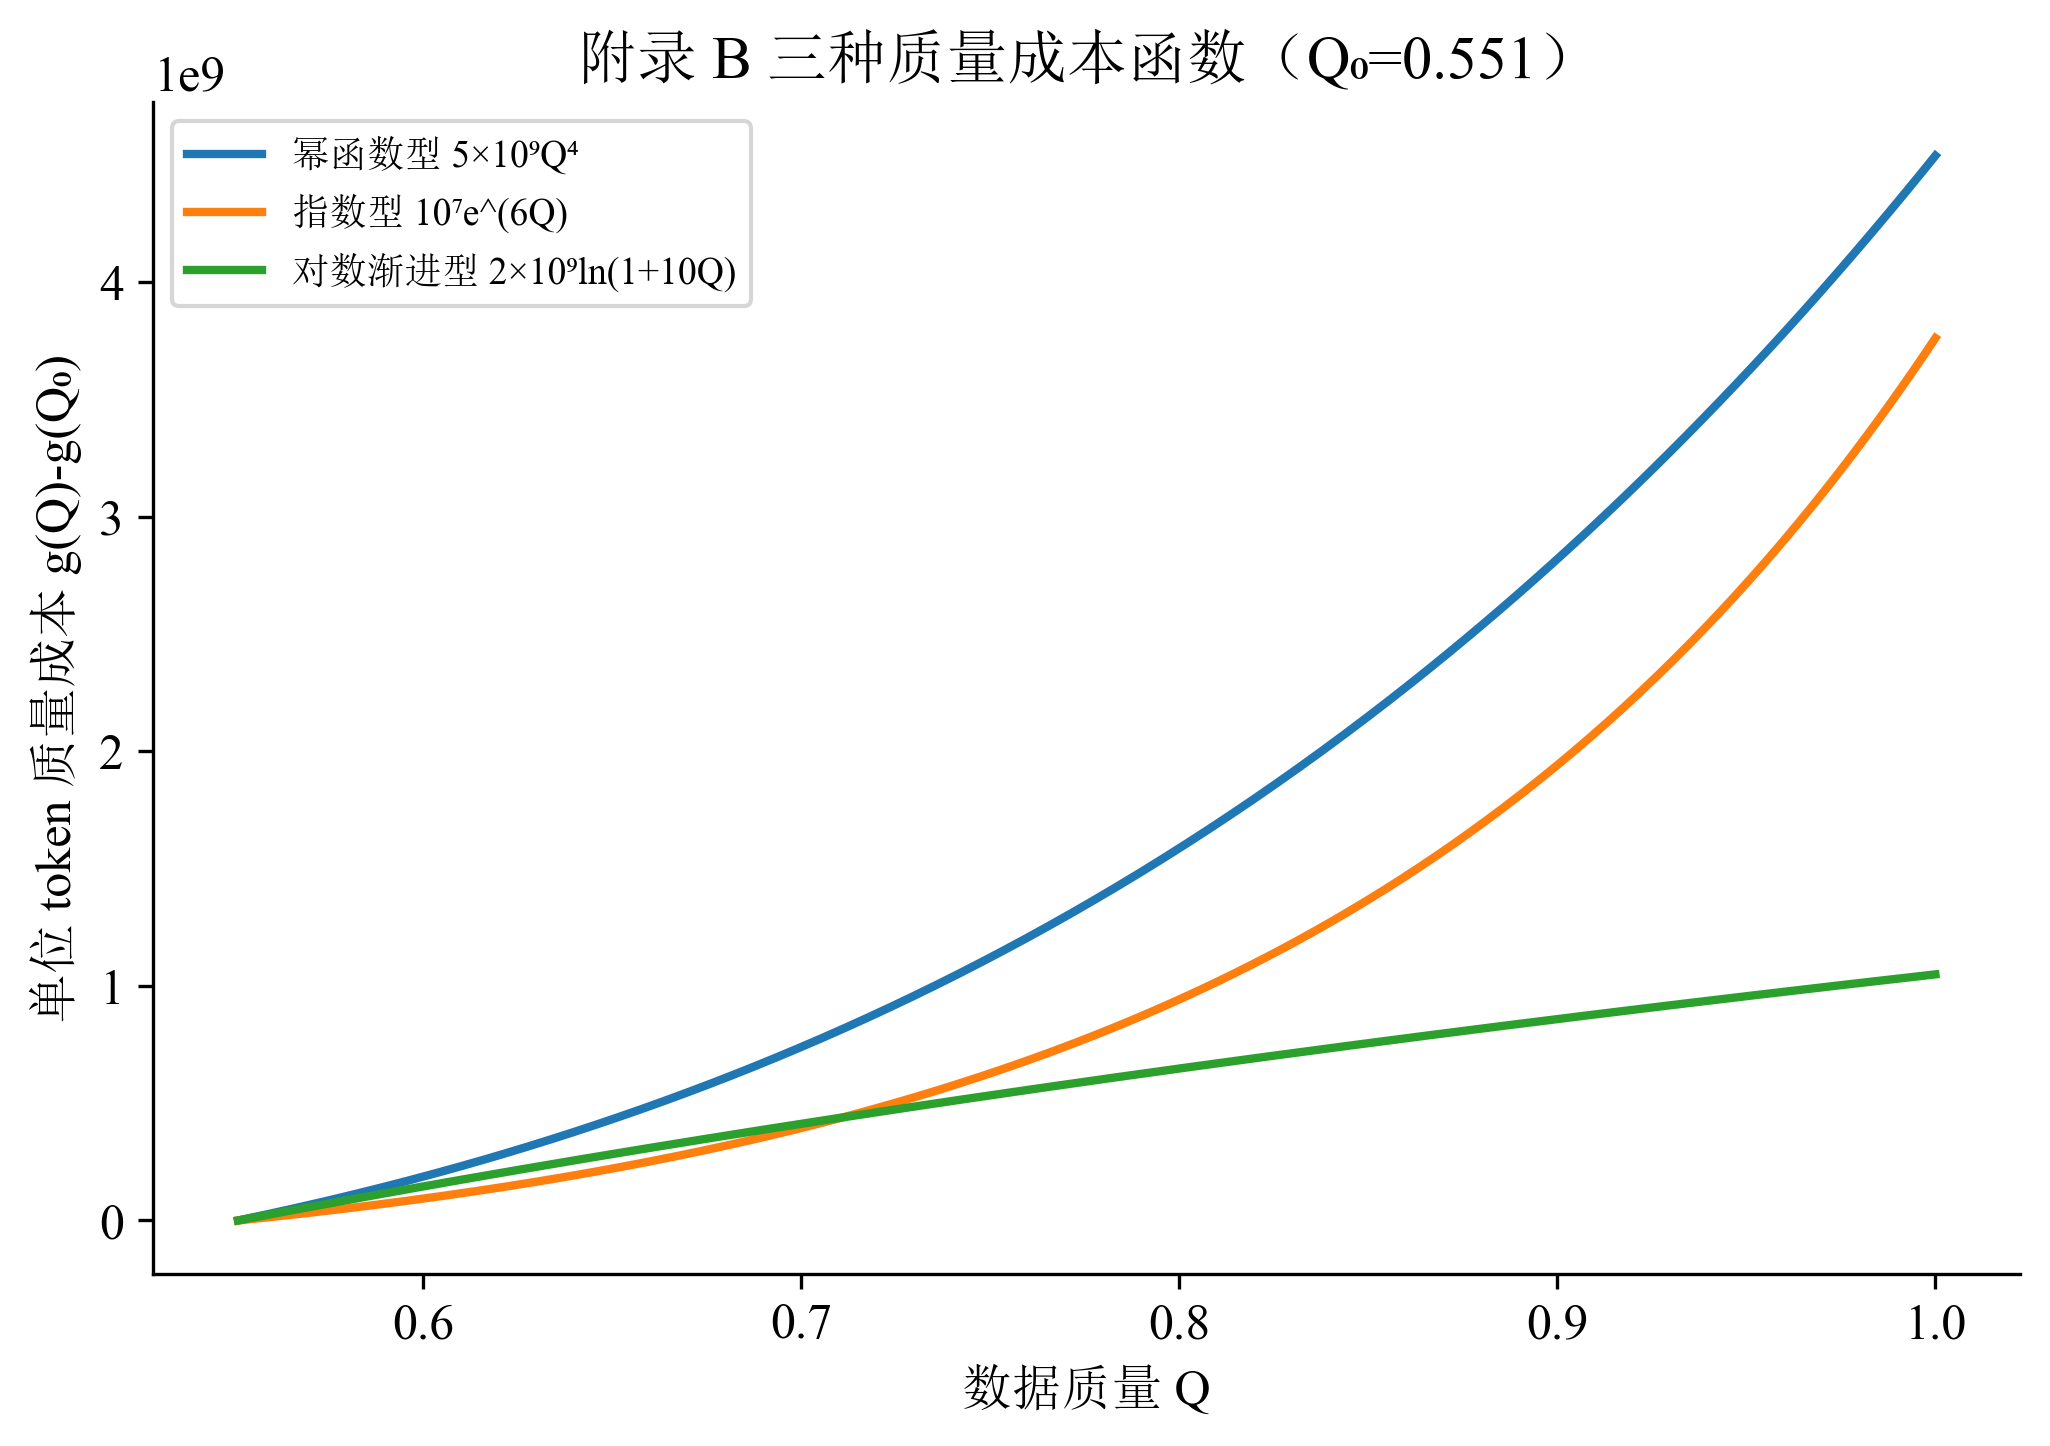
\includegraphics[width=0.62\textwidth]{求解/问题三/图片/图4_质量成本函数对比.png}
  \caption{附录 B 规定的三种质量成本函数（$Q_0=0.364$）}
  \label{fig:p3_cost}
\end{figure}

由表\ref{tab:p3_cost}与图\ref{fig:p3_cost}可知，成本函数的选择**只在最低预算档对最优质量有实质影响**（$Q^{*}$ 在 $0.551\sim1.000$ 之间，最优损失的差异仍小于 $0.06$）：对数渐进型在低预算下就愿意把质量做满（$Q^{*}=1.000$、质量份额 $31.6\%$），幂函数型则完全不投资质量（$Q^{*}=Q_0=0.551$、份额 $0$），指数型居中（$0.660$、$12.9\%$）。一旦预算达到 $10^{22}$ FLOPs 量级，三种成本函数下最优质量均达到上界 $1.000$，最优 $N$、$D$ 的差异在 $10\%$ 以内。这说明“中高预算下应优先把质量做满”的结论对成本函数形式稳健，而“低预算下是否投资质量”高度依赖具体成本函数设定，须谨慎表述。

\textbf{2.预算扫略与结构性转移识别}

预算扫略下最优质量与预算份额的演化如图\ref{fig:p3_shift}所示，结构性转移门槛见表\ref{tab:p3_shift}。

\begin{figure}[ht]
  \centering
  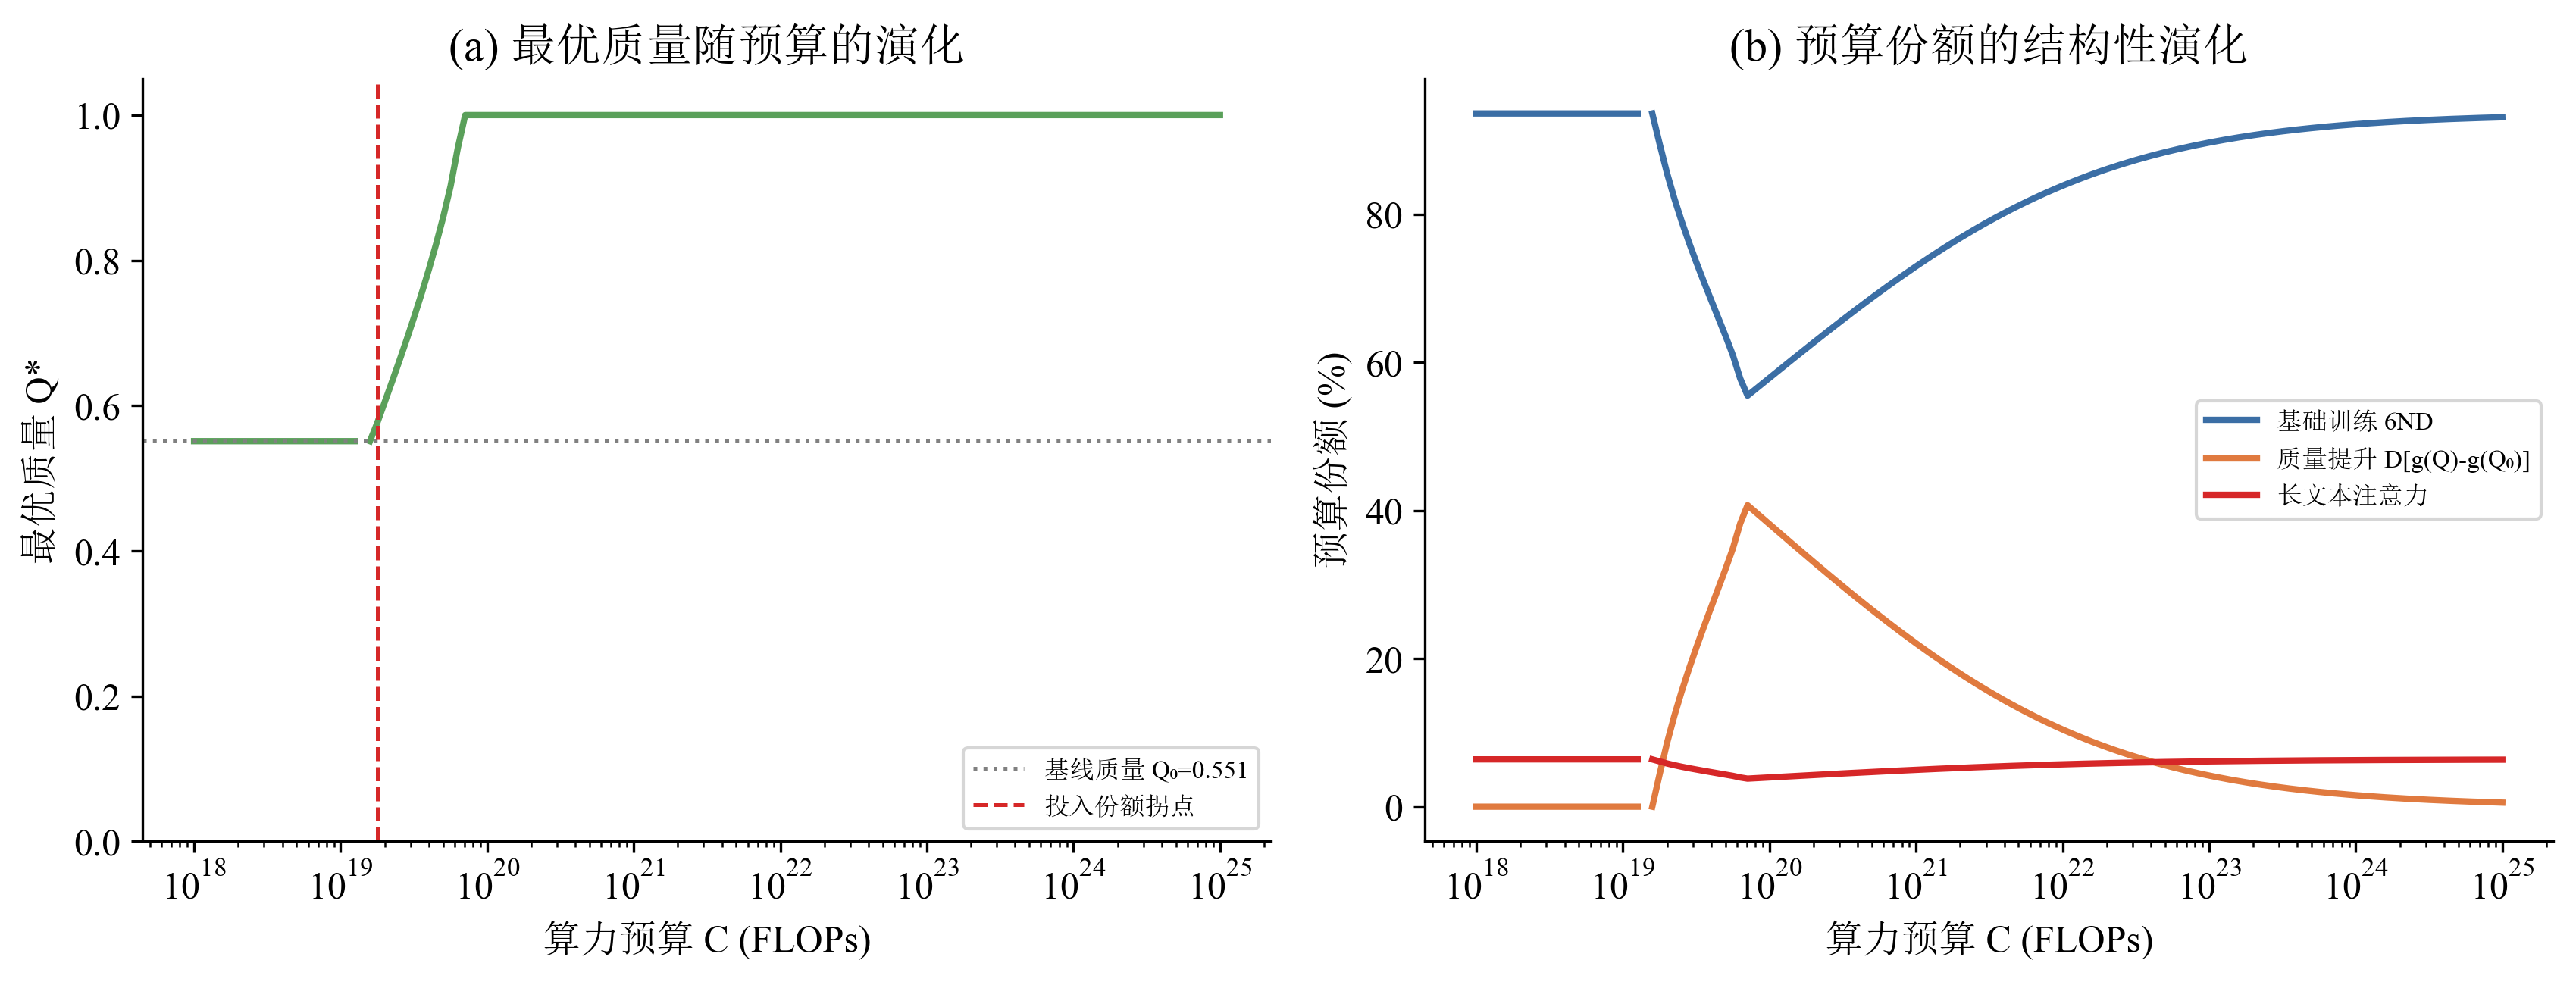
\includegraphics[width=0.92\textwidth]{求解/问题三/图片/图2_预算份额结构性转移.png}
  \caption{预算扫略下的资源配置结构性转移（左：最优质量演化；右：预算份额演化）}
  \label{fig:p3_shift}
\end{figure}

\begin{longtable}{>{\raggedright\arraybackslash}p{0.62\textwidth}>{\centering\arraybackslash}p{0.30\textwidth}}
  \caption{结构性转移门槛的定量识别}
  \label{tab:p3_shift} \\
  \toprule
  识别量 & 预算门槛（FLOPs） \\
  \midrule
  \endfirsthead
  \caption{结构性转移门槛的定量识别（续）} \\
  \toprule
  识别量 & 预算门槛（FLOPs） \\
  \midrule
  \endhead
  \bottomrule
  \endfoot
  制度一/二边界：质量投入启动（$\mathrm df_{\text{qual}}/\mathrm d\ln C$ 峰值，份额由 $0$ 转正） & $1.78\times10^{19}$ \\
  完成度 $\Theta$ 首次达到 $25\%$ & $2.82\times10^{19}$ \\
  完成度 $\Theta$ 首次达到 $50\%$ & $3.98\times10^{19}$ \\
  完成度 $\Theta$ 首次达到 $75\%$ & $5.62\times10^{19}$ \\
  质量提升完成度弹性 $\mathrm d\ln\Theta/\mathrm d\ln C$ 取得极大值 & $6.31\times10^{19}$ \\
  制度二/三边界：完成度 $\Theta$ 首次达到 $99\%$（质量接近饱和） & $7.08\times10^{19}$ \\
  质量投入份额峰值（$0.407$） & $7.08\times10^{19}$ \\
\end{longtable}

由表\ref{tab:p3_shift}与图\ref{fig:p3_shift}可知，预算路径被两个门槛切成三个制度，构成对结构性转移的直接证据：

\begin{itemize}[itemindent=2em]
\item \textbf{制度一（$C\lesssim1.78\times10^{19}$）：基线质量期。} 优化解取 $Q^{*}=Q_0$、质量份额恒为 $0$——算力紧张时最优策略是**放弃质量投入、把全部预算投向规模**；此时三项份额固定为训练 $93.6\%$、质量 $0\%$、注意力 $6.4\%$。
\item \textbf{制度二（$1.78\times10^{19}\lesssim C\lesssim1\times10^{20}$）：质量提升期。} 质量投入份额由 $0$ 迅速上升并在 $C=7.08\times10^{19}$ 处达到峰值 $0.407$，同期完成度 $\Theta$ 依次越过 $25\%$、$50\%$、$75\%$、$99\%$，其弹性在 $6.31\times10^{19}$ 处最大——这一阶段边际算力的首选去向是数据质量。
\item \textbf{制度三（$C\gtrsim1\times10^{20}$）：质量饱和期。} $Q^{*}$ 顶到上界 $1.000$ 后质量不再是可调节的边际资源，质量份额单调回落（$0.407\to0.006$），训练份额回升至 $93.1\%$，资源配置重新回到“以规模与数据为主”。
\end{itemize}

其经济学解释为：质量缺口惩罚 $C(1-Q)^{\gamma}$ 在低质量处对损失的边际压制最强，即 $|\partial L/\partial Q|$ 随 $Q$ 递减（见图\ref{fig:p2_margin}(b)），因此在质量尚未提升时投入质量最划算；而当 $Q$ 接近上界、边际收益趋零后，继续追加质量只是徒增成本，边际算力自然转向规模与数据。因此本问结论为：**预算跨越 $10^{19}\to10^{22}\to10^{24}$ 量级时，资源配置确实发生了质的变化——低预算制度“只扩规模、不投质量”，中等预算制度“优先把质量做满”，高预算制度“质量饱和后回归规模扩张”。**

\textbf{3.上下文长度敏感性（基于 C7 可行取值）}

在 $C=10^{22}$ FLOPs、幂函数型质量成本下，对附件 C7 的五个可行上下文长度逐一求解，结果见表\ref{tab:p3_ctx}与图\ref{fig:p3_ctx}。

\begin{longtable}{>{\centering\arraybackslash}p{0.13\textwidth}>{\centering\arraybackslash}p{0.13\textwidth}>{\centering\arraybackslash}p{0.13\textwidth}>{\centering\arraybackslash}p{0.13\textwidth}>{\centering\arraybackslash}p{0.11\textwidth}>{\centering\arraybackslash}p{0.11\textwidth}>{\raggedright\arraybackslash}p{0.14\textwidth}}
  \caption{上下文长度敏感性（$C=10^{22}$ FLOPs，幂函数型质量成本）}
  \label{tab:p3_ctx} \\
  \toprule
  $L_{\text{ctx}}$ & 注意力/训练 & $N^{*}$ (B) & $D^{*}$ (B) & $Q^{*}$ & $L^{*}$ & 注意力占比 \\
  \midrule
  \endfirsthead
  \caption{上下文长度敏感性（续）} \\
  \toprule
  $L_{\text{ctx}}$ & 注意力/训练 & $N^{*}$ (B) & $D^{*}$ (B) & $Q^{*}$ & $L^{*}$ & 注意力占比 \\
  \midrule
  \endhead
  \bottomrule
  \endfoot
  2{,}048 & 0.068 & 6.089 & 229.5 & 1.000 & 2.145 & 5.7\% \\
  4{,}096 & 0.137 & 5.897 & 223.5 & 1.000 & 2.149 & 10.8\% \\
  8{,}192 & 0.273 & 5.562 & 212.7 & 1.000 & 2.157 & 19.4\% \\
  32{,}768（超临界） & 1.092 & 4.318 & 170.2 & 1.000 & 2.194 & 48.2\% \\
  131{,}072（超临界） & 4.369 & 2.705 & 109.1 & 1.000 & 2.273 & 77.3\% \\
\end{longtable}

\begin{figure}[ht]
  \centering
  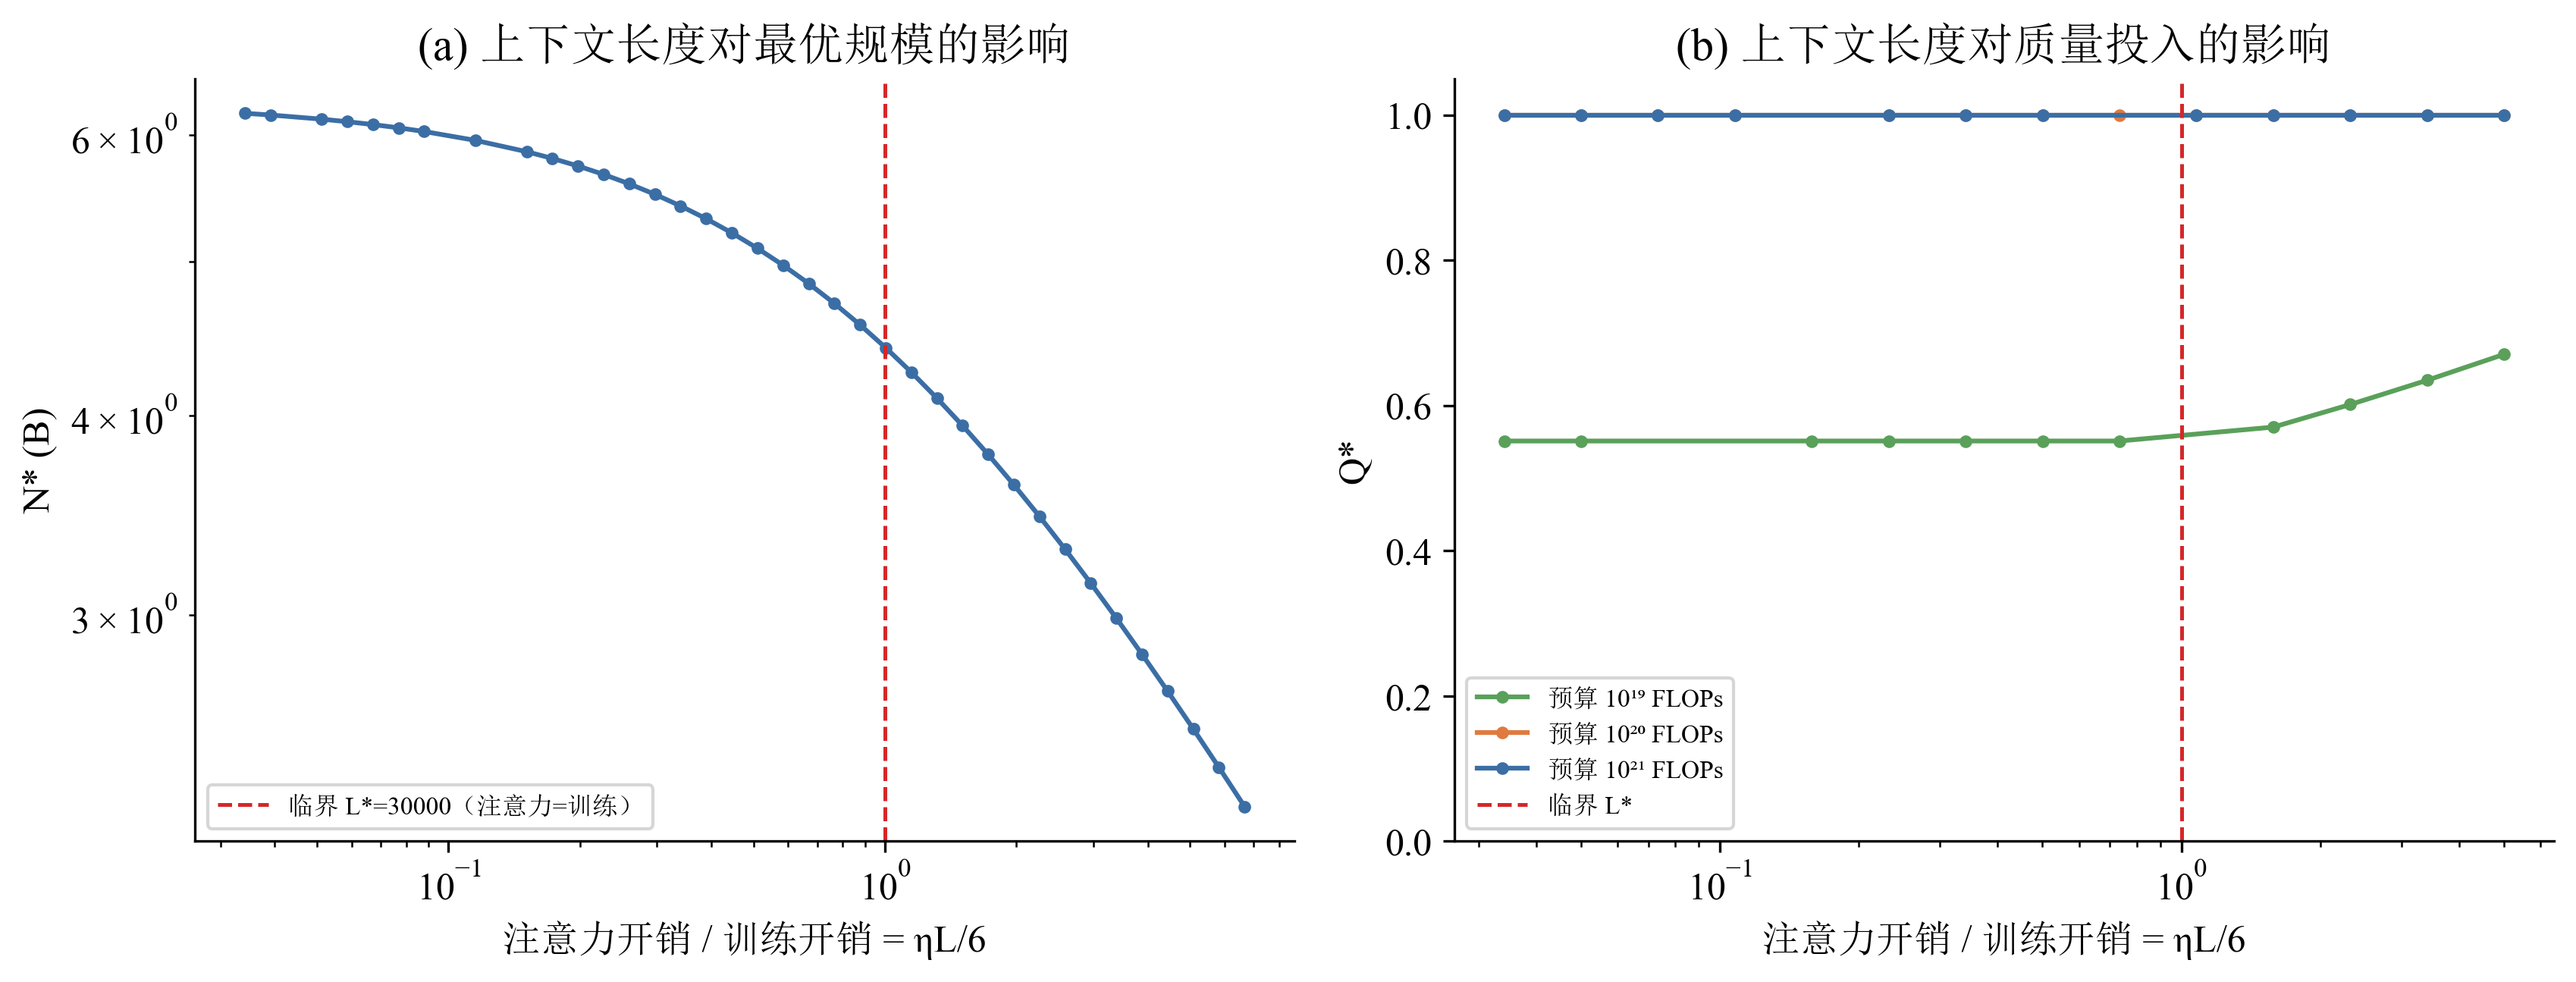
\includegraphics[width=0.92\textwidth]{求解/问题三/图片/图3_上下文长度敏感性.png}
  \caption{上下文长度敏感性（左：注意力开销对最优规模的影响；右：对质量投入的影响）}
  \label{fig:p3_ctx}
\end{figure}

由表\ref{tab:p3_ctx}可知，C7 的五个可行取值恰好跨越临界值 $L_{\text{crit}}=30{,}000$：$8{,}192$ tokens 时注意力开销仅为训练开销的 $0.273$ 倍，而 $32{,}768$ tokens 时已达 $1.092$ 倍、超过临界点。随上下文长度增长，注意力开销占比由 $5.7\%$ 升至 $77.3\%$，最优参数量被压缩 $2.25$ 倍、最优数据量被压缩 $2.10$ 倍，最优损失上升 $0.128$（约 $6.0\%$）。这一结论量化了“长上下文与规模投入存在算力竞争”的直觉：由于 $N^*\propto C^{\beta/(\alpha+\beta)}$，当基础训练单价被放大 $1+\lambda$ 倍时，可用于规模的等效预算按 $(1+\lambda)^{-\beta/(\alpha+\beta)}$ 缩减。需要说明的是，在 $C=10^{22}$ 这一预算档，即使 $L_{\text{ctx}}=131{,}072$，最优质量仍达上界 $1.000$，即长上下文的挤压主要体现在规模而非质量上——这与表\ref{tab:p3_shift}所示“中高预算下质量已饱和”的判断一致。

一个容易被直觉忽略的现象是：在**低预算档**，注意力开销上升反而使最优质量**提高**（图\ref{fig:p3_ctx}(b) 中 $C=10^{19}$ 曲线在 $L_{\text{ctx}}$ 由 $1{,}024$ 增至 $150{,}000$、注意力开销倍数由 $0.03$ 增至 $5.0$ 时，$Q^{*}$ 由 $0.551$（=基线，不投资质量）升至 $0.670$）。原因是本模型严格保留了赛题给定的“质量成本与训练 token 数成正比”结构 $C_Q=D[g(Q)-g(Q_0)]_+$：长上下文挤压了可负担的数据量 $D$，而 $D$ 越小，把整份语料提升到质量 $Q$ 的总开销越低，于是质量投入的相对价格下降、最优质量上移。这提示在真实训练中，长上下文与数据质量投入并非简单互斥，而是通过数据规模这一中间变量发生耦合——若采用“质量成本与数据量无关”的简化假设，这一耦合将被完全抹掉。

\textbf{4.领域配比的算力等价效果}

将问题一的推荐配比（$M=-0.1988$）与参考配比（$M=0$）在 $C=10^{22}$ FLOPs 下对比：两种情形的最优 $(N^{*},D^{*},Q^{*})$ 完全相同，但最优损失由 $2.1450$ 降至 $1.9462$。进一步用二分法求“参考配比达到同一损失所需的预算”，得 $C\approx3.05\times10^{23}$ FLOPs，即**领域配比优化的效果相当于约 $30$ 倍的算力扩张**。这为“调整领域配比虽不增加算力总开销，却会显著改变算力的使用效果”提供了定量证据。需说明的是，$M(\bm p)$ 是损失水平上的固定平移、与算力无关，因此换算为算力收益时会被损失的算力弹性放大，该倍数宜作量级参考而非精确比值。

综合以上结果，本节完成了问题三的求解：严格按赛题公式建立了含基础训练、质量提升与长文本注意力的成本模型，解析给出临界上下文长度 $L_{\text{crit}}=30{,}000$ tokens，求得三档预算下的最优资源配置，并以“质量投入启动边界 $1.78\times10^{19}$”与“质量接近饱和边界 $7.08\times10^{19}$”两个门槛识别出\textbf{基线质量期 $\to$ 质量提升期 $\to$ 质量饱和期}的三段式结构性转移。

\subsection{问题四的模型的建立和求解}

\subsubsection{具体分析}

针对问题四，本问属于\textbf{技术演进建模与前沿预测}类问题，需要结合历史评测数据建立技术演进模型，分离并量化规模扩张与非规模技术进步的贡献占比，并预测未来 12 至 24 个月开源大语言模型能力的前沿边界\cite{wei2022emergent}。本问综合采用“口径界定 $\to$ Loss—Benchmark 桥接 $\to$ 面板回归分解 $\to$ 前沿预测 $\to$ 宏观证据校验”五步框架：首先明确综合能力的度量方式、开源筛选口径、模型类型口径与时间轴口径；再按可比性分层建立交叉熵损失与 Leaderboard 得分的映射，把前三问以损失为目标的结论桥接到以评测得分为度量的能力；然后以参数规模与年份为解释变量做面板回归（含年份固定效应），把能力提升分解为“规模扩张”与“非规模技术进步”两部分；接着用 logistic 饱和模型与结构外推两条路线给出未来 12/24 个月的前沿预测与不确定性区间；最后用附件 C4 的算力、数据量与开源权重证据检验“算力增长放缓”情景的合理性。

本问严格完成题设的必用要求：对 C8 的逐任务评测 JSON 做逐任务聚合分析（不依赖汇总表），对 C4 的算力、数据量与开源权重字段作宏观证据检验，桥接数据按可比性等级（C6 的 High/Medium，并以 C5 对照）分层使用。

\subsubsection{模型准备}

\textbf{1.口径界定}

\textbf{（1）综合能力度量。} 采用 Open LLM Leaderboard v2 的六维平均分 $\bar B$：IFEval（指令遵循）、BBH（多跳推理）、MATH Lvl 5（数学）、GPQA（研究生级问答）、MUSR（多轮推理）、MMLU-PRO（专业知识）。六维等权平均，取值 $0\sim100$。

\textbf{（2）时间轴口径。} 统一以 C1 的 Submission Date（提交日期）为基准，并按“年 $+$ 月”折算为连续时间变量 $t=\text{年份}-2019+(\text{月}-0.5)/12$。之所以不采用发布日期或版本日期，是因为 Leaderboard 上的评测结果均在提交时冻结、且提交日期字段完整无缺失；C3 的 Year 字段仅用于 2019--2023 的历史锚点对照。

\textbf{（3）开源筛选口径。} 同时要求两个条件：（a）模型权重可获取（Type 属 pretrained、持续预训练、chat、域内微调四类）；（b）Hub License 允许研究与复现，即采用 apache-2.0、mit、gpl-3.0、cc-by-4.0、mpl-2.0、bsd-3-clause、llama2/3/3.1/3.2/3.3、gemma、cc-by-sa-4.0、openrail 等许可，排除 cc-by-nc 系列（非商用）、creativeml-openrail、bigscience-bloom-rail 等受限许可以及未知许可。筛选漏斗见表\ref{tab:p4_funnel}。

\textbf{（4）模型类型口径。} 明确区分 pretrained（含持续预训练，共 231 条）与 chat/finetuned（经对话指令或监督微调，共 1{,}497 条）两类，分组统计规模效应与时间效应；base 合并模型（1{,}724 条，非独立训练过程）与多模态模型（9 条，任务构成不同）不并入主分析。

\begin{longtable}{>{\raggedright\arraybackslash}p{0.56\textwidth}>{\centering\arraybackslash}p{0.16\textwidth}>{\raggedright\arraybackslash}p{0.22\textwidth}}
  \caption{数据筛选漏斗（C1 排行榜）}
  \label{tab:p4_funnel} \\
  \toprule
  筛选层级 & 记录数 & 说明 \\
  \midrule
  \endfirsthead
  \caption{数据筛选漏斗（续）} \\
  \toprule
  筛选层级 & 记录数 & 说明 \\
  \midrule
  \endhead
  \bottomrule
  \endfoot
  C1 全量记录 & 4{,}576 & 提交日期 2024-06-08 $\sim$ 2025-03-13 \\
  六维得分完整 & 4{,}576 & 无缺失 \\
  时间/参数/六维齐备 & 4{,}561 & 剔除 15 条参数或日期缺失 \\
  许可允许研究复现（开源口径） & 2{,}346 & 符合上述许可白名单 \\
  其中 pretrained & 231 & 类型为 pretrained / 持续预训练 \\
  其中 chat/finetuned & 1{,}497 & 类型为 chat / 域内微调 \\
\end{longtable}

\textbf{2.附件 C8 的逐任务聚合}

附件 C8 含 1{,}863 个模型子目录、1{,}958 个评测 JSON。本文按目录取最新可解析记录，提取每个模型在各任务上的原始指标（按 acc\_norm、acc、prompt\_level\_loose\_acc、inst\_level\_loose\_acc、exact\_match 的优先级选取），共成功解析 1{,}860 个模型，跳过 7 个损坏或无有效记录的目录。解析后可用的子任务维度共 37 项：BBH 子任务 24 项、MATH-Hard 子任务 7 项、GPQA 子集 3 项、MUSR 子任务 3 项。

由于 C8 保存的是原始指标、而 C1 保存的是官方按随机基线归一化后的六维得分（例如 $\text{GPQA}=(\text{raw}-0.25)/0.75$、$\text{MMLU-PRO}=(\text{raw}-0.10)/0.90$、$\text{IFEval}=(\text{prompt\_strict}+\text{inst\_strict})/2$），两者存在系统性水平差。因此本文的处理是：跨模型得分分析使用 C1，逐任务结构分析在 C8 的原始指标空间内进行，并以秩相关作为两者的衔接验证，结果见表\ref{tab:p4_c8chk}。

\begin{longtable}{>{\centering\arraybackslash}p{0.22\textwidth}>{\centering\arraybackslash}p{0.16\textwidth}>{\centering\arraybackslash}p{0.16\textwidth}>{\centering\arraybackslash}p{0.16\textwidth}>{\raggedright\arraybackslash}p{0.22\textwidth}}
  \caption{C8 解析结果与 C1 的一致性校验}
  \label{tab:p4_c8chk} \\
  \toprule
  任务 & 匹配模型数 & Pearson $r$ & Spearman $\rho$ & 平均绝对偏差 \\
  \midrule
  \endfirsthead
  \caption{C8 与 C1 一致性校验（续）} \\
  \toprule
  任务 & 匹配模型数 & Pearson $r$ & Spearman $\rho$ & 平均绝对偏差 \\
  \midrule
  \endhead
  \bottomrule
  \endfoot
  IFEval & 1{,}896 & 0.987 & 0.987 & 2.88 \\
  BBH & 1{,}898 & 0.998 & 0.997 & 21.06 \\
  MATH Lvl 5 & 1{,}897 & 0.803 & 0.812 & 3.47 \\
  GPQA & 1{,}894 & 0.987 & 0.992 & 23.38 \\
  MUSR & 1{,}894 & 0.973 & 0.977 & 30.73 \\
  MMLU-PRO & 1{,}896 & 0.998 & 0.998 & 7.56 \\
\end{longtable}

由表\ref{tab:p4_c8chk}可知，两套数据的秩一致性均在 $0.81$ 以上（多数在 $0.97$ 以上），说明 C8 的逐任务解析结果与官方汇总得分反映同一批评测；平均绝对偏差较大的维度（GPQA 23.4、MUSR 30.7、BBH 21.1）正是“原始分”与“基线归一化分”差异最大的维度，与前述口径说明完全对应。这一校验保证了后续逐任务结论的可靠性。

\textbf{3.算法选择}

Loss—Benchmark 映射采用按可比性分层的线性最小二乘（并在全样本上给出整体拟合），分层可避免“同模型同验证集”与“跨族近似验证集”样本混用造成的偏置；规模/时间分解同时采用线性时间 OLS 与年份固定效应两种设定，后者把非规模技术进步完全交由年效应吸收，可显著缓解规模与年份的共线性；前沿外推同时采用 logistic 饱和模型（有界、符合满分 100 的物理约束）与结构外推（把分解方程直接用作预测方程），两条路线互为校验；不确定性由残差 bootstrap（600 次重抽样）与情景分析共同给出。

\subsubsection{模型建立}

\textbf{步骤1：Loss—Benchmark 映射模型}

设验证损失 $L$ 与 Leaderboard 均分 $\bar B$ 之间存在近似线性关系：
\begin{equation}
    \bar B = a + b\,L
\end{equation}
系数 $a$、$b$ 由最小二乘估计，并按 C6 的 Loss\_Comparability 字段分为“高可比”（同模型同验证集，主要来自 Pythia，可与附件 B 对照）与“中可比”（Loss 来自不同技术报告或论文）两层分别估计。映射误差对结论的影响通过分层的 $R^2$、MAPE 与相关系数共同刻画。

\textbf{步骤2：规模扩张与技术进步分解模型}

以参数量对数与时间为解释变量建立面板回归：
\begin{equation}
    \text{Score}_{it} = b_0 + b_P\log_{10}P_{it} + b_t\,t + \varepsilon_{it}
    \qquad\text{或}\qquad
    \text{Score}_{it} = \alpha_t + b_P\log_{10}P_{it} + \varepsilon_{it}
\end{equation}
其中 $b_P$ 为规模系数（参数量每增大 10 倍带来的得分提升），$b_t$ 为时间系数（每年非规模技术进步带来的得分提升），$\alpha_t$ 为年份固定效应。前沿提升的 shift-share 分解为
\begin{equation}
    \Delta F = \underbrace{b_P\,\Delta\log_{10}P_{\text{frontier}}}_{\text{规模扩张贡献}}
    + \underbrace{\left[\Delta F - b_P\,\Delta\log_{10}P_{\text{frontier}}\right]}_{\text{非规模技术进步贡献}}
\end{equation}
两者占比即为所求贡献份额。$\Delta\log_{10}P_{\text{frontier}}$ 取各年“参数量最大的开放权重模型”的对数差，$\Delta F$ 取累计前沿（按定义单调不减）之差。

\textbf{步骤3：能力前沿预测模型（两条路线）}

\emph{路线一（曲线外推）}：能力前沿随时间的演化以 logistic 饱和函数刻画，并用残差 bootstrap 给出区间：
\begin{equation}
    F(t) = \frac{K}{1+e^{-r(t-t_0)}},\qquad K \text{ 为饱和上界},\ r \text{ 为增长率},\ t_0 \text{ 为拐点}
\end{equation}
前沿序列取“年度累计最大”与“月度前 $1\%$ 均值累计最大”拼接而成的单调不减序列。算力增长放缓情景以“增速减半”实现：
\begin{equation}
    F_{\text{slow}}(t)=K\left[1+e^{-r(\min(t,t_h)-t_0)}\right]^{-1},\qquad t_h \text{ 为增速减半时刻}
\end{equation}

\emph{路线二（结构外推）}：直接把分解方程用作预测方程，
\begin{equation}
    \hat F(t+\Delta) = F(t) + \left[b_P\,\Delta\log_{10}P + b_t\right]\cdot\Delta
\end{equation}
并按“前沿模型规模持平（$\Delta\log_{10}P=0$）”“算力增长放缓（$b_t$ 减半）”“规模继续扩张（$\Delta\log_{10}P=+0.3$/年）”三种情景给出区间。

\subsubsection{模型求解}

\textbf{1.Loss—Benchmark 桥接结果}

映射结果如图\ref{fig:p4_map}所示，分层拟合结果如表\ref{tab:p4_bridge}所示。

\begin{figure}[ht]
  \centering
  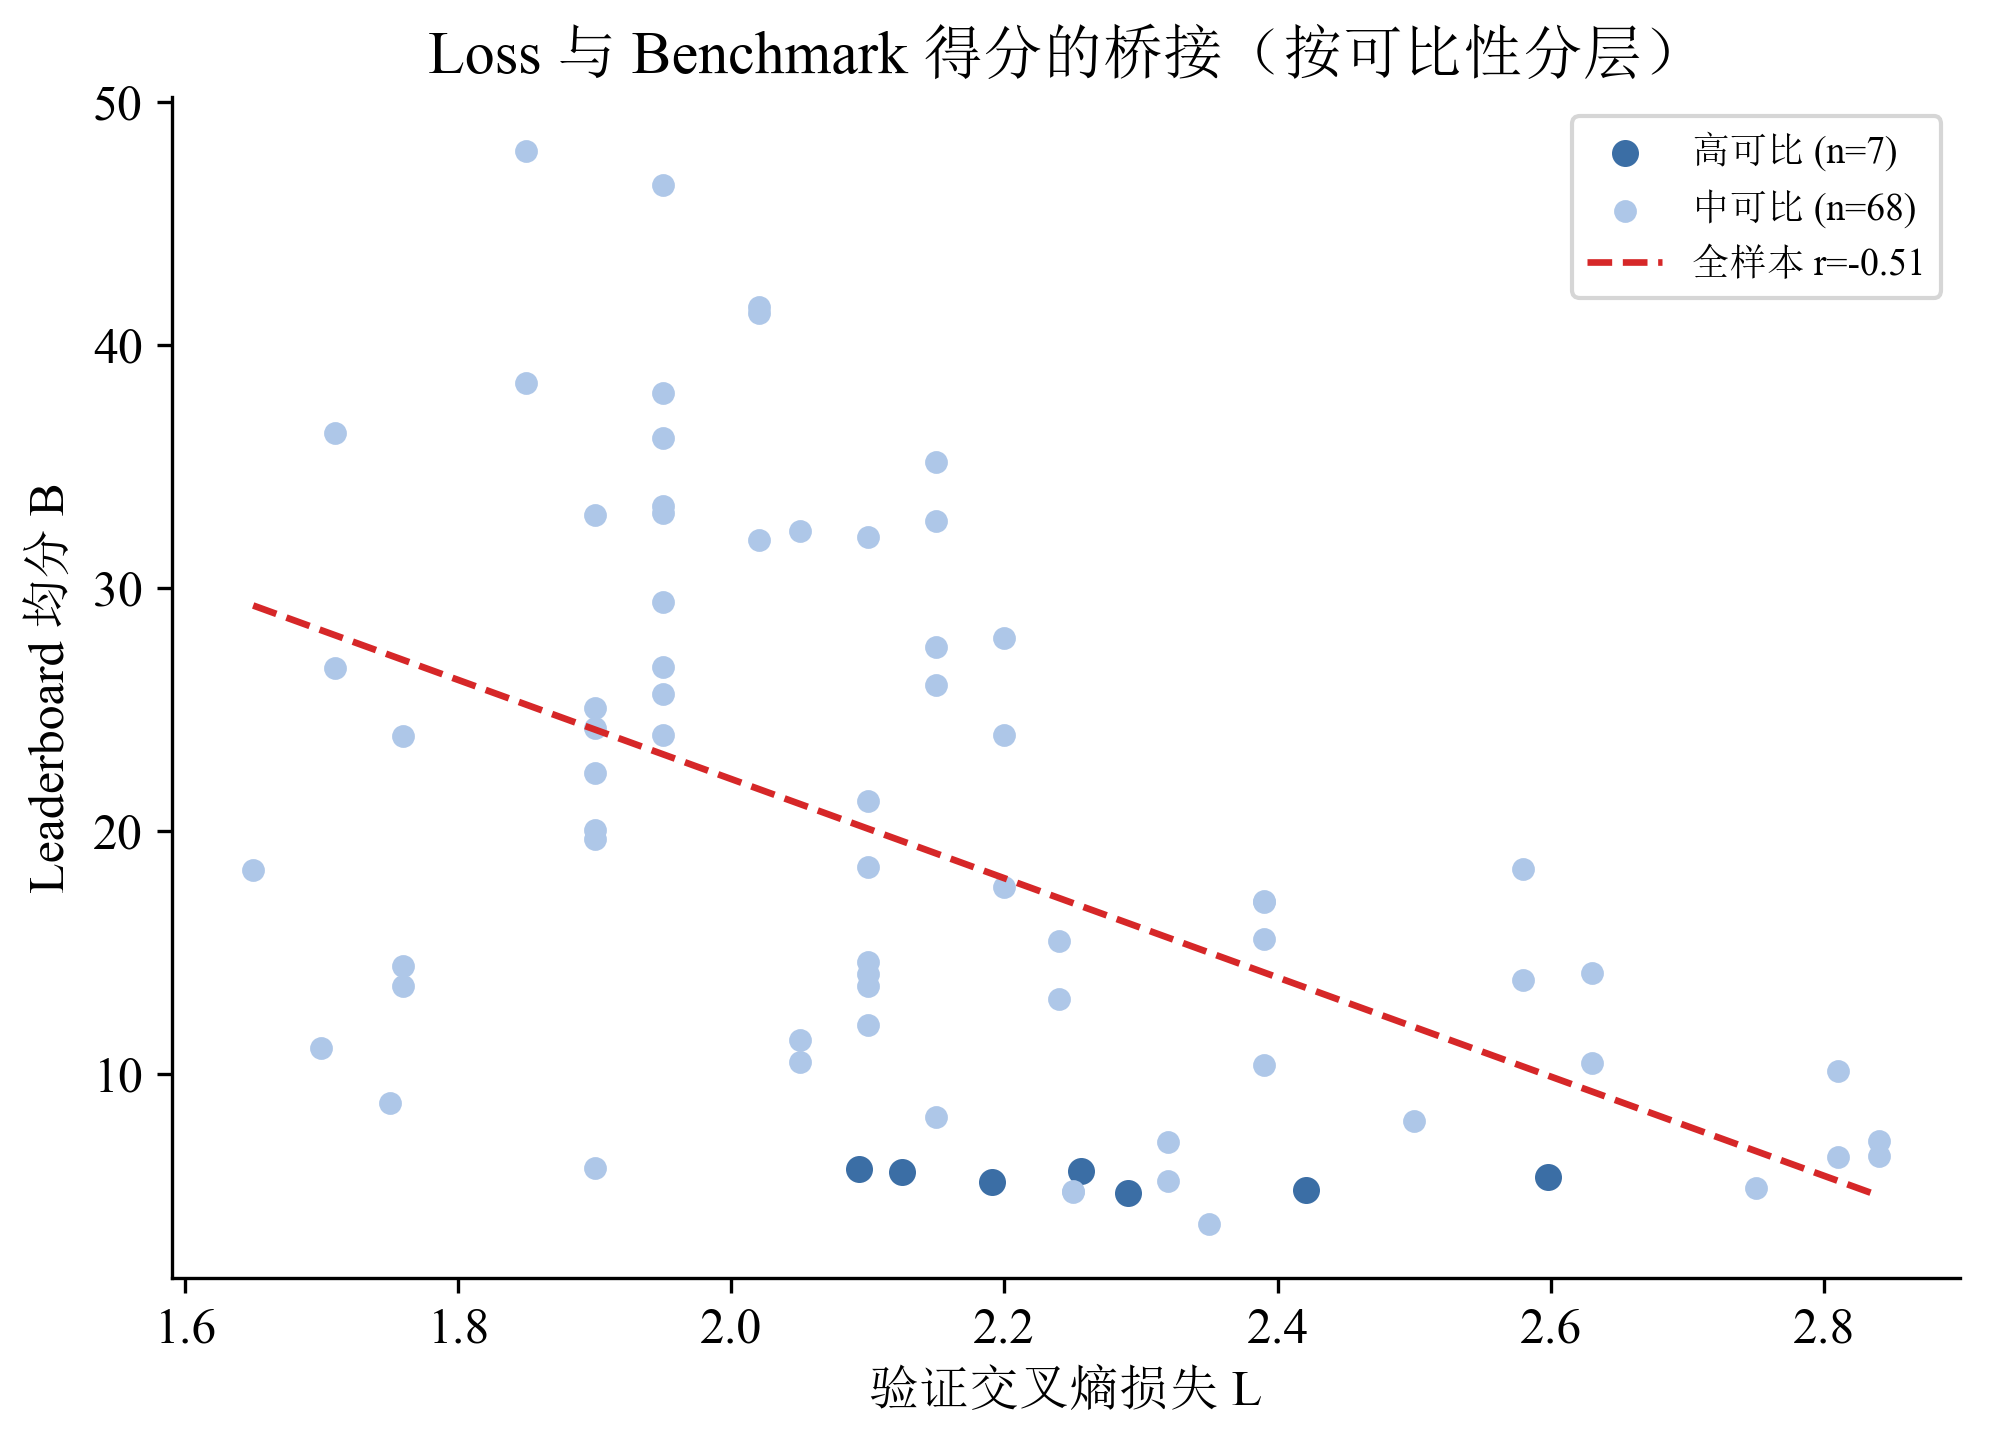
\includegraphics[width=0.60\textwidth]{求解/问题四/图片/图1_Loss_Benchmark映射.png}
  \caption{验证损失与 Leaderboard 均分的映射关系（按可比性分层）}
  \label{fig:p4_map}
\end{figure}

\begin{longtable}{>{\centering\arraybackslash}p{0.16\textwidth}>{\centering\arraybackslash}p{0.10\textwidth}>{\centering\arraybackslash}p{0.13\textwidth}>{\centering\arraybackslash}p{0.13\textwidth}>{\centering\arraybackslash}p{0.13\textwidth}>{\centering\arraybackslash}p{0.10\textwidth}>{\raggedright\arraybackslash}p{0.14\textwidth}}
  \caption{Loss—Benchmark 映射的分层拟合结果（C6，$n=75$）}
  \label{tab:p4_bridge} \\
  \toprule
  可比性 & $n$ & Pearson $r$ & Spearman $\rho$ & 斜率 $b$ & $R^2$ & MAPE(\%) \\
  \midrule
  \endfirsthead
  \caption{Loss—Benchmark 映射的分层拟合结果（续）} \\
  \toprule
  可比性 & $n$ & Pearson $r$ & Spearman $\rho$ & 斜率 $b$ & $R^2$ & MAPE(\%) \\
  \midrule
  \endhead
  \bottomrule
  \endfoot
  高可比 & 7 & $-0.397$ & $-0.607$ & $-0.882$ & 0.16 & 5.6 \\
  中可比 & 68 & $-0.502$ & $-0.509$ & $-19.185$ & 0.25 & 57.3 \\
  全样本 & 75 & $-0.510$ & $-0.549$ & $-20.417$ & 0.26 & 67.8 \\
  C5 对照（全样本） & 43 & $-0.502$ & — & $-16.155$ & — & — \\
\end{longtable}

由表\ref{tab:p4_bridge}可知：（1）损失与能力得分确实负相关（全样本 $r=-0.510$，Spearman $\rho=-0.549$，$p<10^{-6}$），验证了“以损失为目标的资源配置可转化为能力收益”的桥接逻辑；（2）但映射的 $R^2$ 仅 $0.26$、MAPE 高达 $67.8\%$，说明桥接关系是弱关系，其原因是中可比样本的 Loss 来自不同论文的不同验证集、量纲不完全统一；（3）高可比子集（Pythia 同模型同验证集）的斜率最缓（$-0.882$）、MAPE 最低（$5.6\%$），但其得分变化幅度极小（$5.07\sim6.06$），因为这些小规模基础模型在六维基准上都接近随机水平，损失的大幅下降并未转化为得分提升。因此本文的桥接结论仅用于方向性判定与量级估计，不用于把损失数值精确换算为得分。

\textbf{2.规模扩张与非规模技术进步的贡献分解}

面板回归结果见表\ref{tab:p4_panel}，贡献分解如图\ref{fig:p4_decomp}所示。

\begin{longtable}{>{\raggedright\arraybackslash}p{0.28\textwidth}>{\centering\arraybackslash}p{0.10\textwidth}>{\centering\arraybackslash}p{0.14\textwidth}>{\centering\arraybackslash}p{0.12\textwidth}>{\centering\arraybackslash}p{0.10\textwidth}>{\raggedright\arraybackslash}p{0.18\textwidth}}
  \caption{规模系数估计（C1 开源筛选样本，2{,}346 条，2024--2025 年）}
  \label{tab:p4_panel} \\
  \toprule
  子样本 & $n$ & $b_P$（分/10 倍参数） & $b_t$（分/年） & $R^2$ & 说明 \\
  \midrule
  \endfirsthead
  \caption{规模系数估计（续）} \\
  \toprule
  子样本 & $n$ & $b_P$（分/10 倍参数） & $b_t$（分/年） & $R^2$ & 说明 \\
  \midrule
  \endhead
  \bottomrule
  \endfoot
  全样本（年份固定效应） & 2{,}346 & 13.842 & — & 0.475 & 年效应吸收非规模进步 \\
  全样本（线性时间 OLS） & 2{,}346 & 13.842 & 4.844 & 0.475 & 两设定结果一致 \\
  pretrained & 231 & 6.414 & 1.552 & 0.460 & 基础模型 \\
  chat/finetuned & 1{,}497 & 14.853 & 4.680 & 0.484 & 指令/微调模型 \\
\end{longtable}

\begin{figure}[ht]
  \centering
  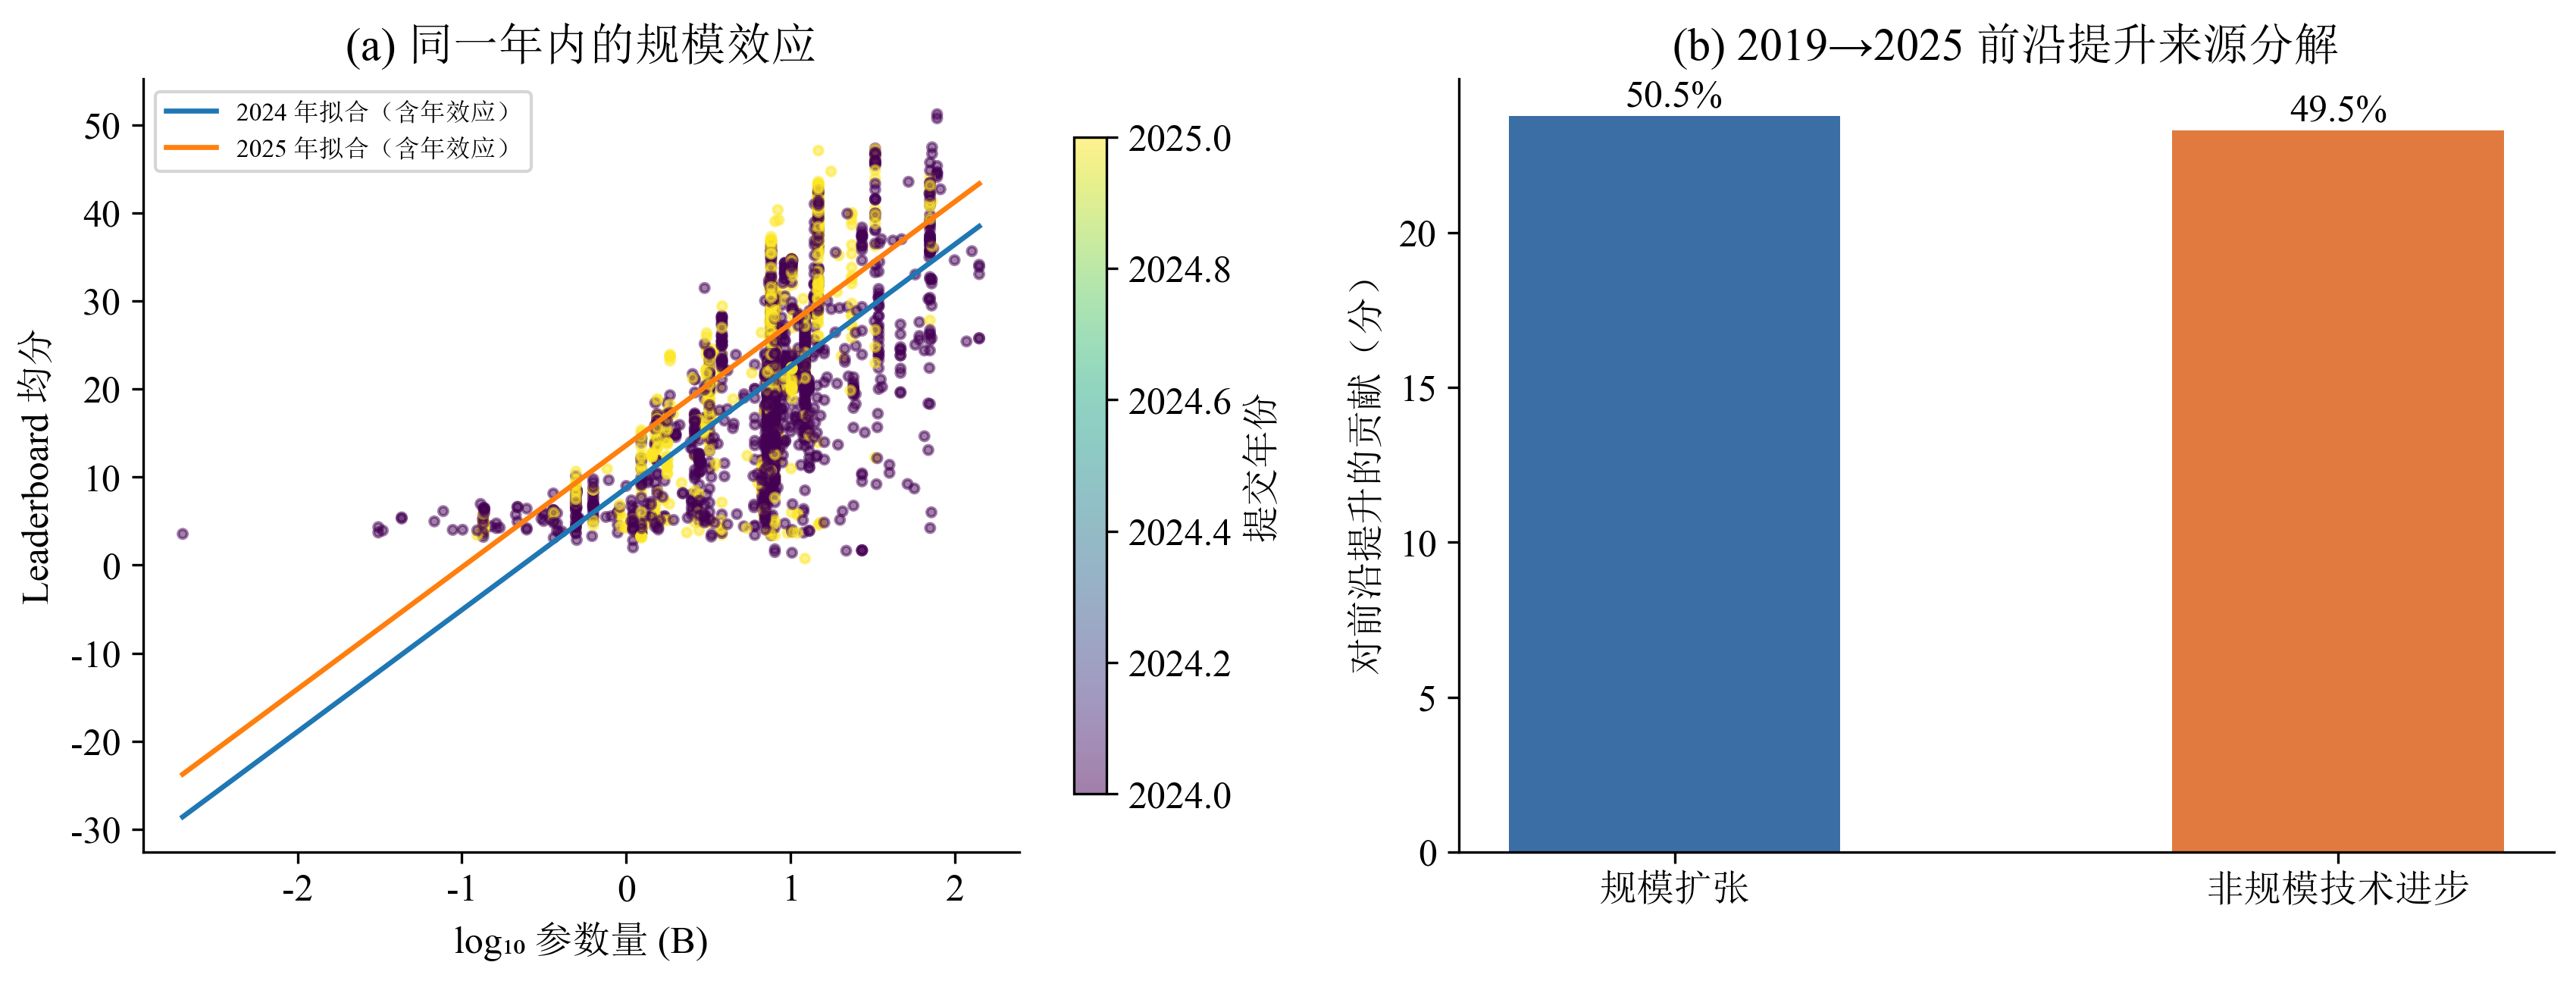
\includegraphics[width=0.92\textwidth]{求解/问题四/图片/图2_规模时间分解.png}
  \caption{规模效应与前沿提升来源分解（左：同一年内的规模效应；右：长周期贡献分解）}
  \label{fig:p4_decomp}
\end{figure}

由表\ref{tab:p4_panel}可知：（1）规模系数 $b_P=13.84$，即参数量每增大 10 倍，六维平均分提升约 $13.8$ 分；非规模技术进步速率 $b_t=4.84$ 分/年。（2）模型类型差异显著：pretrained 子样本的规模系数仅 $6.41$、时间系数 $1.55$，而 chat/finetuned 子样本达 $14.85$ 与 $4.68$，说明经指令微调对齐后的模型对参数规模的利用效率更高，基础模型在同一评测上的得分提升要慢得多。这提示在讨论“规模扩张 vs 技术进步”时必须区分模型类型，否则会因样本构成变化而混淆两者。

在长周期口径（C3，2019--2025）上，以 $b_P=14.10$、$b_t=3.30$（$R^2=0.42$）做 shift-share 分解：前沿由 $5.00$ 升至 $52.08$（提升 $47.08$ 分），其中 $b_P\Delta\log_{10}P=23.77$ 分、残差部分 $23.31$ 分，即\textbf{规模扩张贡献 $50.5\%$、非规模技术进步贡献 $49.5\%$}，二者几乎平分秋色。

但需指出长周期锚点存在口径风险。本文对 C3 做了自洽性审计：比较每行 Average 与其六维均值，发现 13 条记录的差值超过 5（最大差值 $42.3$，为 GPT-3 (175B) 的 Average $=50.0$ 而六维均值仅 $7.67$），说明这些历史条目混入了不同评测标准，已予以剔除。剔除后，在评测标准完全一致的近端窗口（2024-06 至 2024-09，前沿由 $37.99$ 升至 $51.00$）内分解得：前沿模型参数量仅由 $70.6$B 增至 $78.0$B（$\Delta\log_{10}P=0.043$），规模贡献 $0.60$ 分、非规模贡献 $12.41$ 分，即\textbf{该窗口内前沿提升的 $95.4\%$ 来自非规模因素}。这与长周期口径的 $50.5\%$ 形成互补：长期看规模与技术进步各贡献约一半，但在最近一年、模型规模趋于稳定的条件下，能力提升主要由数据工程、对齐方法等非规模因素驱动。

\textbf{3.能力前沿预测}

前沿序列与 logistic 拟合如图\ref{fig:p4_frontier}所示，预测结果与不确定性见表\ref{tab:p4_frontier}。

\begin{figure}[ht]
  \centering
  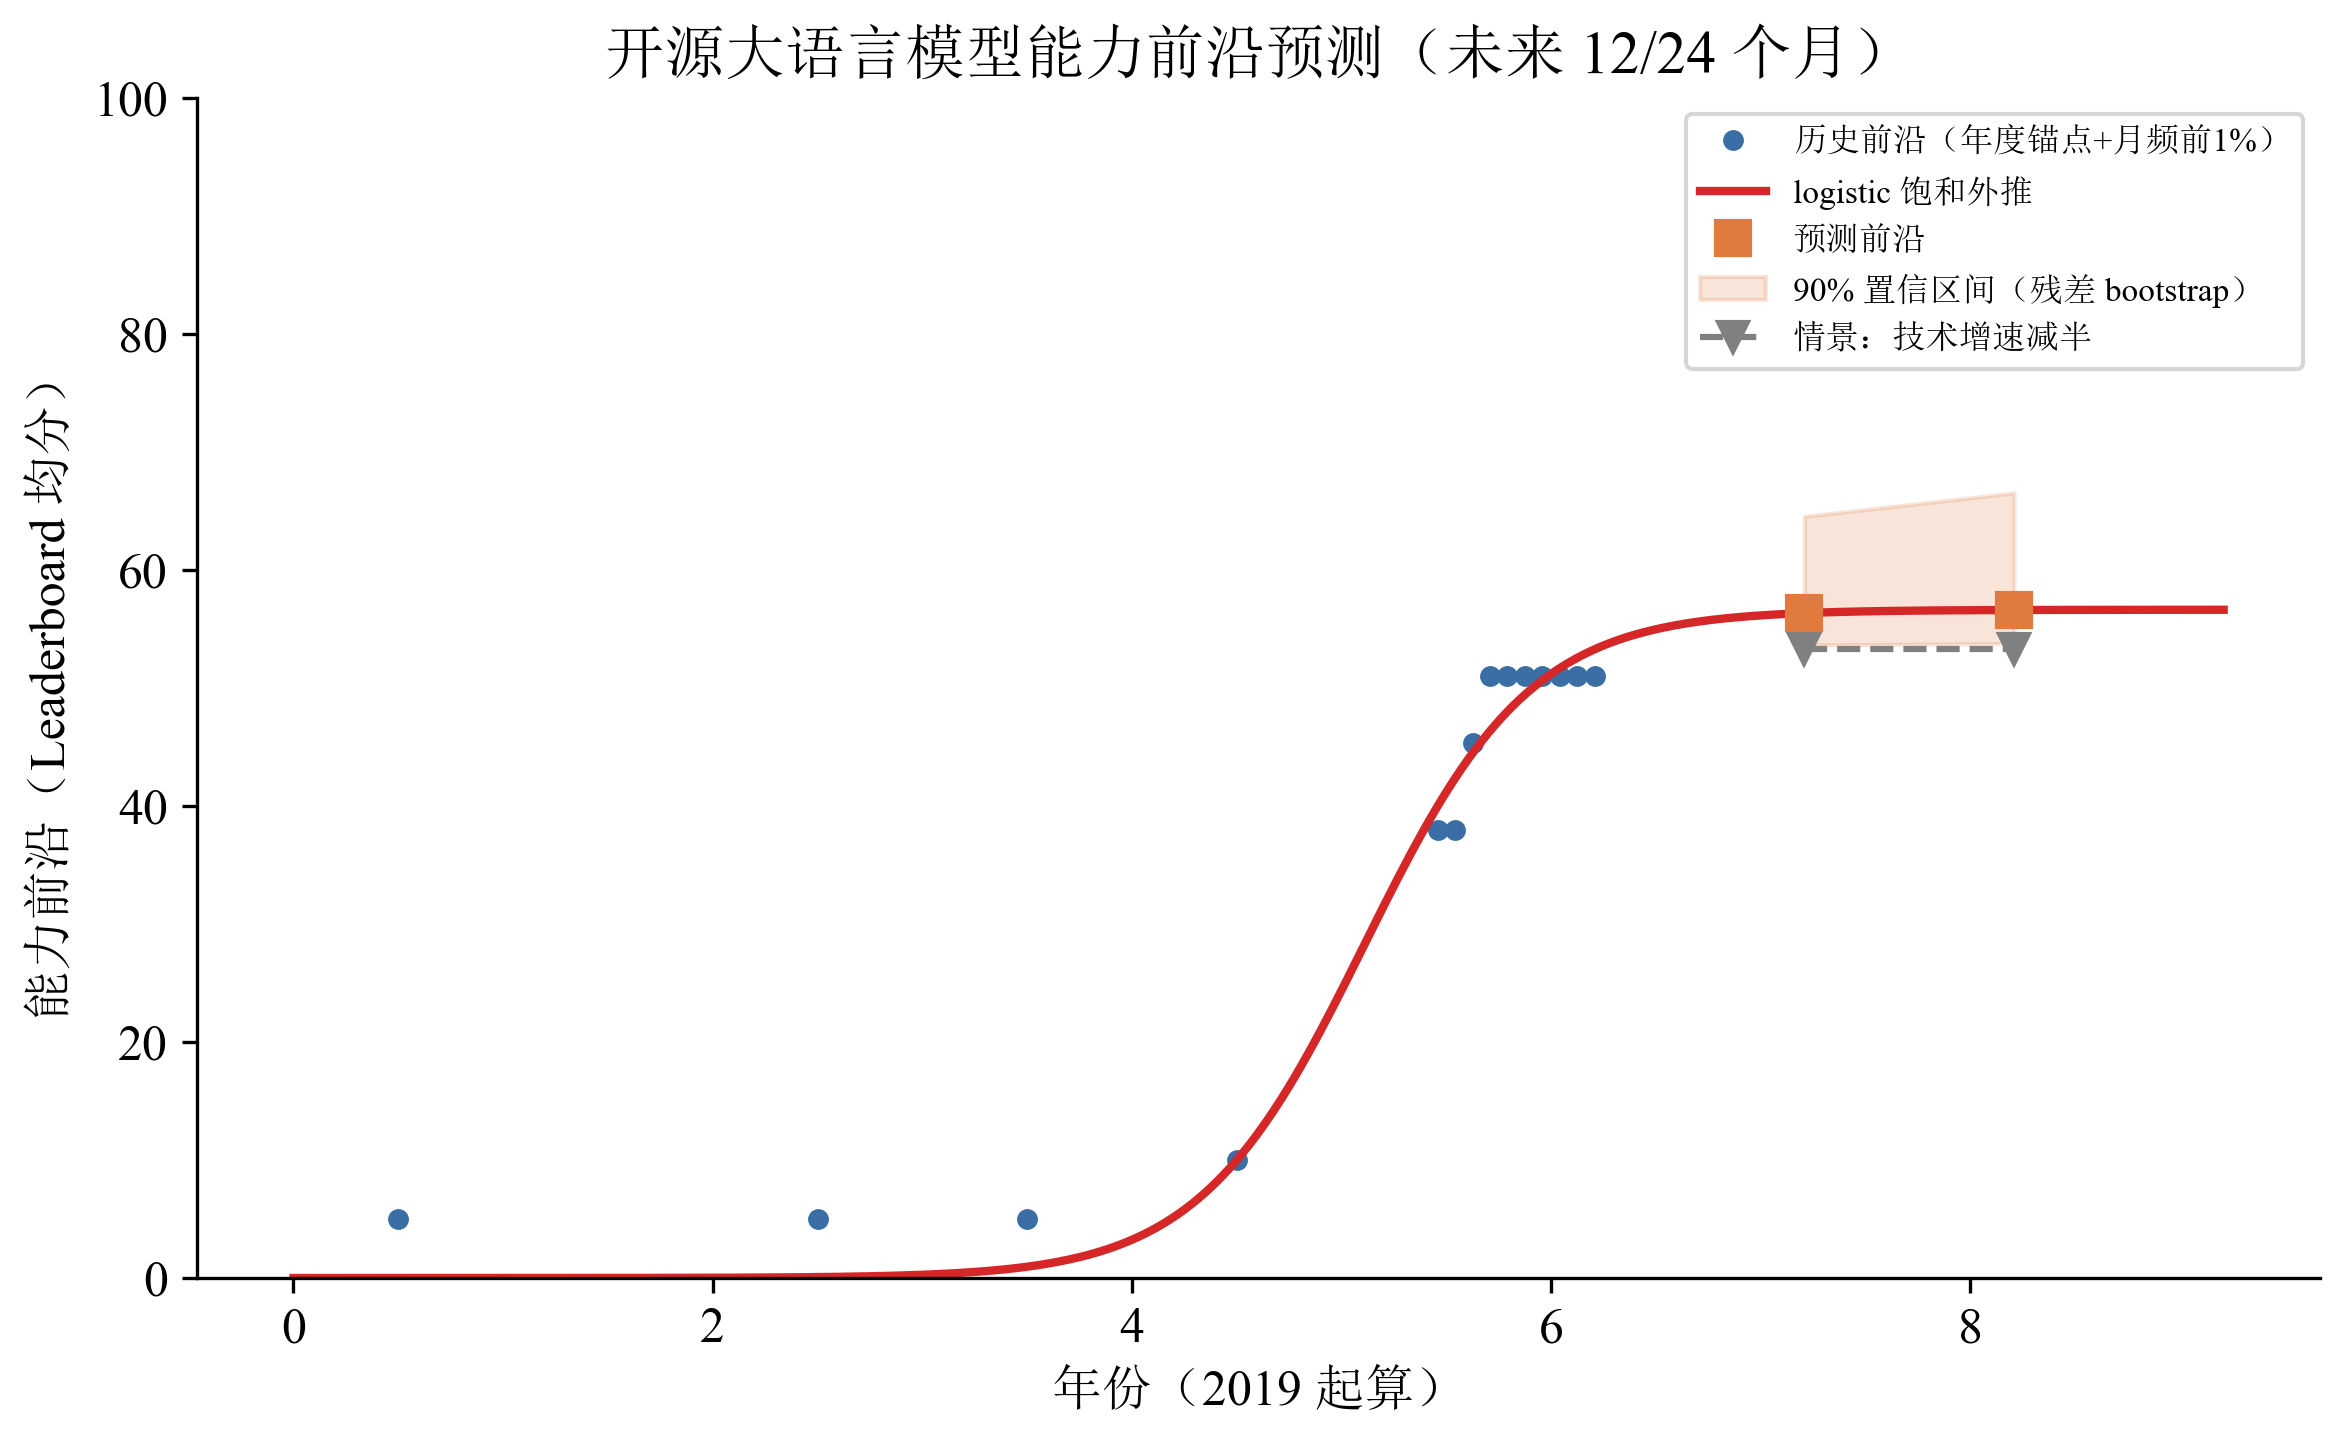
\includegraphics[width=0.72\textwidth]{求解/问题四/图片/图3_能力前沿预测.png}
  \caption{开源大语言模型能力前沿预测（未来 12/24 个月）}
  \label{fig:p4_frontier}
\end{figure}

\begin{longtable}{>{\centering\arraybackslash}p{0.16\textwidth}>{\centering\arraybackslash}p{0.12\textwidth}>{\centering\arraybackslash}p{0.11\textwidth}>{\centering\arraybackslash}p{0.11\textwidth}>{\centering\arraybackslash}p{0.12\textwidth}>{\raggedright\arraybackslash}p{0.22\textwidth}}
  \caption{能力前沿预测及不确定性（满分 100）}
  \label{tab:p4_frontier} \\
  \toprule
  前瞻期 & logistic 预测 & 下界（5\%） & 上界（95\%） & 增速减半 & 结构外推（基准/放缓/扩容） \\
  \midrule
  \endfirsthead
  \caption{能力前沿预测及不确定性（续）} \\
  \toprule
  前瞻期 & logistic 预测 & 下界（5\%） & 上界（95\%） & 增速减半 & 结构外推（基准/放缓/扩容） \\
  \midrule
  \endhead
  \bottomrule
  \endfoot
  $+12$ 个月（2026-03） & 56.33 & 53.62 & 64.52 & 53.27 & 55.84 / 53.42 / 59.99 \\
  $+24$ 个月（2027-03） & 56.59 & 53.75 & 66.52 & 53.27 & 60.69 / 55.84 / 68.99 \\
\end{longtable}

logistic 拟合参数为 $K=56.61$、$r=2.523$、$t_0=5.11$（自 2019 年起算），拟合 $R^2=0.975$。由表\ref{tab:p4_frontier}可知：（1）曲线外推给出未来 12/24 个月前沿约 $56.3$ 与 $56.6$，$90\%$ 置信区间分别为 $[53.6,64.5]$ 与 $[53.8,66.5]$；（2）若算力增长放缓、非规模技术增速减半，前沿将降至 $53.3$ 附近并在两年内基本停滞；（3）结构外推在三种情景下给出 $53.4\sim69.0$ 的区间。两条路线的差异来自“当前前沿是否已接近饱和”这一判断，因此本文以\textbf{区间}而非点值作为结论：未来 12 个月开源模型六维平均分前沿预计达 $53\sim60$，24 个月达 $54\sim69$；若算力增长显著放缓，前沿增速将接近停滞（约 $53\sim56$）。

需强调该预测的局限：本文可用的评测标准一致的窗口仅约 10 个月（2024-06 至 2025-03，Leaderboard v2 已停更），2019--2023 的锚点口径不完全一致（已剔除异常条目），故外推期约为一致窗口的 $1.2\sim2.4$ 倍，结论应理解为情景化区间而非精确点预测。

\textbf{4.逐任务聚合分析}

六维前沿与剩余空间如表\ref{tab:p4_task}与图\ref{fig:p4_task}所示，C8 子任务层面的结果见表\ref{tab:p4_sub}。

\begin{figure}[ht]
  \centering
  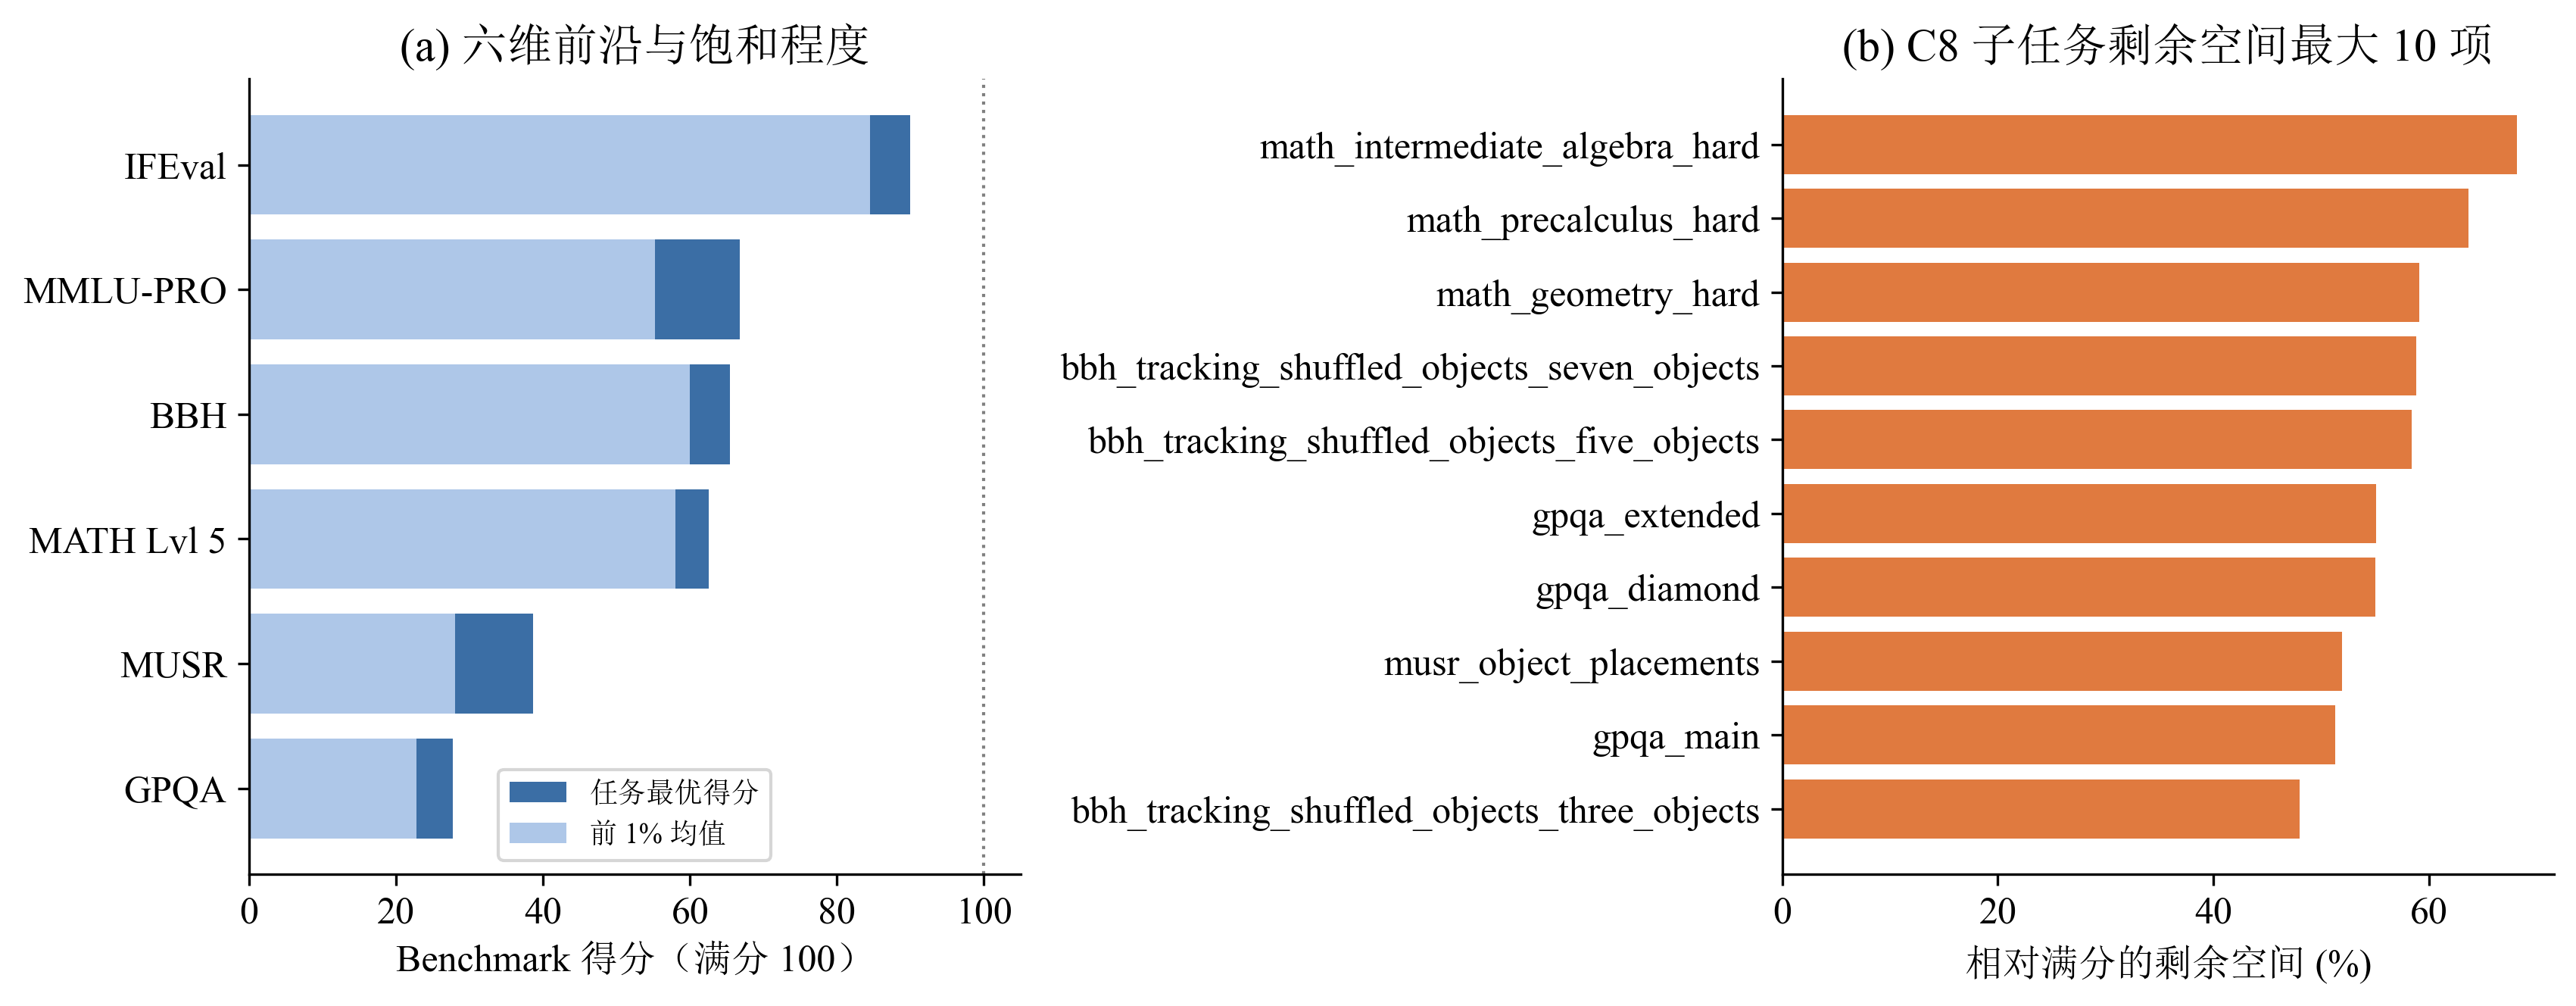
\includegraphics[width=0.92\textwidth]{求解/问题四/图片/图4_逐任务聚合.png}
  \caption{（左）六维 Benchmark 前沿与饱和程度；（右）C8 子任务剩余空间最大的 10 项}
  \label{fig:p4_task}
\end{figure}

\begin{longtable}{>{\centering\arraybackslash}p{0.18\textwidth}>{\centering\arraybackslash}p{0.13\textwidth}>{\centering\arraybackslash}p{0.15\textwidth}>{\centering\arraybackslash}p{0.15\textwidth}>{\raggedright\arraybackslash}p{0.21\textwidth}}
  \caption{六维 Benchmark 逐任务聚合结果（开源筛选集，$n=2{,}346$）}
  \label{tab:p4_task} \\
  \toprule
  任务 & 最优得分 & 前 1\% 均值 & 中位数 & 剩余空间 \\
  \midrule
  \endfirsthead
  \caption{六维 Benchmark 逐任务聚合结果（续）} \\
  \toprule
  任务 & 最优得分 & 前 1\% 均值 & 中位数 & 剩余空间 \\
  \midrule
  \endhead
  \bottomrule
  \endfoot
  IFEval & 89.98 & 84.45 & 43.51 & $10.0\%$ \\
  MMLU-PRO & 66.80 & 55.26 & 25.98 & $33.2\%$ \\
  BBH & 65.47 & 59.95 & 28.52 & $34.5\%$ \\
  MATH Lvl 5 & 62.54 & 58.02 & 9.93 & $37.5\%$ \\
  MUSR & 38.69 & 28.06 & 9.97 & $61.3\%$ \\
  GPQA & 27.74 & 22.80 & 5.70 & $72.3\%$ \\
\end{longtable}

\begin{longtable}{>{\raggedright\arraybackslash}p{0.42\textwidth}>{\centering\arraybackslash}p{0.12\textwidth}>{\centering\arraybackslash}p{0.12\textwidth}>{\centering\arraybackslash}p{0.12\textwidth}>{\raggedright\arraybackslash}p{0.12\textwidth}}
  \caption{C8 子任务层面剩余空间最大的 6 项（原始指标口径）}
  \label{tab:p4_sub} \\
  \toprule
  子任务 & 样本数 & 最优得分 & 前 5\% 均值 & 剩余空间 \\
  \midrule
  \endfirsthead
  \caption{C8 子任务剩余空间最大的 6 项（续）} \\
  \toprule
  子任务 & 样本数 & 最优得分 & 前 5\% 均值 & 剩余空间 \\
  \midrule
  \endhead
  \bottomrule
  \endfoot
  math\_intermediate\_algebra\_hard（MATH） & 962 & 31.79 & 20.11 & $68.2\%$ \\
  math\_precalculus\_hard（MATH） & 962 & 36.30 & 22.89 & $63.7\%$ \\
  math\_geometry\_hard（MATH） & 962 & 40.91 & 28.72 & $59.1\%$ \\
  bbh\_tracking\_shuffled\_objects\_seven（BBH） & 964 & 41.20 & 32.67 & $58.8\%$ \\
  bbh\_tracking\_shuffled\_objects\_five（BBH） & 964 & 41.60 & 31.24 & $58.4\%$ \\
  gpqa\_extended（GPQA） & 961 & 44.87 & 39.74 & $55.1\%$ \\
\end{longtable}

由表\ref{tab:p4_task}与表\ref{tab:p4_sub}可知：（1）六维能力发展极不均衡，指令遵循（IFEval，$89.98$）已接近满分、剩余空间仅 $10.0\%$，而研究生级问答（GPQA，$27.74$）与多轮推理（MUSR，$38.69$）远未饱和，剩余空间分别达 $72.3\%$ 与 $61.3\%$。（2）C8 子任务层面进一步定位了瓶颈：MATH-Hard 中的中级代数、预备微积分、几何三个子任务最优得分仅 $31.8\sim40.9$（该类别 7 个子任务的平均最优得分为 $55.5$，而整体中位数低至 $3.7$），BBH 中“跟踪被洗牌对象”类多步状态推理子任务最优得分约 $41$，GPQA 的 extended 子集为 $44.9$，这些是未来能力增量的主要方向。（3）C8 各类别的中位数普遍远低于最优值（BBH 中位数 $48.8$ 对最优 $81.8$；MATH 中位数 $3.7$ 对最优 $55.5$），说明开源社区的能力分布高度长尾，前列模型与总体水平差距巨大。

\textbf{5.附件 C4 的宏观证据与“算力增长放缓”情景校验}

C4 的宏观趋势如图\ref{fig:p4_c4}所示。

\begin{figure}[ht]
  \centering
  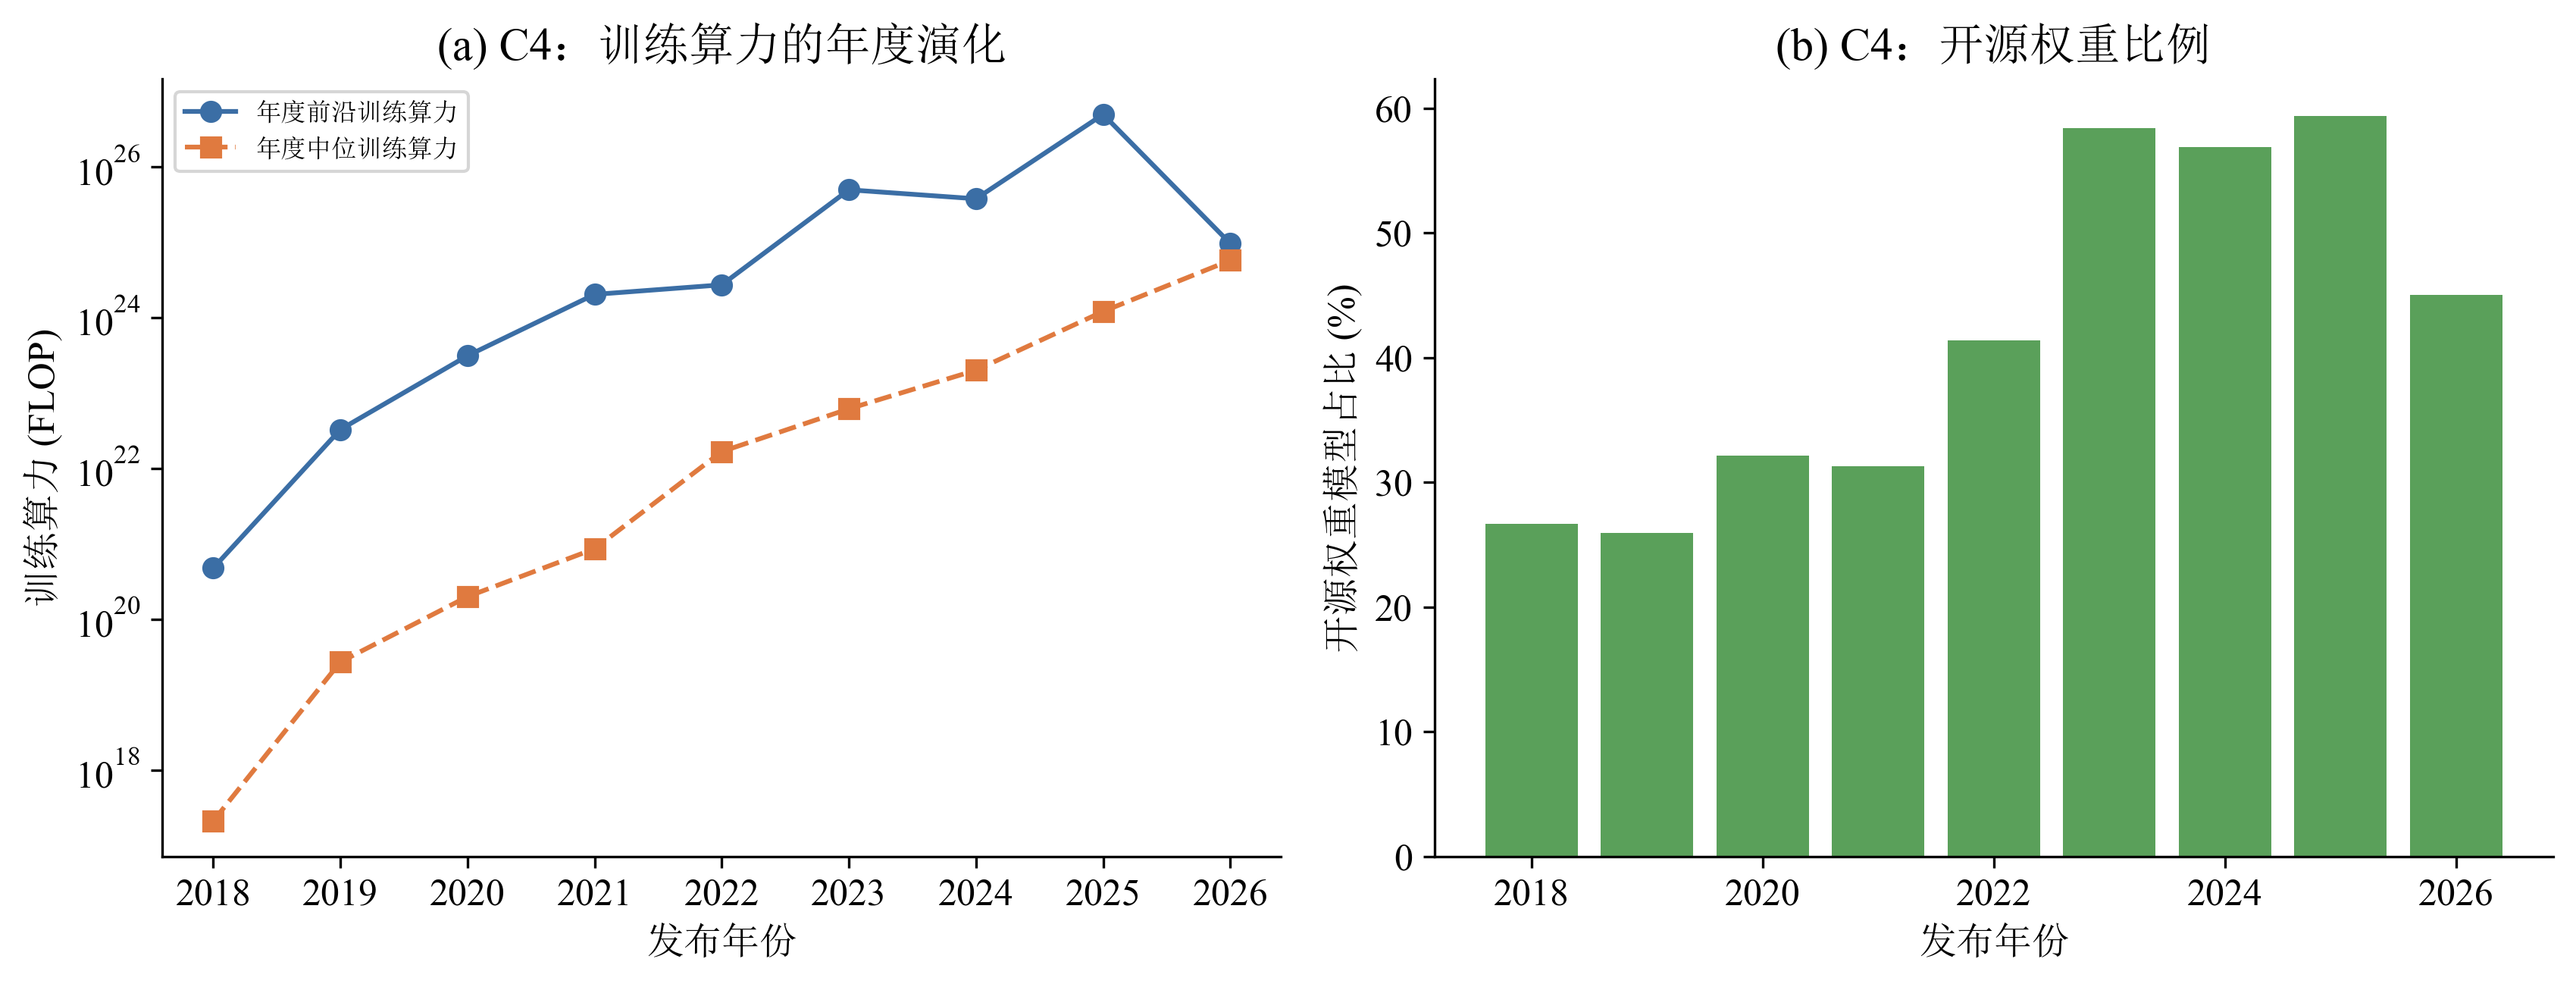
\includegraphics[width=0.92\textwidth]{求解/问题四/图片/图5_C4宏观趋势.png}
  \caption{C4 宏观证据（左：训练算力的年度演化；右：开源权重模型占比）}
  \label{fig:p4_c4}
\end{figure}

由图\ref{fig:p4_c4}可知：（1）C4 中 Language 域模型的前沿训练算力持续增长，对数尺度上的年增速约 $+0.589$ 个数量级（约 $3.88$ 倍/年），表明近年算力投入仍在快速扩张；但年际波动明显（2024 年前沿算力低于 2023 年，2025 年再创新高），说明算力增速并非单调外推、存在阶段性放缓的可能，这也正是本文把“算力增长放缓”作为**情景**（非规模增速减半）而非基准假设、并同时给出基准情景的原因。（2）开源权重模型的占比由 2018 年的 $26.7\%$ 持续上升至 2025 年的 $59.4\%$，说明本文以开源筛选样本刻画“能力前沿”具有良好的代表性与可持续性。（3）C4 中共有 1{,}390 条记录含训练算力、1{,}424 条含训练数据量、2{,}653 条标注开源权重（Yes 1{,}325、No 1{,}328）。需要说明的是，C4 的模型命名体系与 C1 不通用（规范化名称匹配仅命中 1 条），故 C4 仅作宏观尺度证据，不与 C1 逐行合并。

综合以上结果，本节完成了问题四的求解：明确并执行了时间轴、开源筛选与模型类型三类口径；完成了 C8 的逐任务聚合（1{,}860 个模型、37 个子任务维度）并与 C1 交叉校验；建立了分层 Loss—Benchmark 桥接并量化了映射误差；用面板回归分离出规模扩张与非规模技术进步的贡献（长周期各约 $50\%$，近端一致窗口内非规模因素占 $95.4\%$）；给出了未来 12/24 个月能力前沿的情景化预测区间与逐任务瓶颈定位。

